\chapter{Serie compleja de \emph{Fourier} y espectros discretos de frecuencia}

\section{Números complejos}
\begin{figure}[H]
    \centering
    % GNUPLOT: LaTeX picture with Postscript
\begingroup
  \makeatletter
  \providecommand\color[2][]{%
    \GenericError{(gnuplot) \space\space\space\@spaces}{%
      Package color not loaded in conjunction with
      terminal option `colourtext'%
    }{See the gnuplot documentation for explanation.%
    }{Either use 'blacktext' in gnuplot or load the package
      color.sty in LaTeX.}%
    \renewcommand\color[2][]{}%
  }%
  \providecommand\includegraphics[2][]{%
    \GenericError{(gnuplot) \space\space\space\@spaces}{%
      Package graphicx or graphics not loaded%
    }{See the gnuplot documentation for explanation.%
    }{The gnuplot epslatex terminal needs graphicx.sty or graphics.sty.}%
    \renewcommand\includegraphics[2][]{}%
  }%
  \providecommand\rotatebox[2]{#2}%
  \@ifundefined{ifGPcolor}{%
    \newif\ifGPcolor
    \GPcolorfalse
  }{}%
  \@ifundefined{ifGPblacktext}{%
    \newif\ifGPblacktext
    \GPblacktexttrue
  }{}%
  % define a \g@addto@macro without @ in the name:
  \let\gplgaddtomacro\g@addto@macro
  % define empty templates for all commands taking text:
  \gdef\gplbacktext{}%
  \gdef\gplfronttext{}%
  \makeatother
  \ifGPblacktext
    % no textcolor at all
    \def\colorrgb#1{}%
    \def\colorgray#1{}%
  \else
    % gray or color?
    \ifGPcolor
      \def\colorrgb#1{\color[rgb]{#1}}%
      \def\colorgray#1{\color[gray]{#1}}%
      \expandafter\def\csname LTw\endcsname{\color{white}}%
      \expandafter\def\csname LTb\endcsname{\color{black}}%
      \expandafter\def\csname LTa\endcsname{\color{black}}%
      \expandafter\def\csname LT0\endcsname{\color[rgb]{1,0,0}}%
      \expandafter\def\csname LT1\endcsname{\color[rgb]{0,1,0}}%
      \expandafter\def\csname LT2\endcsname{\color[rgb]{0,0,1}}%
      \expandafter\def\csname LT3\endcsname{\color[rgb]{1,0,1}}%
      \expandafter\def\csname LT4\endcsname{\color[rgb]{0,1,1}}%
      \expandafter\def\csname LT5\endcsname{\color[rgb]{1,1,0}}%
      \expandafter\def\csname LT6\endcsname{\color[rgb]{0,0,0}}%
      \expandafter\def\csname LT7\endcsname{\color[rgb]{1,0.3,0}}%
      \expandafter\def\csname LT8\endcsname{\color[rgb]{0.5,0.5,0.5}}%
    \else
      % gray
      \def\colorrgb#1{\color{black}}%
      \def\colorgray#1{\color[gray]{#1}}%
      \expandafter\def\csname LTw\endcsname{\color{white}}%
      \expandafter\def\csname LTb\endcsname{\color{black}}%
      \expandafter\def\csname LTa\endcsname{\color{black}}%
      \expandafter\def\csname LT0\endcsname{\color{black}}%
      \expandafter\def\csname LT1\endcsname{\color{black}}%
      \expandafter\def\csname LT2\endcsname{\color{black}}%
      \expandafter\def\csname LT3\endcsname{\color{black}}%
      \expandafter\def\csname LT4\endcsname{\color{black}}%
      \expandafter\def\csname LT5\endcsname{\color{black}}%
      \expandafter\def\csname LT6\endcsname{\color{black}}%
      \expandafter\def\csname LT7\endcsname{\color{black}}%
      \expandafter\def\csname LT8\endcsname{\color{black}}%
    \fi
  \fi
    \setlength{\unitlength}{0.0500bp}%
    \ifx\gptboxheight\undefined%
      \newlength{\gptboxheight}%
      \newlength{\gptboxwidth}%
      \newsavebox{\gptboxtext}%
    \fi%
    \setlength{\fboxrule}{0.5pt}%
    \setlength{\fboxsep}{1pt}%
    \definecolor{tbcol}{rgb}{1,1,1}%
\begin{picture}(2880.00,2880.00)%
    \gplgaddtomacro\gplbacktext{%
      \csname LTb\endcsname%%
      \put(614,192){\makebox(0,0)[r]{\strut{}}}%
      \put(614,697){\makebox(0,0)[r]{\strut{}}}%
      \put(614,1203){\makebox(0,0)[r]{\strut{}}}%
      \put(614,1708){\makebox(0,0)[r]{\strut{}}}%
      \put(614,2214){\makebox(0,0)[r]{\strut{}}}%
      \put(614,2719){\makebox(0,0)[r]{\strut{}}}%
      \put(240,474){\makebox(0,0){\strut{}}}%
      \put(710,474){\makebox(0,0){\strut{}}}%
      \put(1180,474){\makebox(0,0){\strut{}}}%
      \put(1651,474){\makebox(0,0){\strut{}}}%
      \put(2121,474){\makebox(0,0){\strut{}}}%
      \put(2591,474){\makebox(0,0){\strut{}}}%
      \csname LTb\endcsname%%
      \put(3061,697){\makebox(0,0)[l]{\strut{}$\mathbb{R}e$}}%
      \put(875,2845){\makebox(0,0)[l]{\strut{}$\mathbb{I}m$}}%
      \put(1886,2441){\makebox(0,0)[l]{\strut{}$z=a+jb$}}%
      \put(2074,521){\makebox(0,0)[l]{\strut{}$a$}}%
      \put(358,2239){\makebox(0,0)[l]{\strut{}$jb$}}%
      \put(1274,900){\makebox(0,0)[l]{\strut{}$\theta$}}%
    }%
    \gplgaddtomacro\gplfronttext{%
    }%
    \gplgaddtomacro\gplbacktext{%
      \csname LTb\endcsname%%
      \put(614,192){\makebox(0,0)[r]{\strut{}}}%
      \put(614,697){\makebox(0,0)[r]{\strut{}}}%
      \put(614,1203){\makebox(0,0)[r]{\strut{}}}%
      \put(614,1708){\makebox(0,0)[r]{\strut{}}}%
      \put(614,2214){\makebox(0,0)[r]{\strut{}}}%
      \put(614,2719){\makebox(0,0)[r]{\strut{}}}%
      \put(240,474){\makebox(0,0){\strut{}}}%
      \put(710,474){\makebox(0,0){\strut{}}}%
      \put(1180,474){\makebox(0,0){\strut{}}}%
      \put(1651,474){\makebox(0,0){\strut{}}}%
      \put(2121,474){\makebox(0,0){\strut{}}}%
      \put(2591,474){\makebox(0,0){\strut{}}}%
      \csname LTb\endcsname%%
      \put(3061,697){\makebox(0,0)[l]{\strut{}$\mathbb{R}e$}}%
      \put(875,2845){\makebox(0,0)[l]{\strut{}$\mathbb{I}m$}}%
      \put(1886,2441){\makebox(0,0)[l]{\strut{}$z=a+jb$}}%
      \put(2074,521){\makebox(0,0)[l]{\strut{}$a$}}%
      \put(358,2239){\makebox(0,0)[l]{\strut{}$jb$}}%
      \put(1274,900){\makebox(0,0)[l]{\strut{}$\theta$}}%
    }%
    \gplgaddtomacro\gplfronttext{%
    }%
    \gplbacktext
    \put(0,0){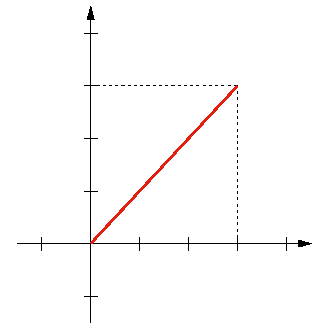
\includegraphics[width={144.00bp},height={144.00bp}]{figura_03_01}}%
    \gplfronttext
  \end{picture}%
\endgroup

\end{figure}
\begin{center}
    Unidad imaginaria: $i=j=\sqrt{-1}$\\
    Forma rectangular: $z=a+jb$\\
    Módulo: $|z|=\sqrt{a^2+b^2}$\\
    Argumento: $\theta=\arctan(\frac{b}{a})$\\
\end{center}

Forma polar:
\begin{equation*}
    z=|z|\cos(\theta)+j|z|\sen(\theta)
        =|z|(\cos(\theta)+j\sen(\theta))
\end{equation*}

Formula de \emph{Euler}:
\begin{equation}
    e^{j\theta}=\cos(\theta)+j\sen(\theta)
\end{equation}

Por tanto:
\begin{equation*}
    z=|z|e^{j\theta}
\end{equation*}

Forma exponencial o fasorial:
\begin{equation*}
    z=|z|\angle\theta
\end{equation*}

\subsection{Formas complejas del seno y coseno}
\begin{equation}
    e^{j\theta}=\cos(\theta)+j\sen(\theta)
    \label{e1}
\end{equation}
\begin{equation}
    e^{-j\theta}=\cos(\theta)-j\sen(\theta)
    \label{e2}
\end{equation}

Sumando las ecuaciones~\ref{e1} y~\ref{e2}:
\begin{equation*}
    e^{j\theta}+e^{-j\theta}=2\cos(\theta)
\end{equation*}
\begin{equation}
    \cos(\theta)=\frac{e^{j\theta}+e^{-j\theta}}{2}
\end{equation}

Restando las ecuaciones~\ref{e1} y~\ref{e2}:
\begin{equation*}
    e^{j\theta}-e^{-j\theta}=2j\sen(\theta)
\end{equation*}
\begin{equation}
    \sen(\theta)=\frac{e^{j\theta}-e^{-j\theta}}{2j}
\end{equation}

\subsection{Conjugado}
\begin{figure}[H]
    \centering
    % GNUPLOT: LaTeX picture with Postscript
\begingroup
  \makeatletter
  \providecommand\color[2][]{%
    \GenericError{(gnuplot) \space\space\space\@spaces}{%
      Package color not loaded in conjunction with
      terminal option `colourtext'%
    }{See the gnuplot documentation for explanation.%
    }{Either use 'blacktext' in gnuplot or load the package
      color.sty in LaTeX.}%
    \renewcommand\color[2][]{}%
  }%
  \providecommand\includegraphics[2][]{%
    \GenericError{(gnuplot) \space\space\space\@spaces}{%
      Package graphicx or graphics not loaded%
    }{See the gnuplot documentation for explanation.%
    }{The gnuplot epslatex terminal needs graphicx.sty or graphics.sty.}%
    \renewcommand\includegraphics[2][]{}%
  }%
  \providecommand\rotatebox[2]{#2}%
  \@ifundefined{ifGPcolor}{%
    \newif\ifGPcolor
    \GPcolorfalse
  }{}%
  \@ifundefined{ifGPblacktext}{%
    \newif\ifGPblacktext
    \GPblacktexttrue
  }{}%
  % define a \g@addto@macro without @ in the name:
  \let\gplgaddtomacro\g@addto@macro
  % define empty templates for all commands taking text:
  \gdef\gplbacktext{}%
  \gdef\gplfronttext{}%
  \makeatother
  \ifGPblacktext
    % no textcolor at all
    \def\colorrgb#1{}%
    \def\colorgray#1{}%
  \else
    % gray or color?
    \ifGPcolor
      \def\colorrgb#1{\color[rgb]{#1}}%
      \def\colorgray#1{\color[gray]{#1}}%
      \expandafter\def\csname LTw\endcsname{\color{white}}%
      \expandafter\def\csname LTb\endcsname{\color{black}}%
      \expandafter\def\csname LTa\endcsname{\color{black}}%
      \expandafter\def\csname LT0\endcsname{\color[rgb]{1,0,0}}%
      \expandafter\def\csname LT1\endcsname{\color[rgb]{0,1,0}}%
      \expandafter\def\csname LT2\endcsname{\color[rgb]{0,0,1}}%
      \expandafter\def\csname LT3\endcsname{\color[rgb]{1,0,1}}%
      \expandafter\def\csname LT4\endcsname{\color[rgb]{0,1,1}}%
      \expandafter\def\csname LT5\endcsname{\color[rgb]{1,1,0}}%
      \expandafter\def\csname LT6\endcsname{\color[rgb]{0,0,0}}%
      \expandafter\def\csname LT7\endcsname{\color[rgb]{1,0.3,0}}%
      \expandafter\def\csname LT8\endcsname{\color[rgb]{0.5,0.5,0.5}}%
    \else
      % gray
      \def\colorrgb#1{\color{black}}%
      \def\colorgray#1{\color[gray]{#1}}%
      \expandafter\def\csname LTw\endcsname{\color{white}}%
      \expandafter\def\csname LTb\endcsname{\color{black}}%
      \expandafter\def\csname LTa\endcsname{\color{black}}%
      \expandafter\def\csname LT0\endcsname{\color{black}}%
      \expandafter\def\csname LT1\endcsname{\color{black}}%
      \expandafter\def\csname LT2\endcsname{\color{black}}%
      \expandafter\def\csname LT3\endcsname{\color{black}}%
      \expandafter\def\csname LT4\endcsname{\color{black}}%
      \expandafter\def\csname LT5\endcsname{\color{black}}%
      \expandafter\def\csname LT6\endcsname{\color{black}}%
      \expandafter\def\csname LT7\endcsname{\color{black}}%
      \expandafter\def\csname LT8\endcsname{\color{black}}%
    \fi
  \fi
    \setlength{\unitlength}{0.0500bp}%
    \ifx\gptboxheight\undefined%
      \newlength{\gptboxheight}%
      \newlength{\gptboxwidth}%
      \newsavebox{\gptboxtext}%
    \fi%
    \setlength{\fboxrule}{0.5pt}%
    \setlength{\fboxsep}{1pt}%
    \definecolor{tbcol}{rgb}{1,1,1}%
\begin{picture}(3600.00,3600.00)%
    \gplgaddtomacro\gplbacktext{%
      \csname LTb\endcsname%%
      \put(1680,192){\makebox(0,0)[r]{\strut{}}}%
      \put(1680,598){\makebox(0,0)[r]{\strut{}}}%
      \put(1680,1004){\makebox(0,0)[r]{\strut{}}}%
      \put(1680,1410){\makebox(0,0)[r]{\strut{}}}%
      \put(1680,1816){\makebox(0,0)[r]{\strut{}}}%
      \put(1680,2221){\makebox(0,0)[r]{\strut{}}}%
      \put(1680,2627){\makebox(0,0)[r]{\strut{}}}%
      \put(1680,3033){\makebox(0,0)[r]{\strut{}}}%
      \put(1680,3439){\makebox(0,0)[r]{\strut{}}}%
      \put(240,1593){\makebox(0,0){\strut{}}}%
      \put(624,1593){\makebox(0,0){\strut{}}}%
      \put(1008,1593){\makebox(0,0){\strut{}}}%
      \put(1392,1593){\makebox(0,0){\strut{}}}%
      \put(1776,1593){\makebox(0,0){\strut{}}}%
      \put(2159,1593){\makebox(0,0){\strut{}}}%
      \put(2543,1593){\makebox(0,0){\strut{}}}%
      \put(2927,1593){\makebox(0,0){\strut{}}}%
      \put(3311,1593){\makebox(0,0){\strut{}}}%
      \csname LTb\endcsname%%
      \put(3695,1816){\makebox(0,0)[l]{\strut{}$\mathbb{R}e$}}%
      \put(1910,3540){\makebox(0,0)[l]{\strut{}$\mathbb{I}m$}}%
      \put(2927,3216){\makebox(0,0)[l]{\strut{}$z$}}%
      \put(2927,415){\makebox(0,0)[l]{\strut{}$z*$}}%
      \put(2889,1673){\makebox(0,0)[l]{\strut{}$a$}}%
      \put(1488,3053){\makebox(0,0)[l]{\strut{}$jb$}}%
      \put(1392,578){\makebox(0,0)[l]{\strut{}$-jb$}}%
      \put(2236,1978){\makebox(0,0)[l]{\strut{}$\theta$}}%
      \put(2236,1572){\makebox(0,0)[l]{\strut{}$-\theta$}}%
    }%
    \gplgaddtomacro\gplfronttext{%
    }%
    \gplgaddtomacro\gplbacktext{%
      \csname LTb\endcsname%%
      \put(1680,192){\makebox(0,0)[r]{\strut{}}}%
      \put(1680,598){\makebox(0,0)[r]{\strut{}}}%
      \put(1680,1004){\makebox(0,0)[r]{\strut{}}}%
      \put(1680,1410){\makebox(0,0)[r]{\strut{}}}%
      \put(1680,1816){\makebox(0,0)[r]{\strut{}}}%
      \put(1680,2221){\makebox(0,0)[r]{\strut{}}}%
      \put(1680,2627){\makebox(0,0)[r]{\strut{}}}%
      \put(1680,3033){\makebox(0,0)[r]{\strut{}}}%
      \put(1680,3439){\makebox(0,0)[r]{\strut{}}}%
      \put(240,1593){\makebox(0,0){\strut{}}}%
      \put(624,1593){\makebox(0,0){\strut{}}}%
      \put(1008,1593){\makebox(0,0){\strut{}}}%
      \put(1392,1593){\makebox(0,0){\strut{}}}%
      \put(1776,1593){\makebox(0,0){\strut{}}}%
      \put(2159,1593){\makebox(0,0){\strut{}}}%
      \put(2543,1593){\makebox(0,0){\strut{}}}%
      \put(2927,1593){\makebox(0,0){\strut{}}}%
      \put(3311,1593){\makebox(0,0){\strut{}}}%
      \csname LTb\endcsname%%
      \put(3695,1816){\makebox(0,0)[l]{\strut{}$\mathbb{R}e$}}%
      \put(1910,3540){\makebox(0,0)[l]{\strut{}$\mathbb{I}m$}}%
      \put(2927,3216){\makebox(0,0)[l]{\strut{}$z$}}%
      \put(2927,415){\makebox(0,0)[l]{\strut{}$z*$}}%
      \put(2889,1673){\makebox(0,0)[l]{\strut{}$a$}}%
      \put(1488,3053){\makebox(0,0)[l]{\strut{}$jb$}}%
      \put(1392,578){\makebox(0,0)[l]{\strut{}$-jb$}}%
      \put(2236,1978){\makebox(0,0)[l]{\strut{}$\theta$}}%
      \put(2236,1572){\makebox(0,0)[l]{\strut{}$-\theta$}}%
    }%
    \gplgaddtomacro\gplfronttext{%
    }%
    \gplgaddtomacro\gplbacktext{%
      \csname LTb\endcsname%%
      \put(1680,192){\makebox(0,0)[r]{\strut{}}}%
      \put(1680,598){\makebox(0,0)[r]{\strut{}}}%
      \put(1680,1004){\makebox(0,0)[r]{\strut{}}}%
      \put(1680,1410){\makebox(0,0)[r]{\strut{}}}%
      \put(1680,1816){\makebox(0,0)[r]{\strut{}}}%
      \put(1680,2221){\makebox(0,0)[r]{\strut{}}}%
      \put(1680,2627){\makebox(0,0)[r]{\strut{}}}%
      \put(1680,3033){\makebox(0,0)[r]{\strut{}}}%
      \put(1680,3439){\makebox(0,0)[r]{\strut{}}}%
      \put(240,1593){\makebox(0,0){\strut{}}}%
      \put(624,1593){\makebox(0,0){\strut{}}}%
      \put(1008,1593){\makebox(0,0){\strut{}}}%
      \put(1392,1593){\makebox(0,0){\strut{}}}%
      \put(1776,1593){\makebox(0,0){\strut{}}}%
      \put(2159,1593){\makebox(0,0){\strut{}}}%
      \put(2543,1593){\makebox(0,0){\strut{}}}%
      \put(2927,1593){\makebox(0,0){\strut{}}}%
      \put(3311,1593){\makebox(0,0){\strut{}}}%
      \csname LTb\endcsname%%
      \put(3695,1816){\makebox(0,0)[l]{\strut{}$\mathbb{R}e$}}%
      \put(1910,3540){\makebox(0,0)[l]{\strut{}$\mathbb{I}m$}}%
      \put(2927,3216){\makebox(0,0)[l]{\strut{}$z$}}%
      \put(2927,415){\makebox(0,0)[l]{\strut{}$z*$}}%
      \put(2889,1673){\makebox(0,0)[l]{\strut{}$a$}}%
      \put(1488,3053){\makebox(0,0)[l]{\strut{}$jb$}}%
      \put(1392,578){\makebox(0,0)[l]{\strut{}$-jb$}}%
      \put(2236,1978){\makebox(0,0)[l]{\strut{}$\theta$}}%
      \put(2236,1572){\makebox(0,0)[l]{\strut{}$-\theta$}}%
    }%
    \gplgaddtomacro\gplfronttext{%
    }%
    \gplgaddtomacro\gplbacktext{%
      \csname LTb\endcsname%%
      \put(1680,192){\makebox(0,0)[r]{\strut{}}}%
      \put(1680,598){\makebox(0,0)[r]{\strut{}}}%
      \put(1680,1004){\makebox(0,0)[r]{\strut{}}}%
      \put(1680,1410){\makebox(0,0)[r]{\strut{}}}%
      \put(1680,1816){\makebox(0,0)[r]{\strut{}}}%
      \put(1680,2221){\makebox(0,0)[r]{\strut{}}}%
      \put(1680,2627){\makebox(0,0)[r]{\strut{}}}%
      \put(1680,3033){\makebox(0,0)[r]{\strut{}}}%
      \put(1680,3439){\makebox(0,0)[r]{\strut{}}}%
      \put(240,1593){\makebox(0,0){\strut{}}}%
      \put(624,1593){\makebox(0,0){\strut{}}}%
      \put(1008,1593){\makebox(0,0){\strut{}}}%
      \put(1392,1593){\makebox(0,0){\strut{}}}%
      \put(1776,1593){\makebox(0,0){\strut{}}}%
      \put(2159,1593){\makebox(0,0){\strut{}}}%
      \put(2543,1593){\makebox(0,0){\strut{}}}%
      \put(2927,1593){\makebox(0,0){\strut{}}}%
      \put(3311,1593){\makebox(0,0){\strut{}}}%
      \csname LTb\endcsname%%
      \put(3695,1816){\makebox(0,0)[l]{\strut{}$\mathbb{R}e$}}%
      \put(1910,3540){\makebox(0,0)[l]{\strut{}$\mathbb{I}m$}}%
      \put(2927,3216){\makebox(0,0)[l]{\strut{}$z$}}%
      \put(2927,415){\makebox(0,0)[l]{\strut{}$z*$}}%
      \put(2889,1673){\makebox(0,0)[l]{\strut{}$a$}}%
      \put(1488,3053){\makebox(0,0)[l]{\strut{}$jb$}}%
      \put(1392,578){\makebox(0,0)[l]{\strut{}$-jb$}}%
      \put(2236,1978){\makebox(0,0)[l]{\strut{}$\theta$}}%
      \put(2236,1572){\makebox(0,0)[l]{\strut{}$-\theta$}}%
    }%
    \gplgaddtomacro\gplfronttext{%
    }%
    \gplbacktext
    \put(0,0){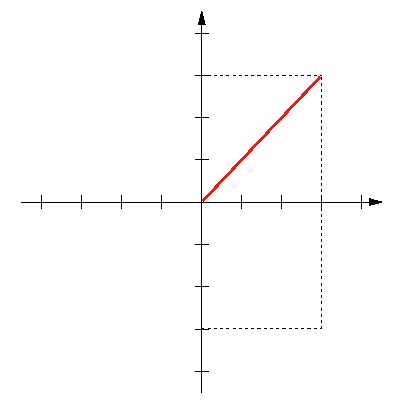
\includegraphics[width={180.00bp},height={180.00bp}]{figura_03_02}}%
    \gplfronttext
  \end{picture}%
\endgroup

\end{figure}
\begin{equation*}
    z=a+jb=|z|\angle\theta
\end{equation*}
\begin{equation*}
    z*=a-jb=|z|\angle-\theta
\end{equation*}
\begin{equation*}
    (z)(z*)={|z|}^2
\end{equation*}

\section{Serie compleja de \emph{Fourier}}
Partiendo de la serie trigonométrica de \emph{Fourier}:
\begin{equation*}
    f(t)=\frac{a_0}{2}+
    \sum_{n=1}^{\infty}\left[
        a_n\cos(n\omega_0\,t)+
        b_n\sen(n\omega_0\,t)
    \right]
\end{equation*}
\begin{equation*}
    f(t)=\frac{a_0}{2}+
    \sum_{n=1}^{\infty}\left[
        a_n\left(
            \frac{e^{jn\omega_0\,t}+e^{-jn\omega_0\,t}
            }{2}
        \right)+
        b_n\left(
            \frac{e^{jn\omega_0\,t}+e^{-jn\omega_0\,t}
            }{2j}
        \right)
    \right]
\end{equation*}
\begin{equation*}
    \frac{1}{j}=-j
\end{equation*}
\begin{equation*}
    f(t)=\frac{a_0}{2}+
    \sum_{n=1}^{\infty}\left[
        a_n\left(
            \frac{e^{jn\omega_0\,t}+e^{-jn\omega_0\,t}
            }{2}
        \right)-
        jb_n\left(
            \frac{e^{jn\omega_0\,t}+e^{-jn\omega_0\,t}
            }{2}
        \right)
    \right]
\end{equation*}
\begin{equation*}
    f(t)=\frac{a_0}{2}+
    \sum_{n=1}^{\infty}\left[
        \left(\frac{a_n-jb_n}{2}\right)e^{jn\omega_0\,t}+
        \left(\frac{a_n+jb_n}{2}\right)e^{-jn\omega_0\,t}
    \right]
\end{equation*}
\begin{equation*}
    f(t)=\frac{a_0}{2}+
    \sum_{n=1}^{\infty}\left[
        \left(\frac{a_n-jb_n}{2}\right)e^{jn\omega_0\,t}
    \right]+
    \sum_{n=1}^{\infty}\left[
        \left(\frac{a_n+jb_n}{2}\right)e^{-jn\omega_0\,t}
    \right]
\end{equation*}
\begin{equation*}
    f(t)=\frac{a_0}{2}+
    \sum_{n=1}^{\infty}\left[
        \left(\frac{a_n-jb_n}{2}\right)e^{jn\omega_0\,t}
    \right]+
    \sum_{-n=1}^{\infty}\left[
        \left(\frac{a_{-n}+jb_{-n}}{2}\right)e^{jn\omega_0\,t}
    \right]
\end{equation*}
\begin{equation*}
    f(t)=\frac{a_0}{2}+
    \sum_{n=1}^{\infty}\left[
        \left(\frac{a_n-jb_n}{2}\right)e^{jn\omega_0\,t}
    \right]+
    \sum_{n=-1}^{-\infty}\left[
        \left(\frac{a_n+jb_n}{2}\right)e^{jn\omega_0\,t}
    \right]
\end{equation*}
\begin{equation*}
    f(t)=\frac{a_0}{2}+
    \sum_{\substack{n=-\infty\\n\neq0}}^{\infty}
        \left(\frac{a_n-jb_n}{2}\right)e^{jn\omega_0\,t}
\end{equation*}

Sean los coeficientes complejos de \emph{Fourier}:
\begin{equation*}
    c_n=\frac{a_n-jb_n}{2}
\end{equation*}
\begin{equation*}
    c_0=\frac{a_0}{2}
\end{equation*}

Entonces:
\begin{equation*}
    f(t)=c_0+\sum_{\substack{n=-\infty\\n\neq0}}^{\infty}c_n\,e^{jn\omega_0\,t}
\end{equation*}
\begin{equation}
    f(t)=\sum_{n=-\infty}^{\infty}c_n\,e^{jn\omega_0\,t}
\end{equation}

\subsection{Evaluación del coeficiente complejo de \emph{Fourier}}
\begin{equation*}
\begin{split}
    c_n
        &=\frac{a_n-jb_n}{2}\\
        &=\frac{1}{2}\left[
            \frac{2}{T}\int_0^T\,f(t)\cos(n\omega_0\,t)\,dt
            -j\frac{2}{T}\int_0^T\,f(t)\sen(n\omega_0\,t)\,dt
        \right]\\
        &=\frac{1}{T}\int_0^T\,f(t)\left[
            \cos(n\omega_0\,t)-j\sen(n\omega_0\,t)
        \right]dt\\
        &=\frac{1}{T}\int_0^T\,f(t)\,e^{-jn\omega_0\,t}\,dt\\
\end{split}
\end{equation*}
\begin{equation}
    c_n=\frac{1}{T}\int_0^T\,f(t)\,e^{-jn\omega_0\,t}\,dt
\end{equation}

En particular:
\begin{equation}
    c_0=\frac{1}{T}\int_0^T\,f(t)\,dt
\end{equation}

\subsection{Relación entre el coeficiente complejo y los coeficientes
trigonométricos}
\begin{equation*}
    c_n=\frac{a_n-jbn}{2}
        =\frac{a_n}{2}+j\frac{-b_n}{2}
\end{equation*}
\begin{equation*}
    \frac{a_n}{2}=\mathbb{R}e\{c_n\}
\end{equation*}
\begin{equation}
    a_n=2\,\mathbb{R}e\{c_n\}
\end{equation}
\begin{equation*}
    -\frac{b_n}{2}=\mathbb{I}m\{c_n\}
\end{equation*}
\begin{equation}
    b_n=-2\,\mathbb{I}m\{c_n\}
\end{equation}

\section{Ondas senoidales rectificadas}
\subsection{Rectificación de media onda}
\begin{equation*}
    f(t)=\begin{cases}
        A\sen(\omega_0\,t)&0<t<T/2\\
        0&T/2<t<T\\
    \end{cases}
\end{equation*}
\begin{equation*}
    T=\frac{2\pi}{\omega_0}
\end{equation*}
\begin{figure}[H]
    \centering
    % GNUPLOT: LaTeX picture with Postscript
\begingroup
  \makeatletter
  \providecommand\color[2][]{%
    \GenericError{(gnuplot) \space\space\space\@spaces}{%
      Package color not loaded in conjunction with
      terminal option `colourtext'%
    }{See the gnuplot documentation for explanation.%
    }{Either use 'blacktext' in gnuplot or load the package
      color.sty in LaTeX.}%
    \renewcommand\color[2][]{}%
  }%
  \providecommand\includegraphics[2][]{%
    \GenericError{(gnuplot) \space\space\space\@spaces}{%
      Package graphicx or graphics not loaded%
    }{See the gnuplot documentation for explanation.%
    }{The gnuplot epslatex terminal needs graphicx.sty or graphics.sty.}%
    \renewcommand\includegraphics[2][]{}%
  }%
  \providecommand\rotatebox[2]{#2}%
  \@ifundefined{ifGPcolor}{%
    \newif\ifGPcolor
    \GPcolorfalse
  }{}%
  \@ifundefined{ifGPblacktext}{%
    \newif\ifGPblacktext
    \GPblacktexttrue
  }{}%
  % define a \g@addto@macro without @ in the name:
  \let\gplgaddtomacro\g@addto@macro
  % define empty templates for all commands taking text:
  \gdef\gplbacktext{}%
  \gdef\gplfronttext{}%
  \makeatother
  \ifGPblacktext
    % no textcolor at all
    \def\colorrgb#1{}%
    \def\colorgray#1{}%
  \else
    % gray or color?
    \ifGPcolor
      \def\colorrgb#1{\color[rgb]{#1}}%
      \def\colorgray#1{\color[gray]{#1}}%
      \expandafter\def\csname LTw\endcsname{\color{white}}%
      \expandafter\def\csname LTb\endcsname{\color{black}}%
      \expandafter\def\csname LTa\endcsname{\color{black}}%
      \expandafter\def\csname LT0\endcsname{\color[rgb]{1,0,0}}%
      \expandafter\def\csname LT1\endcsname{\color[rgb]{0,1,0}}%
      \expandafter\def\csname LT2\endcsname{\color[rgb]{0,0,1}}%
      \expandafter\def\csname LT3\endcsname{\color[rgb]{1,0,1}}%
      \expandafter\def\csname LT4\endcsname{\color[rgb]{0,1,1}}%
      \expandafter\def\csname LT5\endcsname{\color[rgb]{1,1,0}}%
      \expandafter\def\csname LT6\endcsname{\color[rgb]{0,0,0}}%
      \expandafter\def\csname LT7\endcsname{\color[rgb]{1,0.3,0}}%
      \expandafter\def\csname LT8\endcsname{\color[rgb]{0.5,0.5,0.5}}%
    \else
      % gray
      \def\colorrgb#1{\color{black}}%
      \def\colorgray#1{\color[gray]{#1}}%
      \expandafter\def\csname LTw\endcsname{\color{white}}%
      \expandafter\def\csname LTb\endcsname{\color{black}}%
      \expandafter\def\csname LTa\endcsname{\color{black}}%
      \expandafter\def\csname LT0\endcsname{\color{black}}%
      \expandafter\def\csname LT1\endcsname{\color{black}}%
      \expandafter\def\csname LT2\endcsname{\color{black}}%
      \expandafter\def\csname LT3\endcsname{\color{black}}%
      \expandafter\def\csname LT4\endcsname{\color{black}}%
      \expandafter\def\csname LT5\endcsname{\color{black}}%
      \expandafter\def\csname LT6\endcsname{\color{black}}%
      \expandafter\def\csname LT7\endcsname{\color{black}}%
      \expandafter\def\csname LT8\endcsname{\color{black}}%
    \fi
  \fi
    \setlength{\unitlength}{0.0500bp}%
    \ifx\gptboxheight\undefined%
      \newlength{\gptboxheight}%
      \newlength{\gptboxwidth}%
      \newsavebox{\gptboxtext}%
    \fi%
    \setlength{\fboxrule}{0.5pt}%
    \setlength{\fboxsep}{1pt}%
    \definecolor{tbcol}{rgb}{1,1,1}%
\begin{picture}(5472.00,2014.00)%
    \gplgaddtomacro\gplbacktext{%
      \csname LTb\endcsname%%
      \put(1909,469){\makebox(0,0)[r]{\strut{}}}%
      \put(1909,1023){\makebox(0,0)[r]{\strut{}}}%
      \put(1909,1576){\makebox(0,0)[r]{\strut{}}}%
      \put(593,800){\makebox(0,0){\strut{}}}%
      \put(1299,800){\makebox(0,0){\strut{}}}%
      \put(2005,800){\makebox(0,0){\strut{}}}%
      \put(2712,800){\makebox(0,0){\strut{}}}%
      \put(3418,800){\makebox(0,0){\strut{}}}%
      \put(4124,800){\makebox(0,0){\strut{}}}%
      \put(4830,800){\makebox(0,0){\strut{}}}%
      \csname LTb\endcsname%%
      \put(5360,1023){\makebox(0,0)[l]{\strut{}$t$}}%
      \put(2005,1991){\makebox(0,0)[l]{\strut{}$f(t)$}}%
      \put(2655,137){\makebox(0,0)[l]{\strut{}$T$}}%
    }%
    \gplgaddtomacro\gplfronttext{%
    }%
    \gplgaddtomacro\gplbacktext{%
      \csname LTb\endcsname%%
      \put(1909,469){\makebox(0,0)[r]{\strut{}}}%
      \put(1909,1023){\makebox(0,0)[r]{\strut{}}}%
      \put(1909,1576){\makebox(0,0)[r]{\strut{}}}%
      \put(593,800){\makebox(0,0){\strut{}}}%
      \put(1299,800){\makebox(0,0){\strut{}}}%
      \put(2005,800){\makebox(0,0){\strut{}}}%
      \put(2712,800){\makebox(0,0){\strut{}}}%
      \put(3418,800){\makebox(0,0){\strut{}}}%
      \put(4124,800){\makebox(0,0){\strut{}}}%
      \put(4830,800){\makebox(0,0){\strut{}}}%
      \csname LTb\endcsname%%
      \put(5360,1023){\makebox(0,0)[l]{\strut{}$t$}}%
      \put(2005,1991){\makebox(0,0)[l]{\strut{}$f(t)$}}%
      \put(2655,137){\makebox(0,0)[l]{\strut{}$T$}}%
    }%
    \gplgaddtomacro\gplfronttext{%
    }%
    \gplgaddtomacro\gplbacktext{%
      \csname LTb\endcsname%%
      \put(1909,469){\makebox(0,0)[r]{\strut{}}}%
      \put(1909,1023){\makebox(0,0)[r]{\strut{}}}%
      \put(1909,1576){\makebox(0,0)[r]{\strut{}}}%
      \put(593,800){\makebox(0,0){\strut{}}}%
      \put(1299,800){\makebox(0,0){\strut{}}}%
      \put(2005,800){\makebox(0,0){\strut{}}}%
      \put(2712,800){\makebox(0,0){\strut{}}}%
      \put(3418,800){\makebox(0,0){\strut{}}}%
      \put(4124,800){\makebox(0,0){\strut{}}}%
      \put(4830,800){\makebox(0,0){\strut{}}}%
      \csname LTb\endcsname%%
      \put(5360,1023){\makebox(0,0)[l]{\strut{}$t$}}%
      \put(2005,1991){\makebox(0,0)[l]{\strut{}$f(t)$}}%
      \put(2655,137){\makebox(0,0)[l]{\strut{}$T$}}%
    }%
    \gplgaddtomacro\gplfronttext{%
    }%
    \gplgaddtomacro\gplbacktext{%
      \csname LTb\endcsname%%
      \put(1909,469){\makebox(0,0)[r]{\strut{}}}%
      \put(1909,1023){\makebox(0,0)[r]{\strut{}}}%
      \put(1909,1576){\makebox(0,0)[r]{\strut{}}}%
      \put(593,800){\makebox(0,0){\strut{}}}%
      \put(1299,800){\makebox(0,0){\strut{}}}%
      \put(2005,800){\makebox(0,0){\strut{}}}%
      \put(2712,800){\makebox(0,0){\strut{}}}%
      \put(3418,800){\makebox(0,0){\strut{}}}%
      \put(4124,800){\makebox(0,0){\strut{}}}%
      \put(4830,800){\makebox(0,0){\strut{}}}%
      \csname LTb\endcsname%%
      \put(5360,1023){\makebox(0,0)[l]{\strut{}$t$}}%
      \put(2005,1991){\makebox(0,0)[l]{\strut{}$f(t)$}}%
      \put(2655,137){\makebox(0,0)[l]{\strut{}$T$}}%
    }%
    \gplgaddtomacro\gplfronttext{%
    }%
    \gplgaddtomacro\gplbacktext{%
      \csname LTb\endcsname%%
      \put(1909,469){\makebox(0,0)[r]{\strut{}}}%
      \put(1909,1023){\makebox(0,0)[r]{\strut{}}}%
      \put(1909,1576){\makebox(0,0)[r]{\strut{}}}%
      \put(593,800){\makebox(0,0){\strut{}}}%
      \put(1299,800){\makebox(0,0){\strut{}}}%
      \put(2005,800){\makebox(0,0){\strut{}}}%
      \put(2712,800){\makebox(0,0){\strut{}}}%
      \put(3418,800){\makebox(0,0){\strut{}}}%
      \put(4124,800){\makebox(0,0){\strut{}}}%
      \put(4830,800){\makebox(0,0){\strut{}}}%
      \csname LTb\endcsname%%
      \put(5360,1023){\makebox(0,0)[l]{\strut{}$t$}}%
      \put(2005,1991){\makebox(0,0)[l]{\strut{}$f(t)$}}%
      \put(2655,137){\makebox(0,0)[l]{\strut{}$T$}}%
    }%
    \gplgaddtomacro\gplfronttext{%
    }%
    \gplgaddtomacro\gplbacktext{%
      \csname LTb\endcsname%%
      \put(1909,469){\makebox(0,0)[r]{\strut{}}}%
      \put(1909,1023){\makebox(0,0)[r]{\strut{}}}%
      \put(1909,1576){\makebox(0,0)[r]{\strut{}}}%
      \put(593,800){\makebox(0,0){\strut{}}}%
      \put(1299,800){\makebox(0,0){\strut{}}}%
      \put(2005,800){\makebox(0,0){\strut{}}}%
      \put(2712,800){\makebox(0,0){\strut{}}}%
      \put(3418,800){\makebox(0,0){\strut{}}}%
      \put(4124,800){\makebox(0,0){\strut{}}}%
      \put(4830,800){\makebox(0,0){\strut{}}}%
      \csname LTb\endcsname%%
      \put(5360,1023){\makebox(0,0)[l]{\strut{}$t$}}%
      \put(2005,1991){\makebox(0,0)[l]{\strut{}$f(t)$}}%
      \put(2655,137){\makebox(0,0)[l]{\strut{}$T$}}%
    }%
    \gplgaddtomacro\gplfronttext{%
    }%
    \gplbacktext
    \put(0,0){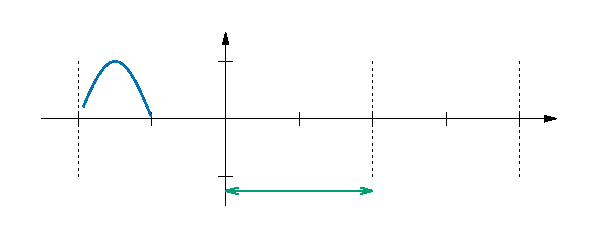
\includegraphics[width={273.60bp},height={100.70bp}]{figura_03_03}}%
    \gplfronttext
  \end{picture}%
\endgroup

\end{figure}

El periodo de la onda rectificada es el mismo que de la onda original.

\subsection{Rectificación de onda completa}
\begin{equation*}
    f(t)=A\,|\sen(\omega_0\,t)|
\end{equation*}
\begin{figure}[H]
    \centering
    % GNUPLOT: LaTeX picture with Postscript
\begingroup
  \makeatletter
  \providecommand\color[2][]{%
    \GenericError{(gnuplot) \space\space\space\@spaces}{%
      Package color not loaded in conjunction with
      terminal option `colourtext'%
    }{See the gnuplot documentation for explanation.%
    }{Either use 'blacktext' in gnuplot or load the package
      color.sty in LaTeX.}%
    \renewcommand\color[2][]{}%
  }%
  \providecommand\includegraphics[2][]{%
    \GenericError{(gnuplot) \space\space\space\@spaces}{%
      Package graphicx or graphics not loaded%
    }{See the gnuplot documentation for explanation.%
    }{The gnuplot epslatex terminal needs graphicx.sty or graphics.sty.}%
    \renewcommand\includegraphics[2][]{}%
  }%
  \providecommand\rotatebox[2]{#2}%
  \@ifundefined{ifGPcolor}{%
    \newif\ifGPcolor
    \GPcolorfalse
  }{}%
  \@ifundefined{ifGPblacktext}{%
    \newif\ifGPblacktext
    \GPblacktexttrue
  }{}%
  % define a \g@addto@macro without @ in the name:
  \let\gplgaddtomacro\g@addto@macro
  % define empty templates for all commands taking text:
  \gdef\gplbacktext{}%
  \gdef\gplfronttext{}%
  \makeatother
  \ifGPblacktext
    % no textcolor at all
    \def\colorrgb#1{}%
    \def\colorgray#1{}%
  \else
    % gray or color?
    \ifGPcolor
      \def\colorrgb#1{\color[rgb]{#1}}%
      \def\colorgray#1{\color[gray]{#1}}%
      \expandafter\def\csname LTw\endcsname{\color{white}}%
      \expandafter\def\csname LTb\endcsname{\color{black}}%
      \expandafter\def\csname LTa\endcsname{\color{black}}%
      \expandafter\def\csname LT0\endcsname{\color[rgb]{1,0,0}}%
      \expandafter\def\csname LT1\endcsname{\color[rgb]{0,1,0}}%
      \expandafter\def\csname LT2\endcsname{\color[rgb]{0,0,1}}%
      \expandafter\def\csname LT3\endcsname{\color[rgb]{1,0,1}}%
      \expandafter\def\csname LT4\endcsname{\color[rgb]{0,1,1}}%
      \expandafter\def\csname LT5\endcsname{\color[rgb]{1,1,0}}%
      \expandafter\def\csname LT6\endcsname{\color[rgb]{0,0,0}}%
      \expandafter\def\csname LT7\endcsname{\color[rgb]{1,0.3,0}}%
      \expandafter\def\csname LT8\endcsname{\color[rgb]{0.5,0.5,0.5}}%
    \else
      % gray
      \def\colorrgb#1{\color{black}}%
      \def\colorgray#1{\color[gray]{#1}}%
      \expandafter\def\csname LTw\endcsname{\color{white}}%
      \expandafter\def\csname LTb\endcsname{\color{black}}%
      \expandafter\def\csname LTa\endcsname{\color{black}}%
      \expandafter\def\csname LT0\endcsname{\color{black}}%
      \expandafter\def\csname LT1\endcsname{\color{black}}%
      \expandafter\def\csname LT2\endcsname{\color{black}}%
      \expandafter\def\csname LT3\endcsname{\color{black}}%
      \expandafter\def\csname LT4\endcsname{\color{black}}%
      \expandafter\def\csname LT5\endcsname{\color{black}}%
      \expandafter\def\csname LT6\endcsname{\color{black}}%
      \expandafter\def\csname LT7\endcsname{\color{black}}%
      \expandafter\def\csname LT8\endcsname{\color{black}}%
    \fi
  \fi
    \setlength{\unitlength}{0.0500bp}%
    \ifx\gptboxheight\undefined%
      \newlength{\gptboxheight}%
      \newlength{\gptboxwidth}%
      \newsavebox{\gptboxtext}%
    \fi%
    \setlength{\fboxrule}{0.5pt}%
    \setlength{\fboxsep}{1pt}%
    \definecolor{tbcol}{rgb}{1,1,1}%
\begin{picture}(5472.00,2014.00)%
    \gplgaddtomacro\gplbacktext{%
      \csname LTb\endcsname%%
      \put(1909,469){\makebox(0,0)[r]{\strut{}}}%
      \put(1909,1023){\makebox(0,0)[r]{\strut{}}}%
      \put(1909,1576){\makebox(0,0)[r]{\strut{}}}%
      \put(593,800){\makebox(0,0){\strut{}}}%
      \put(1299,800){\makebox(0,0){\strut{}}}%
      \put(2005,800){\makebox(0,0){\strut{}}}%
      \put(2712,800){\makebox(0,0){\strut{}}}%
      \put(3418,800){\makebox(0,0){\strut{}}}%
      \put(4124,800){\makebox(0,0){\strut{}}}%
      \put(4830,800){\makebox(0,0){\strut{}}}%
      \csname LTb\endcsname%%
      \put(5360,1023){\makebox(0,0)[l]{\strut{}$t$}}%
      \put(2005,1991){\makebox(0,0)[l]{\strut{}$f(t)$}}%
      \put(2330,137){\makebox(0,0)[l]{\strut{}$T$}}%
    }%
    \gplgaddtomacro\gplfronttext{%
    }%
    \gplgaddtomacro\gplbacktext{%
      \csname LTb\endcsname%%
      \put(1909,469){\makebox(0,0)[r]{\strut{}}}%
      \put(1909,1023){\makebox(0,0)[r]{\strut{}}}%
      \put(1909,1576){\makebox(0,0)[r]{\strut{}}}%
      \put(593,800){\makebox(0,0){\strut{}}}%
      \put(1299,800){\makebox(0,0){\strut{}}}%
      \put(2005,800){\makebox(0,0){\strut{}}}%
      \put(2712,800){\makebox(0,0){\strut{}}}%
      \put(3418,800){\makebox(0,0){\strut{}}}%
      \put(4124,800){\makebox(0,0){\strut{}}}%
      \put(4830,800){\makebox(0,0){\strut{}}}%
      \csname LTb\endcsname%%
      \put(5360,1023){\makebox(0,0)[l]{\strut{}$t$}}%
      \put(2005,1991){\makebox(0,0)[l]{\strut{}$f(t)$}}%
      \put(2330,137){\makebox(0,0)[l]{\strut{}$T$}}%
    }%
    \gplgaddtomacro\gplfronttext{%
    }%
    \gplgaddtomacro\gplbacktext{%
      \csname LTb\endcsname%%
      \put(1909,469){\makebox(0,0)[r]{\strut{}}}%
      \put(1909,1023){\makebox(0,0)[r]{\strut{}}}%
      \put(1909,1576){\makebox(0,0)[r]{\strut{}}}%
      \put(593,800){\makebox(0,0){\strut{}}}%
      \put(1299,800){\makebox(0,0){\strut{}}}%
      \put(2005,800){\makebox(0,0){\strut{}}}%
      \put(2712,800){\makebox(0,0){\strut{}}}%
      \put(3418,800){\makebox(0,0){\strut{}}}%
      \put(4124,800){\makebox(0,0){\strut{}}}%
      \put(4830,800){\makebox(0,0){\strut{}}}%
      \csname LTb\endcsname%%
      \put(5360,1023){\makebox(0,0)[l]{\strut{}$t$}}%
      \put(2005,1991){\makebox(0,0)[l]{\strut{}$f(t)$}}%
      \put(2330,137){\makebox(0,0)[l]{\strut{}$T$}}%
    }%
    \gplgaddtomacro\gplfronttext{%
    }%
    \gplgaddtomacro\gplbacktext{%
      \csname LTb\endcsname%%
      \put(1909,469){\makebox(0,0)[r]{\strut{}}}%
      \put(1909,1023){\makebox(0,0)[r]{\strut{}}}%
      \put(1909,1576){\makebox(0,0)[r]{\strut{}}}%
      \put(593,800){\makebox(0,0){\strut{}}}%
      \put(1299,800){\makebox(0,0){\strut{}}}%
      \put(2005,800){\makebox(0,0){\strut{}}}%
      \put(2712,800){\makebox(0,0){\strut{}}}%
      \put(3418,800){\makebox(0,0){\strut{}}}%
      \put(4124,800){\makebox(0,0){\strut{}}}%
      \put(4830,800){\makebox(0,0){\strut{}}}%
      \csname LTb\endcsname%%
      \put(5360,1023){\makebox(0,0)[l]{\strut{}$t$}}%
      \put(2005,1991){\makebox(0,0)[l]{\strut{}$f(t)$}}%
      \put(2330,137){\makebox(0,0)[l]{\strut{}$T$}}%
    }%
    \gplgaddtomacro\gplfronttext{%
    }%
    \gplgaddtomacro\gplbacktext{%
      \csname LTb\endcsname%%
      \put(1909,469){\makebox(0,0)[r]{\strut{}}}%
      \put(1909,1023){\makebox(0,0)[r]{\strut{}}}%
      \put(1909,1576){\makebox(0,0)[r]{\strut{}}}%
      \put(593,800){\makebox(0,0){\strut{}}}%
      \put(1299,800){\makebox(0,0){\strut{}}}%
      \put(2005,800){\makebox(0,0){\strut{}}}%
      \put(2712,800){\makebox(0,0){\strut{}}}%
      \put(3418,800){\makebox(0,0){\strut{}}}%
      \put(4124,800){\makebox(0,0){\strut{}}}%
      \put(4830,800){\makebox(0,0){\strut{}}}%
      \csname LTb\endcsname%%
      \put(5360,1023){\makebox(0,0)[l]{\strut{}$t$}}%
      \put(2005,1991){\makebox(0,0)[l]{\strut{}$f(t)$}}%
      \put(2330,137){\makebox(0,0)[l]{\strut{}$T$}}%
    }%
    \gplgaddtomacro\gplfronttext{%
    }%
    \gplgaddtomacro\gplbacktext{%
      \csname LTb\endcsname%%
      \put(1909,469){\makebox(0,0)[r]{\strut{}}}%
      \put(1909,1023){\makebox(0,0)[r]{\strut{}}}%
      \put(1909,1576){\makebox(0,0)[r]{\strut{}}}%
      \put(593,800){\makebox(0,0){\strut{}}}%
      \put(1299,800){\makebox(0,0){\strut{}}}%
      \put(2005,800){\makebox(0,0){\strut{}}}%
      \put(2712,800){\makebox(0,0){\strut{}}}%
      \put(3418,800){\makebox(0,0){\strut{}}}%
      \put(4124,800){\makebox(0,0){\strut{}}}%
      \put(4830,800){\makebox(0,0){\strut{}}}%
      \csname LTb\endcsname%%
      \put(5360,1023){\makebox(0,0)[l]{\strut{}$t$}}%
      \put(2005,1991){\makebox(0,0)[l]{\strut{}$f(t)$}}%
      \put(2330,137){\makebox(0,0)[l]{\strut{}$T$}}%
    }%
    \gplgaddtomacro\gplfronttext{%
    }%
    \gplgaddtomacro\gplbacktext{%
      \csname LTb\endcsname%%
      \put(1909,469){\makebox(0,0)[r]{\strut{}}}%
      \put(1909,1023){\makebox(0,0)[r]{\strut{}}}%
      \put(1909,1576){\makebox(0,0)[r]{\strut{}}}%
      \put(593,800){\makebox(0,0){\strut{}}}%
      \put(1299,800){\makebox(0,0){\strut{}}}%
      \put(2005,800){\makebox(0,0){\strut{}}}%
      \put(2712,800){\makebox(0,0){\strut{}}}%
      \put(3418,800){\makebox(0,0){\strut{}}}%
      \put(4124,800){\makebox(0,0){\strut{}}}%
      \put(4830,800){\makebox(0,0){\strut{}}}%
      \csname LTb\endcsname%%
      \put(5360,1023){\makebox(0,0)[l]{\strut{}$t$}}%
      \put(2005,1991){\makebox(0,0)[l]{\strut{}$f(t)$}}%
      \put(2330,137){\makebox(0,0)[l]{\strut{}$T$}}%
    }%
    \gplgaddtomacro\gplfronttext{%
    }%
    \gplgaddtomacro\gplbacktext{%
      \csname LTb\endcsname%%
      \put(1909,469){\makebox(0,0)[r]{\strut{}}}%
      \put(1909,1023){\makebox(0,0)[r]{\strut{}}}%
      \put(1909,1576){\makebox(0,0)[r]{\strut{}}}%
      \put(593,800){\makebox(0,0){\strut{}}}%
      \put(1299,800){\makebox(0,0){\strut{}}}%
      \put(2005,800){\makebox(0,0){\strut{}}}%
      \put(2712,800){\makebox(0,0){\strut{}}}%
      \put(3418,800){\makebox(0,0){\strut{}}}%
      \put(4124,800){\makebox(0,0){\strut{}}}%
      \put(4830,800){\makebox(0,0){\strut{}}}%
      \csname LTb\endcsname%%
      \put(5360,1023){\makebox(0,0)[l]{\strut{}$t$}}%
      \put(2005,1991){\makebox(0,0)[l]{\strut{}$f(t)$}}%
      \put(2330,137){\makebox(0,0)[l]{\strut{}$T$}}%
    }%
    \gplgaddtomacro\gplfronttext{%
    }%
    \gplgaddtomacro\gplbacktext{%
      \csname LTb\endcsname%%
      \put(1909,469){\makebox(0,0)[r]{\strut{}}}%
      \put(1909,1023){\makebox(0,0)[r]{\strut{}}}%
      \put(1909,1576){\makebox(0,0)[r]{\strut{}}}%
      \put(593,800){\makebox(0,0){\strut{}}}%
      \put(1299,800){\makebox(0,0){\strut{}}}%
      \put(2005,800){\makebox(0,0){\strut{}}}%
      \put(2712,800){\makebox(0,0){\strut{}}}%
      \put(3418,800){\makebox(0,0){\strut{}}}%
      \put(4124,800){\makebox(0,0){\strut{}}}%
      \put(4830,800){\makebox(0,0){\strut{}}}%
      \csname LTb\endcsname%%
      \put(5360,1023){\makebox(0,0)[l]{\strut{}$t$}}%
      \put(2005,1991){\makebox(0,0)[l]{\strut{}$f(t)$}}%
      \put(2330,137){\makebox(0,0)[l]{\strut{}$T$}}%
    }%
    \gplgaddtomacro\gplfronttext{%
    }%
    \gplbacktext
    \put(0,0){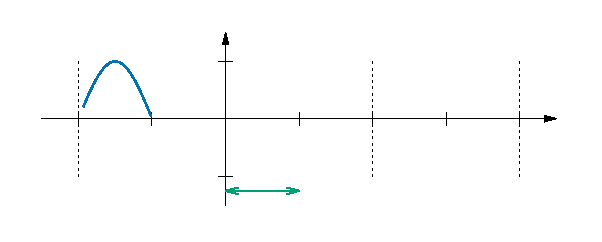
\includegraphics[width={273.60bp},height={100.70bp}]{figura_03_04}}%
    \gplfronttext
  \end{picture}%
\endgroup

\end{figure}

El periodo de la onda rectificada es la mitad del periodo de la onda original.

\section{Función escalón unitario}
\begin{equation}
    u(t)=\begin{cases}
        0&t<0\\
        1&t>0\\
    \end{cases}
\end{equation}
\begin{figure}[H]
    \centering
    % GNUPLOT: LaTeX picture with Postscript
\begingroup
  \makeatletter
  \providecommand\color[2][]{%
    \GenericError{(gnuplot) \space\space\space\@spaces}{%
      Package color not loaded in conjunction with
      terminal option `colourtext'%
    }{See the gnuplot documentation for explanation.%
    }{Either use 'blacktext' in gnuplot or load the package
      color.sty in LaTeX.}%
    \renewcommand\color[2][]{}%
  }%
  \providecommand\includegraphics[2][]{%
    \GenericError{(gnuplot) \space\space\space\@spaces}{%
      Package graphicx or graphics not loaded%
    }{See the gnuplot documentation for explanation.%
    }{The gnuplot epslatex terminal needs graphicx.sty or graphics.sty.}%
    \renewcommand\includegraphics[2][]{}%
  }%
  \providecommand\rotatebox[2]{#2}%
  \@ifundefined{ifGPcolor}{%
    \newif\ifGPcolor
    \GPcolorfalse
  }{}%
  \@ifundefined{ifGPblacktext}{%
    \newif\ifGPblacktext
    \GPblacktexttrue
  }{}%
  % define a \g@addto@macro without @ in the name:
  \let\gplgaddtomacro\g@addto@macro
  % define empty templates for all commands taking text:
  \gdef\gplbacktext{}%
  \gdef\gplfronttext{}%
  \makeatother
  \ifGPblacktext
    % no textcolor at all
    \def\colorrgb#1{}%
    \def\colorgray#1{}%
  \else
    % gray or color?
    \ifGPcolor
      \def\colorrgb#1{\color[rgb]{#1}}%
      \def\colorgray#1{\color[gray]{#1}}%
      \expandafter\def\csname LTw\endcsname{\color{white}}%
      \expandafter\def\csname LTb\endcsname{\color{black}}%
      \expandafter\def\csname LTa\endcsname{\color{black}}%
      \expandafter\def\csname LT0\endcsname{\color[rgb]{1,0,0}}%
      \expandafter\def\csname LT1\endcsname{\color[rgb]{0,1,0}}%
      \expandafter\def\csname LT2\endcsname{\color[rgb]{0,0,1}}%
      \expandafter\def\csname LT3\endcsname{\color[rgb]{1,0,1}}%
      \expandafter\def\csname LT4\endcsname{\color[rgb]{0,1,1}}%
      \expandafter\def\csname LT5\endcsname{\color[rgb]{1,1,0}}%
      \expandafter\def\csname LT6\endcsname{\color[rgb]{0,0,0}}%
      \expandafter\def\csname LT7\endcsname{\color[rgb]{1,0.3,0}}%
      \expandafter\def\csname LT8\endcsname{\color[rgb]{0.5,0.5,0.5}}%
    \else
      % gray
      \def\colorrgb#1{\color{black}}%
      \def\colorgray#1{\color[gray]{#1}}%
      \expandafter\def\csname LTw\endcsname{\color{white}}%
      \expandafter\def\csname LTb\endcsname{\color{black}}%
      \expandafter\def\csname LTa\endcsname{\color{black}}%
      \expandafter\def\csname LT0\endcsname{\color{black}}%
      \expandafter\def\csname LT1\endcsname{\color{black}}%
      \expandafter\def\csname LT2\endcsname{\color{black}}%
      \expandafter\def\csname LT3\endcsname{\color{black}}%
      \expandafter\def\csname LT4\endcsname{\color{black}}%
      \expandafter\def\csname LT5\endcsname{\color{black}}%
      \expandafter\def\csname LT6\endcsname{\color{black}}%
      \expandafter\def\csname LT7\endcsname{\color{black}}%
      \expandafter\def\csname LT8\endcsname{\color{black}}%
    \fi
  \fi
    \setlength{\unitlength}{0.0500bp}%
    \ifx\gptboxheight\undefined%
      \newlength{\gptboxheight}%
      \newlength{\gptboxwidth}%
      \newsavebox{\gptboxtext}%
    \fi%
    \setlength{\fboxrule}{0.5pt}%
    \setlength{\fboxsep}{1pt}%
    \definecolor{tbcol}{rgb}{1,1,1}%
\begin{picture}(5760.00,1440.00)%
    \gplgaddtomacro\gplbacktext{%
      \csname LTb\endcsname%%
      \put(2760,464){\makebox(0,0)[r]{\strut{}}}%
      \put(2760,1007){\makebox(0,0)[r]{\strut{}}}%
      \put(240,241){\makebox(0,0){\strut{}}}%
      \put(763,241){\makebox(0,0){\strut{}}}%
      \put(1286,241){\makebox(0,0){\strut{}}}%
      \put(1809,241){\makebox(0,0){\strut{}}}%
      \put(2332,241){\makebox(0,0){\strut{}}}%
      \put(2856,241){\makebox(0,0){\strut{}}}%
      \put(3379,241){\makebox(0,0){\strut{}}}%
      \put(3902,241){\makebox(0,0){\strut{}}}%
      \put(4425,241){\makebox(0,0){\strut{}}}%
      \put(4948,241){\makebox(0,0){\strut{}}}%
      \put(5471,241){\makebox(0,0){\strut{}}}%
      \csname LTb\endcsname%%
      \put(6256,464){\makebox(0,0)[l]{\strut{}$t$}}%
      \put(2751,1496){\makebox(0,0)[l]{\strut{}$f(t)$}}%
      \put(2594,1007){\makebox(0,0)[l]{\strut{}$1$}}%
    }%
    \gplgaddtomacro\gplfronttext{%
    }%
    \gplbacktext
    \put(0,0){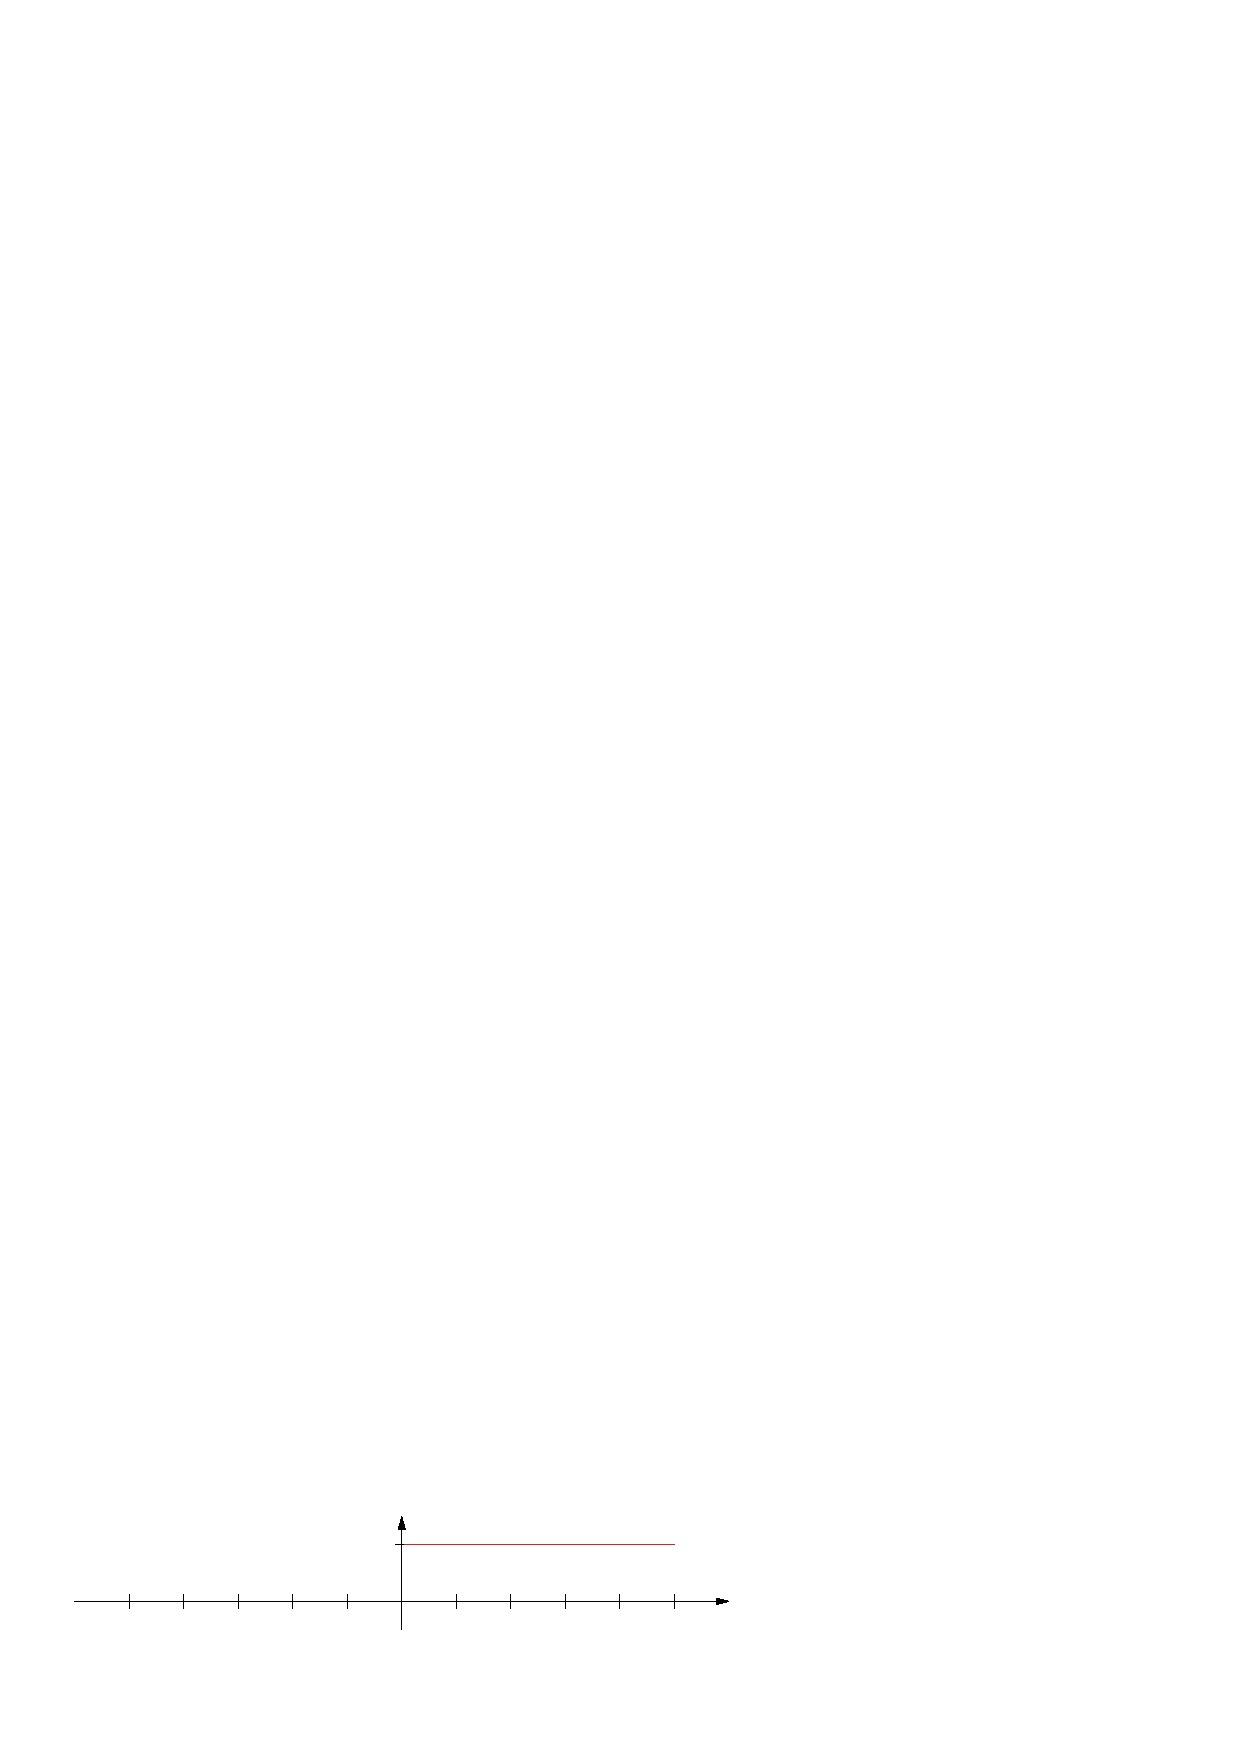
\includegraphics[width={288.00bp},height={72.00bp}]{figura_03_05}}%
    \gplfronttext
  \end{picture}%
\endgroup

\end{figure}

Una variante es:
\begin{equation*}
    u(-t)=\begin{cases}
        1&t<0\\
        0&t>0\\
    \end{cases}
\end{equation*}
\begin{figure}[H]
    \centering
    % GNUPLOT: LaTeX picture with Postscript
\begingroup
  \makeatletter
  \providecommand\color[2][]{%
    \GenericError{(gnuplot) \space\space\space\@spaces}{%
      Package color not loaded in conjunction with
      terminal option `colourtext'%
    }{See the gnuplot documentation for explanation.%
    }{Either use 'blacktext' in gnuplot or load the package
      color.sty in LaTeX.}%
    \renewcommand\color[2][]{}%
  }%
  \providecommand\includegraphics[2][]{%
    \GenericError{(gnuplot) \space\space\space\@spaces}{%
      Package graphicx or graphics not loaded%
    }{See the gnuplot documentation for explanation.%
    }{The gnuplot epslatex terminal needs graphicx.sty or graphics.sty.}%
    \renewcommand\includegraphics[2][]{}%
  }%
  \providecommand\rotatebox[2]{#2}%
  \@ifundefined{ifGPcolor}{%
    \newif\ifGPcolor
    \GPcolorfalse
  }{}%
  \@ifundefined{ifGPblacktext}{%
    \newif\ifGPblacktext
    \GPblacktexttrue
  }{}%
  % define a \g@addto@macro without @ in the name:
  \let\gplgaddtomacro\g@addto@macro
  % define empty templates for all commands taking text:
  \gdef\gplbacktext{}%
  \gdef\gplfronttext{}%
  \makeatother
  \ifGPblacktext
    % no textcolor at all
    \def\colorrgb#1{}%
    \def\colorgray#1{}%
  \else
    % gray or color?
    \ifGPcolor
      \def\colorrgb#1{\color[rgb]{#1}}%
      \def\colorgray#1{\color[gray]{#1}}%
      \expandafter\def\csname LTw\endcsname{\color{white}}%
      \expandafter\def\csname LTb\endcsname{\color{black}}%
      \expandafter\def\csname LTa\endcsname{\color{black}}%
      \expandafter\def\csname LT0\endcsname{\color[rgb]{1,0,0}}%
      \expandafter\def\csname LT1\endcsname{\color[rgb]{0,1,0}}%
      \expandafter\def\csname LT2\endcsname{\color[rgb]{0,0,1}}%
      \expandafter\def\csname LT3\endcsname{\color[rgb]{1,0,1}}%
      \expandafter\def\csname LT4\endcsname{\color[rgb]{0,1,1}}%
      \expandafter\def\csname LT5\endcsname{\color[rgb]{1,1,0}}%
      \expandafter\def\csname LT6\endcsname{\color[rgb]{0,0,0}}%
      \expandafter\def\csname LT7\endcsname{\color[rgb]{1,0.3,0}}%
      \expandafter\def\csname LT8\endcsname{\color[rgb]{0.5,0.5,0.5}}%
    \else
      % gray
      \def\colorrgb#1{\color{black}}%
      \def\colorgray#1{\color[gray]{#1}}%
      \expandafter\def\csname LTw\endcsname{\color{white}}%
      \expandafter\def\csname LTb\endcsname{\color{black}}%
      \expandafter\def\csname LTa\endcsname{\color{black}}%
      \expandafter\def\csname LT0\endcsname{\color{black}}%
      \expandafter\def\csname LT1\endcsname{\color{black}}%
      \expandafter\def\csname LT2\endcsname{\color{black}}%
      \expandafter\def\csname LT3\endcsname{\color{black}}%
      \expandafter\def\csname LT4\endcsname{\color{black}}%
      \expandafter\def\csname LT5\endcsname{\color{black}}%
      \expandafter\def\csname LT6\endcsname{\color{black}}%
      \expandafter\def\csname LT7\endcsname{\color{black}}%
      \expandafter\def\csname LT8\endcsname{\color{black}}%
    \fi
  \fi
    \setlength{\unitlength}{0.0500bp}%
    \ifx\gptboxheight\undefined%
      \newlength{\gptboxheight}%
      \newlength{\gptboxwidth}%
      \newsavebox{\gptboxtext}%
    \fi%
    \setlength{\fboxrule}{0.5pt}%
    \setlength{\fboxsep}{1pt}%
    \definecolor{tbcol}{rgb}{1,1,1}%
\begin{picture}(5760.00,1440.00)%
    \gplgaddtomacro\gplbacktext{%
      \csname LTb\endcsname%%
      \put(2760,464){\makebox(0,0)[r]{\strut{}}}%
      \put(2760,1007){\makebox(0,0)[r]{\strut{}}}%
      \put(240,241){\makebox(0,0){\strut{}}}%
      \put(763,241){\makebox(0,0){\strut{}}}%
      \put(1286,241){\makebox(0,0){\strut{}}}%
      \put(1809,241){\makebox(0,0){\strut{}}}%
      \put(2332,241){\makebox(0,0){\strut{}}}%
      \put(2856,241){\makebox(0,0){\strut{}}}%
      \put(3379,241){\makebox(0,0){\strut{}}}%
      \put(3902,241){\makebox(0,0){\strut{}}}%
      \put(4425,241){\makebox(0,0){\strut{}}}%
      \put(4948,241){\makebox(0,0){\strut{}}}%
      \put(5471,241){\makebox(0,0){\strut{}}}%
      \csname LTb\endcsname%%
      \put(6256,464){\makebox(0,0)[l]{\strut{}$t$}}%
      \put(2751,1496){\makebox(0,0)[l]{\strut{}$f(t)$}}%
      \put(3012,1007){\makebox(0,0)[l]{\strut{}$1$}}%
    }%
    \gplgaddtomacro\gplfronttext{%
    }%
    \gplbacktext
    \put(0,0){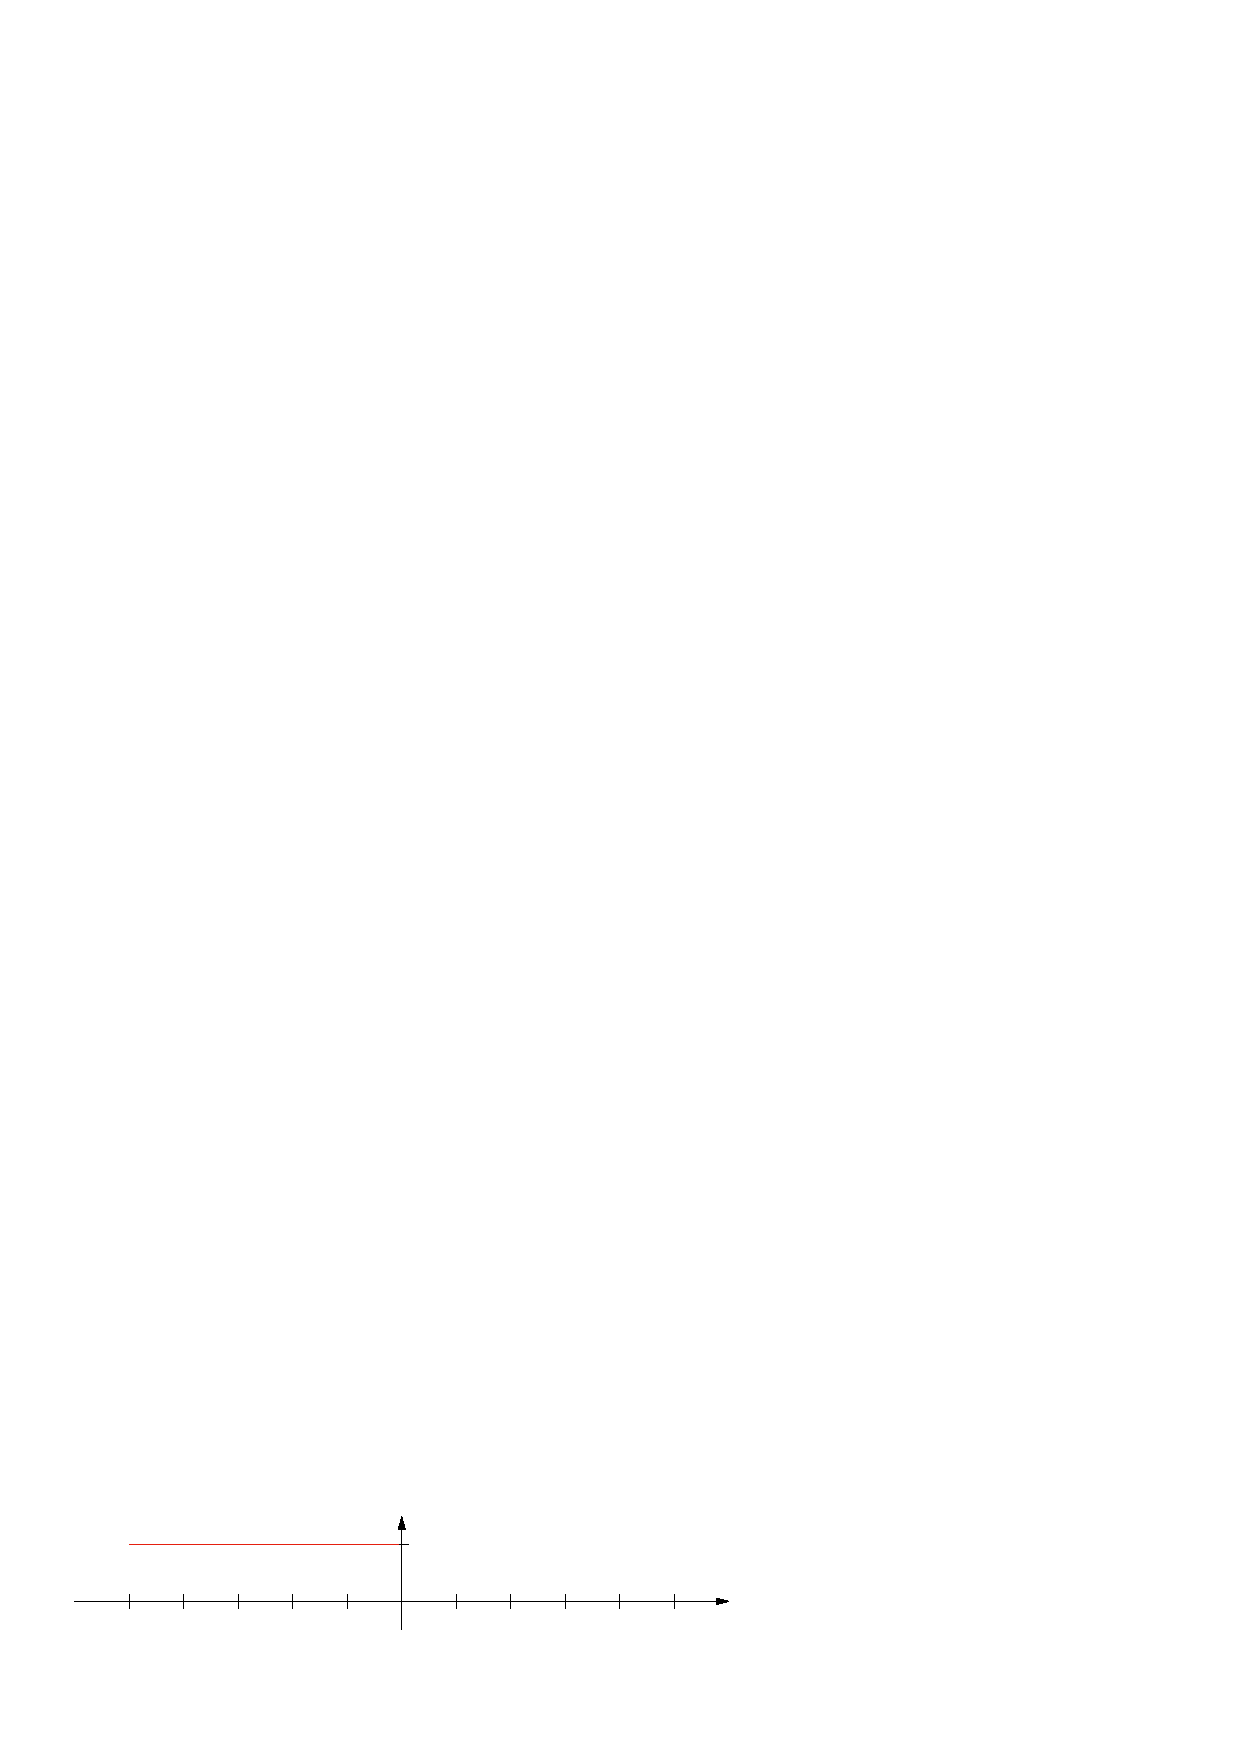
\includegraphics[width={288.00bp},height={72.00bp}]{figura_03_06}}%
    \gplfronttext
  \end{picture}%
\endgroup

\end{figure}

De manera general:
\begin{equation}
    k\,u(t-t_0)=\begin{cases}
        0&t<t_0\\
        k&t>t_0\\
    \end{cases}
\end{equation}
\begin{figure}[H]
    \centering
    % GNUPLOT: LaTeX picture with Postscript
\begingroup
  \makeatletter
  \providecommand\color[2][]{%
    \GenericError{(gnuplot) \space\space\space\@spaces}{%
      Package color not loaded in conjunction with
      terminal option `colourtext'%
    }{See the gnuplot documentation for explanation.%
    }{Either use 'blacktext' in gnuplot or load the package
      color.sty in LaTeX.}%
    \renewcommand\color[2][]{}%
  }%
  \providecommand\includegraphics[2][]{%
    \GenericError{(gnuplot) \space\space\space\@spaces}{%
      Package graphicx or graphics not loaded%
    }{See the gnuplot documentation for explanation.%
    }{The gnuplot epslatex terminal needs graphicx.sty or graphics.sty.}%
    \renewcommand\includegraphics[2][]{}%
  }%
  \providecommand\rotatebox[2]{#2}%
  \@ifundefined{ifGPcolor}{%
    \newif\ifGPcolor
    \GPcolorfalse
  }{}%
  \@ifundefined{ifGPblacktext}{%
    \newif\ifGPblacktext
    \GPblacktexttrue
  }{}%
  % define a \g@addto@macro without @ in the name:
  \let\gplgaddtomacro\g@addto@macro
  % define empty templates for all commands taking text:
  \gdef\gplbacktext{}%
  \gdef\gplfronttext{}%
  \makeatother
  \ifGPblacktext
    % no textcolor at all
    \def\colorrgb#1{}%
    \def\colorgray#1{}%
  \else
    % gray or color?
    \ifGPcolor
      \def\colorrgb#1{\color[rgb]{#1}}%
      \def\colorgray#1{\color[gray]{#1}}%
      \expandafter\def\csname LTw\endcsname{\color{white}}%
      \expandafter\def\csname LTb\endcsname{\color{black}}%
      \expandafter\def\csname LTa\endcsname{\color{black}}%
      \expandafter\def\csname LT0\endcsname{\color[rgb]{1,0,0}}%
      \expandafter\def\csname LT1\endcsname{\color[rgb]{0,1,0}}%
      \expandafter\def\csname LT2\endcsname{\color[rgb]{0,0,1}}%
      \expandafter\def\csname LT3\endcsname{\color[rgb]{1,0,1}}%
      \expandafter\def\csname LT4\endcsname{\color[rgb]{0,1,1}}%
      \expandafter\def\csname LT5\endcsname{\color[rgb]{1,1,0}}%
      \expandafter\def\csname LT6\endcsname{\color[rgb]{0,0,0}}%
      \expandafter\def\csname LT7\endcsname{\color[rgb]{1,0.3,0}}%
      \expandafter\def\csname LT8\endcsname{\color[rgb]{0.5,0.5,0.5}}%
    \else
      % gray
      \def\colorrgb#1{\color{black}}%
      \def\colorgray#1{\color[gray]{#1}}%
      \expandafter\def\csname LTw\endcsname{\color{white}}%
      \expandafter\def\csname LTb\endcsname{\color{black}}%
      \expandafter\def\csname LTa\endcsname{\color{black}}%
      \expandafter\def\csname LT0\endcsname{\color{black}}%
      \expandafter\def\csname LT1\endcsname{\color{black}}%
      \expandafter\def\csname LT2\endcsname{\color{black}}%
      \expandafter\def\csname LT3\endcsname{\color{black}}%
      \expandafter\def\csname LT4\endcsname{\color{black}}%
      \expandafter\def\csname LT5\endcsname{\color{black}}%
      \expandafter\def\csname LT6\endcsname{\color{black}}%
      \expandafter\def\csname LT7\endcsname{\color{black}}%
      \expandafter\def\csname LT8\endcsname{\color{black}}%
    \fi
  \fi
    \setlength{\unitlength}{0.0500bp}%
    \ifx\gptboxheight\undefined%
      \newlength{\gptboxheight}%
      \newlength{\gptboxwidth}%
      \newsavebox{\gptboxtext}%
    \fi%
    \setlength{\fboxrule}{0.5pt}%
    \setlength{\fboxsep}{1pt}%
    \definecolor{tbcol}{rgb}{1,1,1}%
\begin{picture}(5760.00,2160.00)%
    \gplgaddtomacro\gplbacktext{%
      \csname LTb\endcsname%%
      \put(2760,493){\makebox(0,0)[r]{\strut{}}}%
      \put(2760,1096){\makebox(0,0)[r]{\strut{}}}%
      \put(2760,1698){\makebox(0,0)[r]{\strut{}}}%
      \put(240,270){\makebox(0,0){\strut{}}}%
      \put(763,270){\makebox(0,0){\strut{}}}%
      \put(1286,270){\makebox(0,0){\strut{}}}%
      \put(1809,270){\makebox(0,0){\strut{}}}%
      \put(2332,270){\makebox(0,0){\strut{}}}%
      \put(2856,270){\makebox(0,0){\strut{}}}%
      \put(3379,270){\makebox(0,0){\strut{}}}%
      \put(3902,270){\makebox(0,0){\strut{}}}%
      \put(4425,270){\makebox(0,0){\strut{}}}%
      \put(4948,270){\makebox(0,0){\strut{}}}%
      \put(5471,270){\makebox(0,0){\strut{}}}%
      \csname LTb\endcsname%%
      \put(6256,493){\makebox(0,0)[l]{\strut{}$t$}}%
      \put(2751,2240){\makebox(0,0)[l]{\strut{}$f(t)$}}%
      \put(3588,312){\makebox(0,0)[l]{\strut{}$t_0$}}%
      \put(2594,1397){\makebox(0,0)[l]{\strut{}$k$}}%
    }%
    \gplgaddtomacro\gplfronttext{%
    }%
    \gplbacktext
    \put(0,0){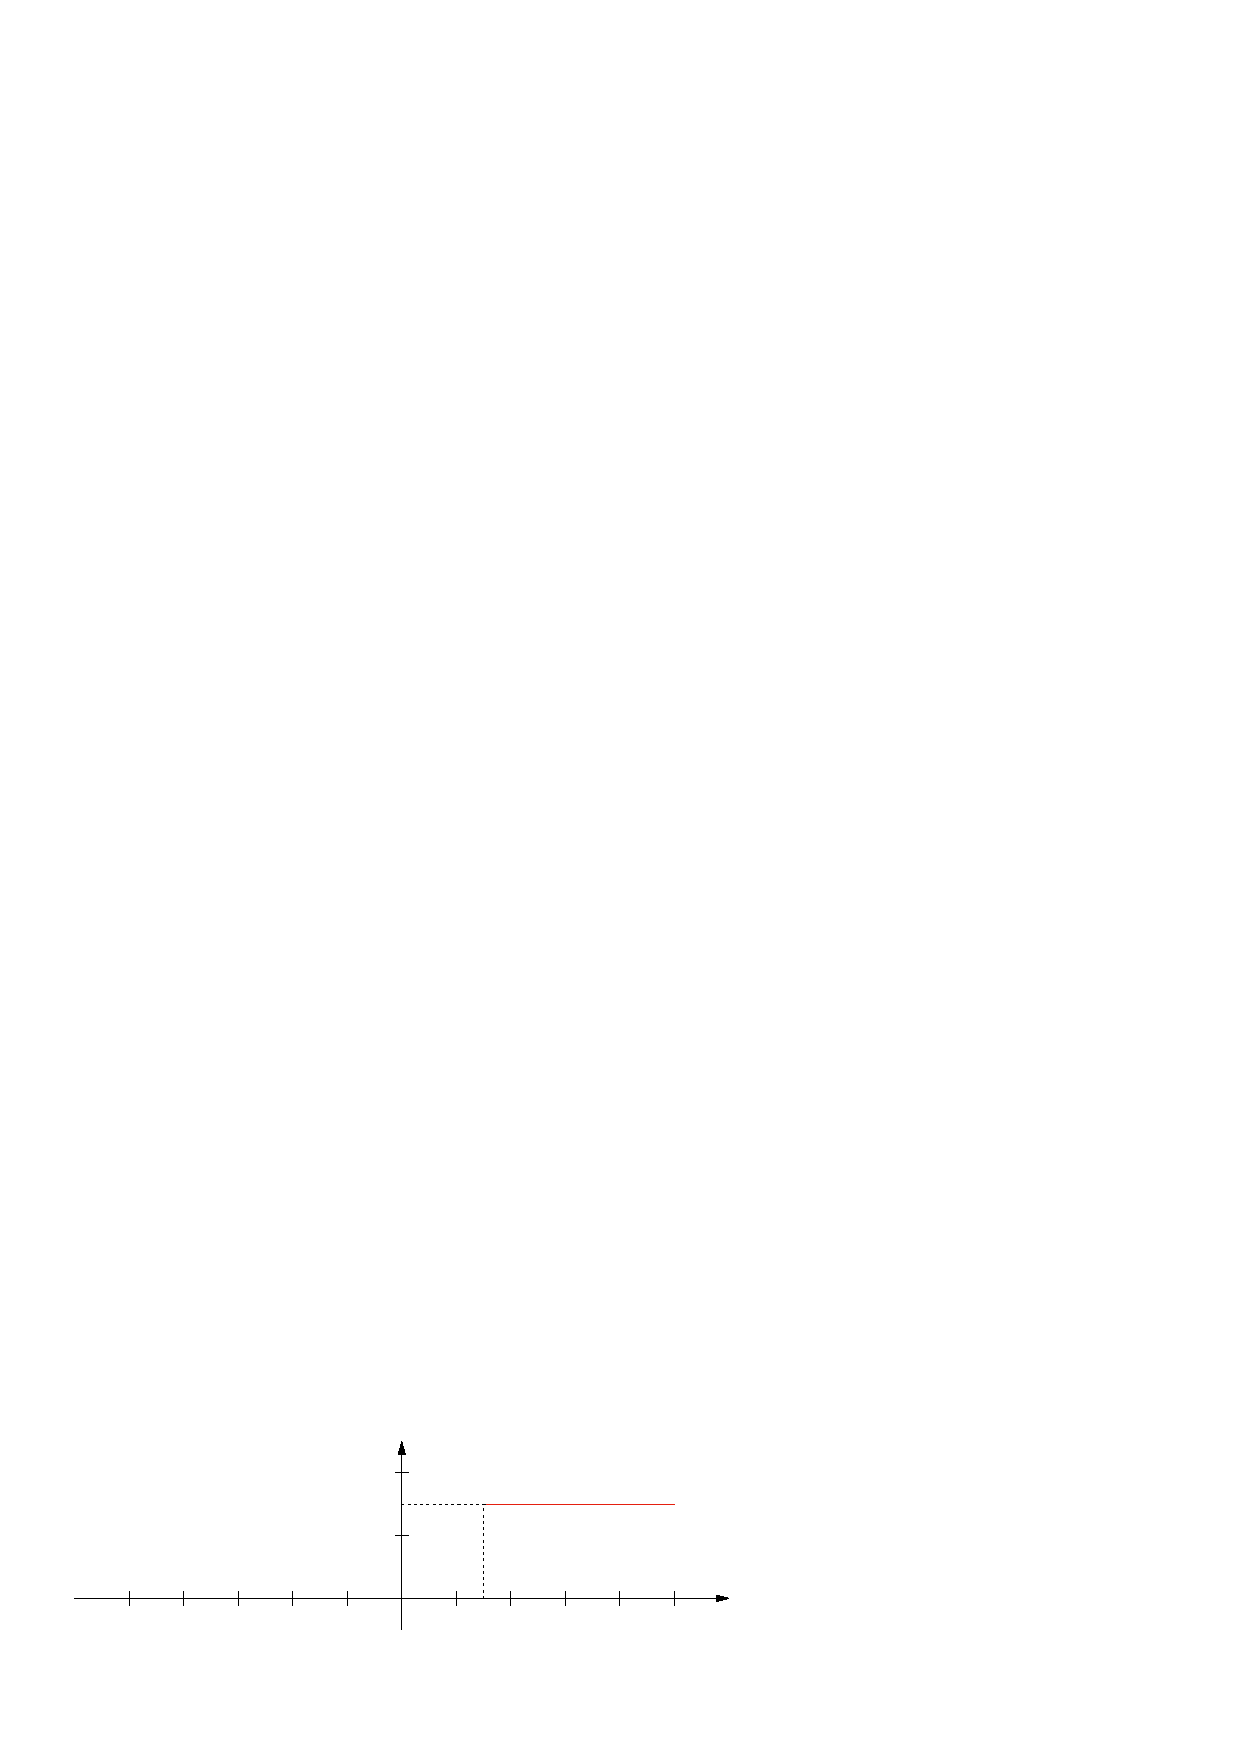
\includegraphics[width={288.00bp},height={108.00bp}]{figura_03_07}}%
    \gplfronttext
  \end{picture}%
\endgroup

\end{figure}

Si: $\phi(t)$ es una función de prueba:
\begin{figure}[H]
    \centering
    % GNUPLOT: LaTeX picture with Postscript
\begingroup
  \makeatletter
  \providecommand\color[2][]{%
    \GenericError{(gnuplot) \space\space\space\@spaces}{%
      Package color not loaded in conjunction with
      terminal option `colourtext'%
    }{See the gnuplot documentation for explanation.%
    }{Either use 'blacktext' in gnuplot or load the package
      color.sty in LaTeX.}%
    \renewcommand\color[2][]{}%
  }%
  \providecommand\includegraphics[2][]{%
    \GenericError{(gnuplot) \space\space\space\@spaces}{%
      Package graphicx or graphics not loaded%
    }{See the gnuplot documentation for explanation.%
    }{The gnuplot epslatex terminal needs graphicx.sty or graphics.sty.}%
    \renewcommand\includegraphics[2][]{}%
  }%
  \providecommand\rotatebox[2]{#2}%
  \@ifundefined{ifGPcolor}{%
    \newif\ifGPcolor
    \GPcolorfalse
  }{}%
  \@ifundefined{ifGPblacktext}{%
    \newif\ifGPblacktext
    \GPblacktexttrue
  }{}%
  % define a \g@addto@macro without @ in the name:
  \let\gplgaddtomacro\g@addto@macro
  % define empty templates for all commands taking text:
  \gdef\gplbacktext{}%
  \gdef\gplfronttext{}%
  \makeatother
  \ifGPblacktext
    % no textcolor at all
    \def\colorrgb#1{}%
    \def\colorgray#1{}%
  \else
    % gray or color?
    \ifGPcolor
      \def\colorrgb#1{\color[rgb]{#1}}%
      \def\colorgray#1{\color[gray]{#1}}%
      \expandafter\def\csname LTw\endcsname{\color{white}}%
      \expandafter\def\csname LTb\endcsname{\color{black}}%
      \expandafter\def\csname LTa\endcsname{\color{black}}%
      \expandafter\def\csname LT0\endcsname{\color[rgb]{1,0,0}}%
      \expandafter\def\csname LT1\endcsname{\color[rgb]{0,1,0}}%
      \expandafter\def\csname LT2\endcsname{\color[rgb]{0,0,1}}%
      \expandafter\def\csname LT3\endcsname{\color[rgb]{1,0,1}}%
      \expandafter\def\csname LT4\endcsname{\color[rgb]{0,1,1}}%
      \expandafter\def\csname LT5\endcsname{\color[rgb]{1,1,0}}%
      \expandafter\def\csname LT6\endcsname{\color[rgb]{0,0,0}}%
      \expandafter\def\csname LT7\endcsname{\color[rgb]{1,0.3,0}}%
      \expandafter\def\csname LT8\endcsname{\color[rgb]{0.5,0.5,0.5}}%
    \else
      % gray
      \def\colorrgb#1{\color{black}}%
      \def\colorgray#1{\color[gray]{#1}}%
      \expandafter\def\csname LTw\endcsname{\color{white}}%
      \expandafter\def\csname LTb\endcsname{\color{black}}%
      \expandafter\def\csname LTa\endcsname{\color{black}}%
      \expandafter\def\csname LT0\endcsname{\color{black}}%
      \expandafter\def\csname LT1\endcsname{\color{black}}%
      \expandafter\def\csname LT2\endcsname{\color{black}}%
      \expandafter\def\csname LT3\endcsname{\color{black}}%
      \expandafter\def\csname LT4\endcsname{\color{black}}%
      \expandafter\def\csname LT5\endcsname{\color{black}}%
      \expandafter\def\csname LT6\endcsname{\color{black}}%
      \expandafter\def\csname LT7\endcsname{\color{black}}%
      \expandafter\def\csname LT8\endcsname{\color{black}}%
    \fi
  \fi
    \setlength{\unitlength}{0.0500bp}%
    \ifx\gptboxheight\undefined%
      \newlength{\gptboxheight}%
      \newlength{\gptboxwidth}%
      \newsavebox{\gptboxtext}%
    \fi%
    \setlength{\fboxrule}{0.5pt}%
    \setlength{\fboxsep}{1pt}%
    \definecolor{tbcol}{rgb}{1,1,1}%
\begin{picture}(4320.00,2880.00)%
    \gplgaddtomacro\gplbacktext{%
      \csname LTb\endcsname%%
      \put(2040,192){\makebox(0,0)[r]{\strut{}}}%
      \put(2040,553){\makebox(0,0)[r]{\strut{}}}%
      \put(2040,914){\makebox(0,0)[r]{\strut{}}}%
      \put(2040,1275){\makebox(0,0)[r]{\strut{}}}%
      \put(2040,1636){\makebox(0,0)[r]{\strut{}}}%
      \put(2040,1997){\makebox(0,0)[r]{\strut{}}}%
      \put(2040,2358){\makebox(0,0)[r]{\strut{}}}%
      \put(2040,2719){\makebox(0,0)[r]{\strut{}}}%
      \put(240,330){\makebox(0,0){\strut{}}}%
      \put(714,330){\makebox(0,0){\strut{}}}%
      \put(1188,330){\makebox(0,0){\strut{}}}%
      \put(1662,330){\makebox(0,0){\strut{}}}%
      \put(2136,330){\makebox(0,0){\strut{}}}%
      \put(2609,330){\makebox(0,0){\strut{}}}%
      \put(3083,330){\makebox(0,0){\strut{}}}%
      \put(3557,330){\makebox(0,0){\strut{}}}%
      \put(4031,330){\makebox(0,0){\strut{}}}%
      \csname LTb\endcsname%%
      \put(4647,553){\makebox(0,0)[l]{\strut{}$t$}}%
      \put(2349,2863){\makebox(0,0)[l]{\strut{}$f(t)$}}%
      \put(2562,336){\makebox(0,0)[l]{\strut{}$t_0$}}%
      \put(1851,914){\makebox(0,0)[l]{\strut{}$1$}}%
      \put(714,2178){\makebox(0,0)[l]{\strut{}$\phi(t)$}}%
      \put(3083,1095){\makebox(0,0)[l]{\strut{}$u(t-t_0)$}}%
    }%
    \gplgaddtomacro\gplfronttext{%
    }%
    \gplgaddtomacro\gplbacktext{%
      \csname LTb\endcsname%%
      \put(2040,192){\makebox(0,0)[r]{\strut{}}}%
      \put(2040,553){\makebox(0,0)[r]{\strut{}}}%
      \put(2040,914){\makebox(0,0)[r]{\strut{}}}%
      \put(2040,1275){\makebox(0,0)[r]{\strut{}}}%
      \put(2040,1636){\makebox(0,0)[r]{\strut{}}}%
      \put(2040,1997){\makebox(0,0)[r]{\strut{}}}%
      \put(2040,2358){\makebox(0,0)[r]{\strut{}}}%
      \put(2040,2719){\makebox(0,0)[r]{\strut{}}}%
      \put(240,330){\makebox(0,0){\strut{}}}%
      \put(714,330){\makebox(0,0){\strut{}}}%
      \put(1188,330){\makebox(0,0){\strut{}}}%
      \put(1662,330){\makebox(0,0){\strut{}}}%
      \put(2136,330){\makebox(0,0){\strut{}}}%
      \put(2609,330){\makebox(0,0){\strut{}}}%
      \put(3083,330){\makebox(0,0){\strut{}}}%
      \put(3557,330){\makebox(0,0){\strut{}}}%
      \put(4031,330){\makebox(0,0){\strut{}}}%
      \csname LTb\endcsname%%
      \put(4647,553){\makebox(0,0)[l]{\strut{}$t$}}%
      \put(2349,2863){\makebox(0,0)[l]{\strut{}$f(t)$}}%
      \put(2562,336){\makebox(0,0)[l]{\strut{}$t_0$}}%
      \put(1851,914){\makebox(0,0)[l]{\strut{}$1$}}%
      \put(714,2178){\makebox(0,0)[l]{\strut{}$\phi(t)$}}%
      \put(3083,1095){\makebox(0,0)[l]{\strut{}$u(t-t_0)$}}%
    }%
    \gplgaddtomacro\gplfronttext{%
    }%
    \gplbacktext
    \put(0,0){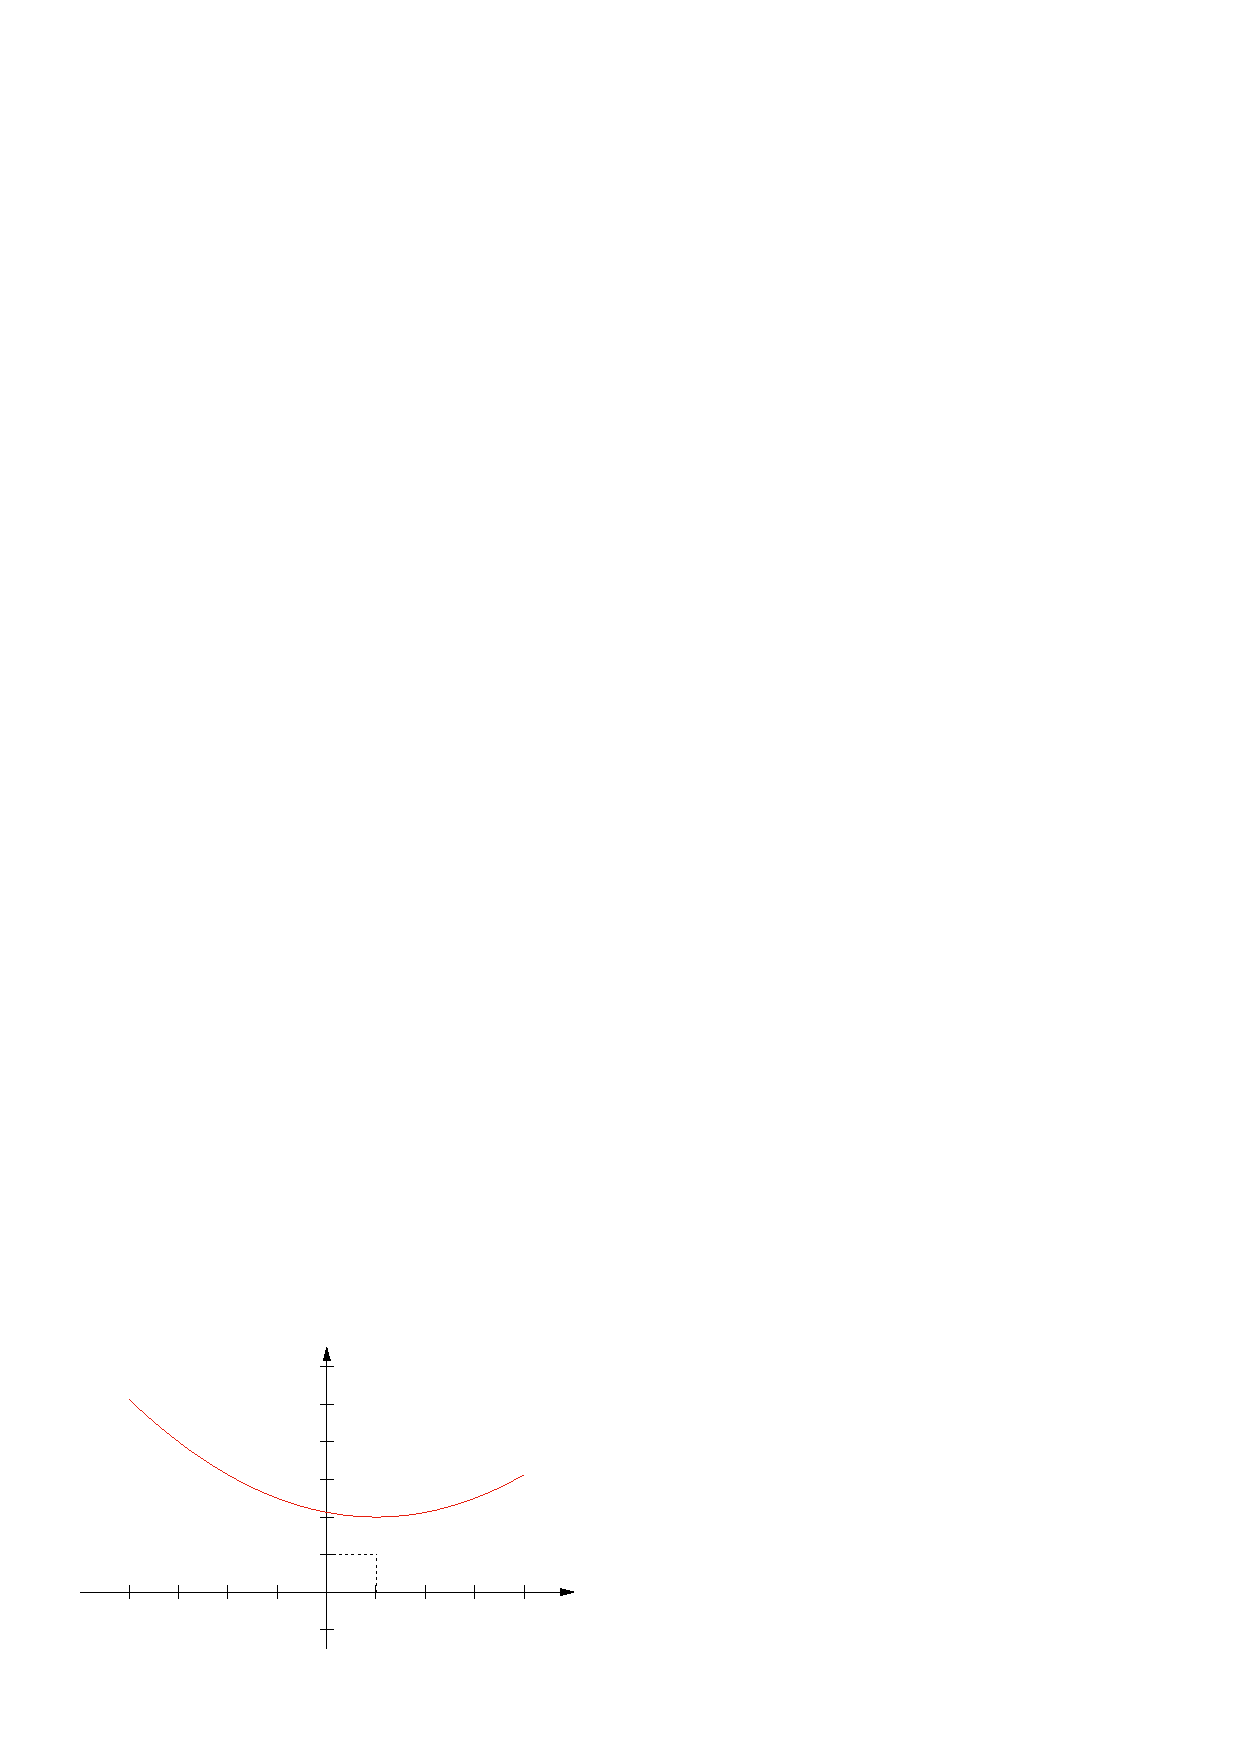
\includegraphics[width={216.00bp},height={144.00bp}]{figura_03_08}}%
    \gplfronttext
  \end{picture}%
\endgroup

\end{figure}
\begin{equation}
    \phi(t)u(t-t_0)=\begin{cases}
        0&t<t_0\\
        \phi(t)&t>t_0\\
    \end{cases}
\end{equation}
\begin{figure}[H]
    \centering
    % GNUPLOT: LaTeX picture with Postscript
\begingroup
  \makeatletter
  \providecommand\color[2][]{%
    \GenericError{(gnuplot) \space\space\space\@spaces}{%
      Package color not loaded in conjunction with
      terminal option `colourtext'%
    }{See the gnuplot documentation for explanation.%
    }{Either use 'blacktext' in gnuplot or load the package
      color.sty in LaTeX.}%
    \renewcommand\color[2][]{}%
  }%
  \providecommand\includegraphics[2][]{%
    \GenericError{(gnuplot) \space\space\space\@spaces}{%
      Package graphicx or graphics not loaded%
    }{See the gnuplot documentation for explanation.%
    }{The gnuplot epslatex terminal needs graphicx.sty or graphics.sty.}%
    \renewcommand\includegraphics[2][]{}%
  }%
  \providecommand\rotatebox[2]{#2}%
  \@ifundefined{ifGPcolor}{%
    \newif\ifGPcolor
    \GPcolorfalse
  }{}%
  \@ifundefined{ifGPblacktext}{%
    \newif\ifGPblacktext
    \GPblacktexttrue
  }{}%
  % define a \g@addto@macro without @ in the name:
  \let\gplgaddtomacro\g@addto@macro
  % define empty templates for all commands taking text:
  \gdef\gplbacktext{}%
  \gdef\gplfronttext{}%
  \makeatother
  \ifGPblacktext
    % no textcolor at all
    \def\colorrgb#1{}%
    \def\colorgray#1{}%
  \else
    % gray or color?
    \ifGPcolor
      \def\colorrgb#1{\color[rgb]{#1}}%
      \def\colorgray#1{\color[gray]{#1}}%
      \expandafter\def\csname LTw\endcsname{\color{white}}%
      \expandafter\def\csname LTb\endcsname{\color{black}}%
      \expandafter\def\csname LTa\endcsname{\color{black}}%
      \expandafter\def\csname LT0\endcsname{\color[rgb]{1,0,0}}%
      \expandafter\def\csname LT1\endcsname{\color[rgb]{0,1,0}}%
      \expandafter\def\csname LT2\endcsname{\color[rgb]{0,0,1}}%
      \expandafter\def\csname LT3\endcsname{\color[rgb]{1,0,1}}%
      \expandafter\def\csname LT4\endcsname{\color[rgb]{0,1,1}}%
      \expandafter\def\csname LT5\endcsname{\color[rgb]{1,1,0}}%
      \expandafter\def\csname LT6\endcsname{\color[rgb]{0,0,0}}%
      \expandafter\def\csname LT7\endcsname{\color[rgb]{1,0.3,0}}%
      \expandafter\def\csname LT8\endcsname{\color[rgb]{0.5,0.5,0.5}}%
    \else
      % gray
      \def\colorrgb#1{\color{black}}%
      \def\colorgray#1{\color[gray]{#1}}%
      \expandafter\def\csname LTw\endcsname{\color{white}}%
      \expandafter\def\csname LTb\endcsname{\color{black}}%
      \expandafter\def\csname LTa\endcsname{\color{black}}%
      \expandafter\def\csname LT0\endcsname{\color{black}}%
      \expandafter\def\csname LT1\endcsname{\color{black}}%
      \expandafter\def\csname LT2\endcsname{\color{black}}%
      \expandafter\def\csname LT3\endcsname{\color{black}}%
      \expandafter\def\csname LT4\endcsname{\color{black}}%
      \expandafter\def\csname LT5\endcsname{\color{black}}%
      \expandafter\def\csname LT6\endcsname{\color{black}}%
      \expandafter\def\csname LT7\endcsname{\color{black}}%
      \expandafter\def\csname LT8\endcsname{\color{black}}%
    \fi
  \fi
    \setlength{\unitlength}{0.0500bp}%
    \ifx\gptboxheight\undefined%
      \newlength{\gptboxheight}%
      \newlength{\gptboxwidth}%
      \newsavebox{\gptboxtext}%
    \fi%
    \setlength{\fboxrule}{0.5pt}%
    \setlength{\fboxsep}{1pt}%
    \definecolor{tbcol}{rgb}{1,1,1}%
\begin{picture}(4320.00,2880.00)%
    \gplgaddtomacro\gplbacktext{%
      \csname LTb\endcsname%%
      \put(2040,192){\makebox(0,0)[r]{\strut{}}}%
      \put(2040,553){\makebox(0,0)[r]{\strut{}}}%
      \put(2040,914){\makebox(0,0)[r]{\strut{}}}%
      \put(2040,1275){\makebox(0,0)[r]{\strut{}}}%
      \put(2040,1636){\makebox(0,0)[r]{\strut{}}}%
      \put(2040,1997){\makebox(0,0)[r]{\strut{}}}%
      \put(2040,2358){\makebox(0,0)[r]{\strut{}}}%
      \put(2040,2719){\makebox(0,0)[r]{\strut{}}}%
      \put(240,330){\makebox(0,0){\strut{}}}%
      \put(714,330){\makebox(0,0){\strut{}}}%
      \put(1188,330){\makebox(0,0){\strut{}}}%
      \put(1662,330){\makebox(0,0){\strut{}}}%
      \put(2136,330){\makebox(0,0){\strut{}}}%
      \put(2609,330){\makebox(0,0){\strut{}}}%
      \put(3083,330){\makebox(0,0){\strut{}}}%
      \put(3557,330){\makebox(0,0){\strut{}}}%
      \put(4031,330){\makebox(0,0){\strut{}}}%
      \csname LTb\endcsname%%
      \put(4647,553){\makebox(0,0)[l]{\strut{}$t$}}%
      \put(2349,2863){\makebox(0,0)[l]{\strut{}$f(t)$}}%
      \put(2562,336){\makebox(0,0)[l]{\strut{}$t_0$}}%
      \put(3083,1095){\makebox(0,0)[l]{\strut{}$\phi(t)u(t-t_0)$}}%
    }%
    \gplgaddtomacro\gplfronttext{%
    }%
    \gplbacktext
    \put(0,0){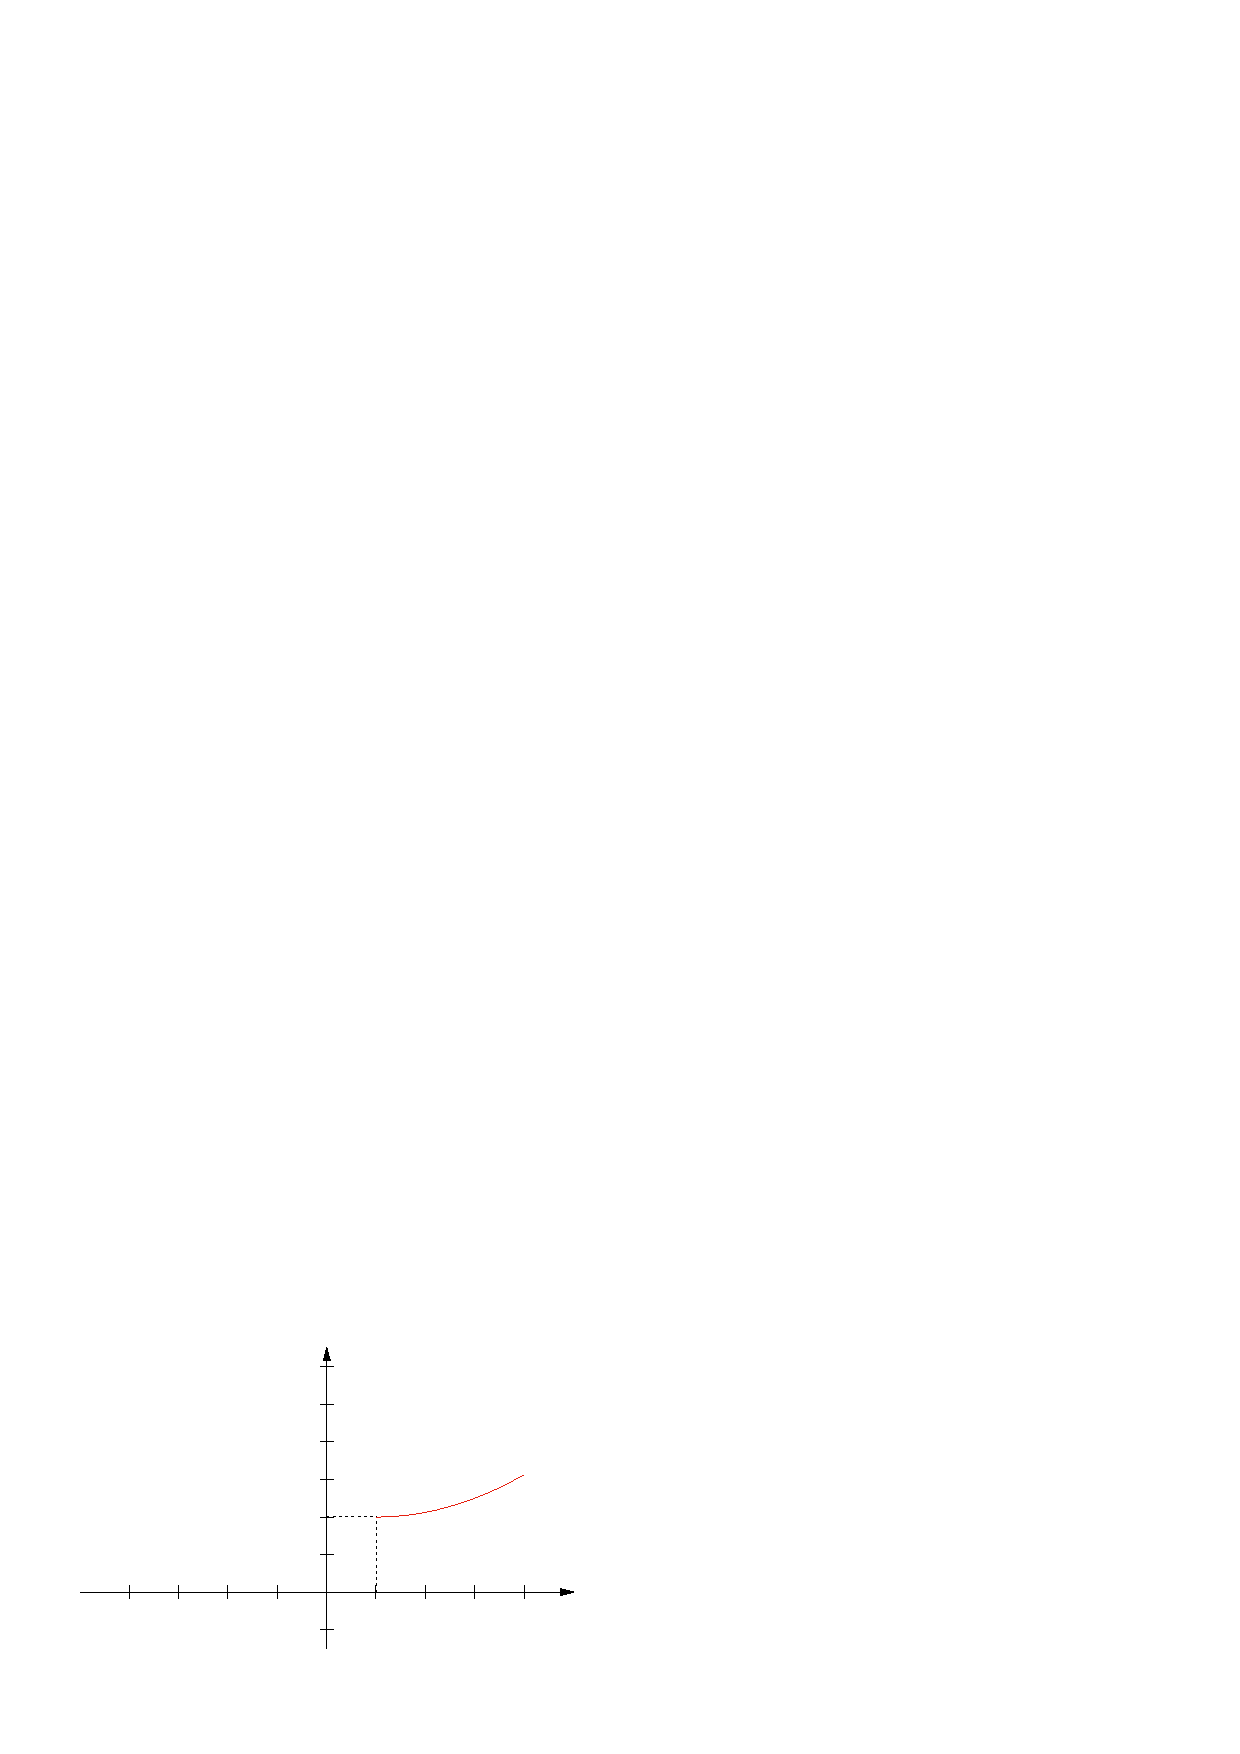
\includegraphics[width={216.00bp},height={144.00bp}]{figura_03_09}}%
    \gplfronttext
  \end{picture}%
\endgroup

\end{figure}
\begin{equation*}
    \phi(t)(u(t-t_1)-u(t-t_2))=\begin{cases}
        0&t\notin[t_1,t_2]\\
        \phi(t)&t\in[t_1,t_2]\\
    \end{cases}
\end{equation*}
\begin{figure}[H]
    \centering
    % GNUPLOT: LaTeX picture with Postscript
\begingroup
  \makeatletter
  \providecommand\color[2][]{%
    \GenericError{(gnuplot) \space\space\space\@spaces}{%
      Package color not loaded in conjunction with
      terminal option `colourtext'%
    }{See the gnuplot documentation for explanation.%
    }{Either use 'blacktext' in gnuplot or load the package
      color.sty in LaTeX.}%
    \renewcommand\color[2][]{}%
  }%
  \providecommand\includegraphics[2][]{%
    \GenericError{(gnuplot) \space\space\space\@spaces}{%
      Package graphicx or graphics not loaded%
    }{See the gnuplot documentation for explanation.%
    }{The gnuplot epslatex terminal needs graphicx.sty or graphics.sty.}%
    \renewcommand\includegraphics[2][]{}%
  }%
  \providecommand\rotatebox[2]{#2}%
  \@ifundefined{ifGPcolor}{%
    \newif\ifGPcolor
    \GPcolorfalse
  }{}%
  \@ifundefined{ifGPblacktext}{%
    \newif\ifGPblacktext
    \GPblacktexttrue
  }{}%
  % define a \g@addto@macro without @ in the name:
  \let\gplgaddtomacro\g@addto@macro
  % define empty templates for all commands taking text:
  \gdef\gplbacktext{}%
  \gdef\gplfronttext{}%
  \makeatother
  \ifGPblacktext
    % no textcolor at all
    \def\colorrgb#1{}%
    \def\colorgray#1{}%
  \else
    % gray or color?
    \ifGPcolor
      \def\colorrgb#1{\color[rgb]{#1}}%
      \def\colorgray#1{\color[gray]{#1}}%
      \expandafter\def\csname LTw\endcsname{\color{white}}%
      \expandafter\def\csname LTb\endcsname{\color{black}}%
      \expandafter\def\csname LTa\endcsname{\color{black}}%
      \expandafter\def\csname LT0\endcsname{\color[rgb]{1,0,0}}%
      \expandafter\def\csname LT1\endcsname{\color[rgb]{0,1,0}}%
      \expandafter\def\csname LT2\endcsname{\color[rgb]{0,0,1}}%
      \expandafter\def\csname LT3\endcsname{\color[rgb]{1,0,1}}%
      \expandafter\def\csname LT4\endcsname{\color[rgb]{0,1,1}}%
      \expandafter\def\csname LT5\endcsname{\color[rgb]{1,1,0}}%
      \expandafter\def\csname LT6\endcsname{\color[rgb]{0,0,0}}%
      \expandafter\def\csname LT7\endcsname{\color[rgb]{1,0.3,0}}%
      \expandafter\def\csname LT8\endcsname{\color[rgb]{0.5,0.5,0.5}}%
    \else
      % gray
      \def\colorrgb#1{\color{black}}%
      \def\colorgray#1{\color[gray]{#1}}%
      \expandafter\def\csname LTw\endcsname{\color{white}}%
      \expandafter\def\csname LTb\endcsname{\color{black}}%
      \expandafter\def\csname LTa\endcsname{\color{black}}%
      \expandafter\def\csname LT0\endcsname{\color{black}}%
      \expandafter\def\csname LT1\endcsname{\color{black}}%
      \expandafter\def\csname LT2\endcsname{\color{black}}%
      \expandafter\def\csname LT3\endcsname{\color{black}}%
      \expandafter\def\csname LT4\endcsname{\color{black}}%
      \expandafter\def\csname LT5\endcsname{\color{black}}%
      \expandafter\def\csname LT6\endcsname{\color{black}}%
      \expandafter\def\csname LT7\endcsname{\color{black}}%
      \expandafter\def\csname LT8\endcsname{\color{black}}%
    \fi
  \fi
    \setlength{\unitlength}{0.0500bp}%
    \ifx\gptboxheight\undefined%
      \newlength{\gptboxheight}%
      \newlength{\gptboxwidth}%
      \newsavebox{\gptboxtext}%
    \fi%
    \setlength{\fboxrule}{0.5pt}%
    \setlength{\fboxsep}{1pt}%
    \definecolor{tbcol}{rgb}{1,1,1}%
\begin{picture}(4320.00,2880.00)%
    \gplgaddtomacro\gplbacktext{%
      \csname LTb\endcsname%%
      \put(2040,192){\makebox(0,0)[r]{\strut{}}}%
      \put(2040,553){\makebox(0,0)[r]{\strut{}}}%
      \put(2040,914){\makebox(0,0)[r]{\strut{}}}%
      \put(2040,1275){\makebox(0,0)[r]{\strut{}}}%
      \put(2040,1636){\makebox(0,0)[r]{\strut{}}}%
      \put(2040,1997){\makebox(0,0)[r]{\strut{}}}%
      \put(2040,2358){\makebox(0,0)[r]{\strut{}}}%
      \put(2040,2719){\makebox(0,0)[r]{\strut{}}}%
      \put(240,330){\makebox(0,0){\strut{}}}%
      \put(714,330){\makebox(0,0){\strut{}}}%
      \put(1188,330){\makebox(0,0){\strut{}}}%
      \put(1662,330){\makebox(0,0){\strut{}}}%
      \put(2136,330){\makebox(0,0){\strut{}}}%
      \put(2609,330){\makebox(0,0){\strut{}}}%
      \put(3083,330){\makebox(0,0){\strut{}}}%
      \put(3557,330){\makebox(0,0){\strut{}}}%
      \put(4031,330){\makebox(0,0){\strut{}}}%
      \csname LTb\endcsname%%
      \put(4647,553){\makebox(0,0)[l]{\strut{}$t$}}%
      \put(2349,2863){\makebox(0,0)[l]{\strut{}$f(t)$}}%
      \put(2562,336){\makebox(0,0)[l]{\strut{}$t_1$}}%
      \put(3510,336){\makebox(0,0)[l]{\strut{}$t_2$}}%
      \put(2609,1817){\makebox(0,0)[l]{\strut{}$\phi(t)(u(t-t_1)-u(t-t_2))$}}%
    }%
    \gplgaddtomacro\gplfronttext{%
    }%
    \gplbacktext
    \put(0,0){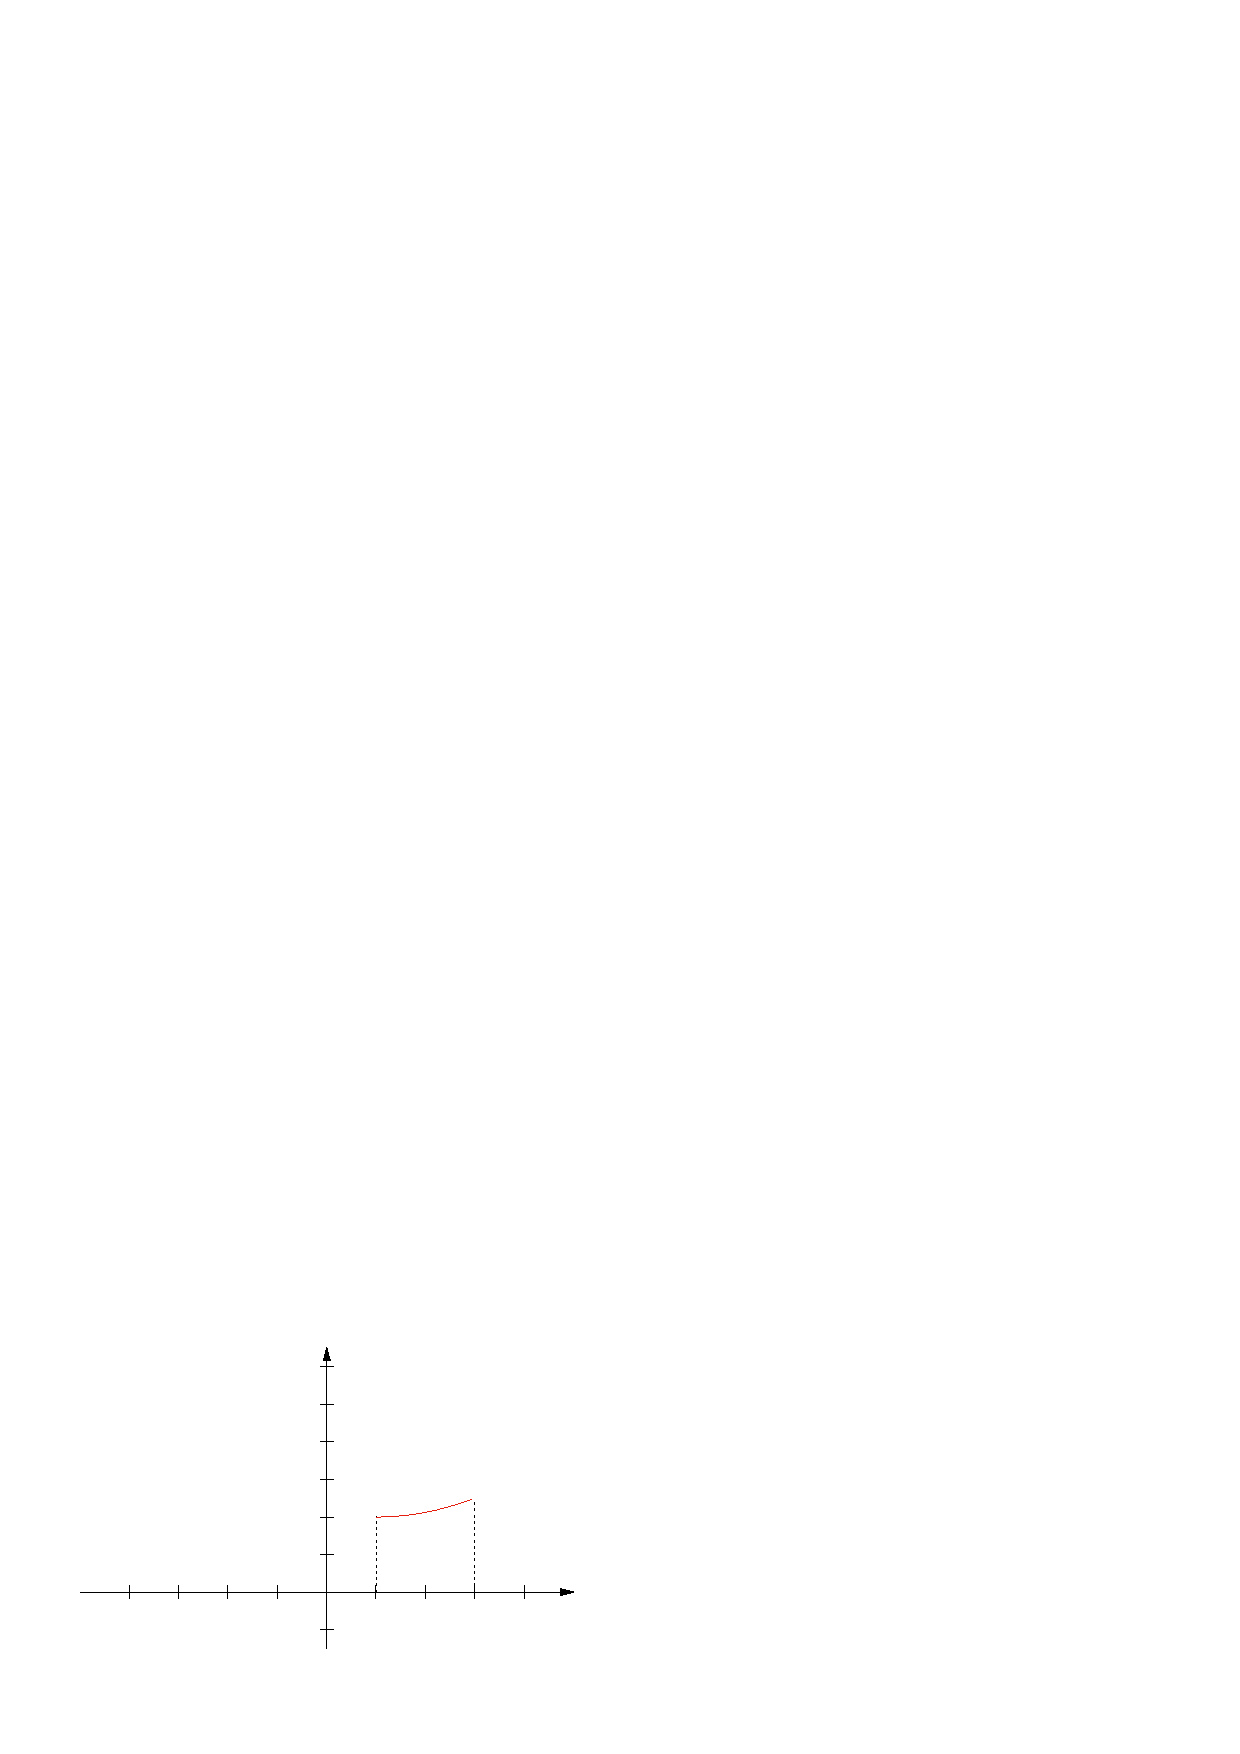
\includegraphics[width={216.00bp},height={144.00bp}]{figura_03_10}}%
    \gplfronttext
  \end{picture}%
\endgroup

\end{figure}

\section{La función impulso}
Pulso rectangular de área igual a 1.
\begin{figure}[H]
    \centering
    % GNUPLOT: LaTeX picture with Postscript
\begingroup
  \makeatletter
  \providecommand\color[2][]{%
    \GenericError{(gnuplot) \space\space\space\@spaces}{%
      Package color not loaded in conjunction with
      terminal option `colourtext'%
    }{See the gnuplot documentation for explanation.%
    }{Either use 'blacktext' in gnuplot or load the package
      color.sty in LaTeX.}%
    \renewcommand\color[2][]{}%
  }%
  \providecommand\includegraphics[2][]{%
    \GenericError{(gnuplot) \space\space\space\@spaces}{%
      Package graphicx or graphics not loaded%
    }{See the gnuplot documentation for explanation.%
    }{The gnuplot epslatex terminal needs graphicx.sty or graphics.sty.}%
    \renewcommand\includegraphics[2][]{}%
  }%
  \providecommand\rotatebox[2]{#2}%
  \@ifundefined{ifGPcolor}{%
    \newif\ifGPcolor
    \GPcolorfalse
  }{}%
  \@ifundefined{ifGPblacktext}{%
    \newif\ifGPblacktext
    \GPblacktexttrue
  }{}%
  % define a \g@addto@macro without @ in the name:
  \let\gplgaddtomacro\g@addto@macro
  % define empty templates for all commands taking text:
  \gdef\gplbacktext{}%
  \gdef\gplfronttext{}%
  \makeatother
  \ifGPblacktext
    % no textcolor at all
    \def\colorrgb#1{}%
    \def\colorgray#1{}%
  \else
    % gray or color?
    \ifGPcolor
      \def\colorrgb#1{\color[rgb]{#1}}%
      \def\colorgray#1{\color[gray]{#1}}%
      \expandafter\def\csname LTw\endcsname{\color{white}}%
      \expandafter\def\csname LTb\endcsname{\color{black}}%
      \expandafter\def\csname LTa\endcsname{\color{black}}%
      \expandafter\def\csname LT0\endcsname{\color[rgb]{1,0,0}}%
      \expandafter\def\csname LT1\endcsname{\color[rgb]{0,1,0}}%
      \expandafter\def\csname LT2\endcsname{\color[rgb]{0,0,1}}%
      \expandafter\def\csname LT3\endcsname{\color[rgb]{1,0,1}}%
      \expandafter\def\csname LT4\endcsname{\color[rgb]{0,1,1}}%
      \expandafter\def\csname LT5\endcsname{\color[rgb]{1,1,0}}%
      \expandafter\def\csname LT6\endcsname{\color[rgb]{0,0,0}}%
      \expandafter\def\csname LT7\endcsname{\color[rgb]{1,0.3,0}}%
      \expandafter\def\csname LT8\endcsname{\color[rgb]{0.5,0.5,0.5}}%
    \else
      % gray
      \def\colorrgb#1{\color{black}}%
      \def\colorgray#1{\color[gray]{#1}}%
      \expandafter\def\csname LTw\endcsname{\color{white}}%
      \expandafter\def\csname LTb\endcsname{\color{black}}%
      \expandafter\def\csname LTa\endcsname{\color{black}}%
      \expandafter\def\csname LT0\endcsname{\color{black}}%
      \expandafter\def\csname LT1\endcsname{\color{black}}%
      \expandafter\def\csname LT2\endcsname{\color{black}}%
      \expandafter\def\csname LT3\endcsname{\color{black}}%
      \expandafter\def\csname LT4\endcsname{\color{black}}%
      \expandafter\def\csname LT5\endcsname{\color{black}}%
      \expandafter\def\csname LT6\endcsname{\color{black}}%
      \expandafter\def\csname LT7\endcsname{\color{black}}%
      \expandafter\def\csname LT8\endcsname{\color{black}}%
    \fi
  \fi
    \setlength{\unitlength}{0.0500bp}%
    \ifx\gptboxheight\undefined%
      \newlength{\gptboxheight}%
      \newlength{\gptboxwidth}%
      \newsavebox{\gptboxtext}%
    \fi%
    \setlength{\fboxrule}{0.5pt}%
    \setlength{\fboxsep}{1pt}%
    \definecolor{tbcol}{rgb}{1,1,1}%
\begin{picture}(2160.00,2160.00)%
    \gplgaddtomacro\gplbacktext{%
      \csname LTb\endcsname%%
      \put(960,192){\makebox(0,0)[r]{\strut{}}}%
      \put(960,644){\makebox(0,0)[r]{\strut{}}}%
      \put(960,1096){\makebox(0,0)[r]{\strut{}}}%
      \put(960,1547){\makebox(0,0)[r]{\strut{}}}%
      \put(960,1999){\makebox(0,0)[r]{\strut{}}}%
      \put(240,421){\makebox(0,0){\strut{}}}%
      \put(648,421){\makebox(0,0){\strut{}}}%
      \put(1056,421){\makebox(0,0){\strut{}}}%
      \put(1463,421){\makebox(0,0){\strut{}}}%
      \put(1871,421){\makebox(0,0){\strut{}}}%
      \csname LTb\endcsname%%
      \put(2279,644){\makebox(0,0)[l]{\strut{}$t$}}%
      \put(1239,2180){\makebox(0,0)[l]{\strut{}$f(t)$}}%
      \put(1422,373){\makebox(0,0)[l]{\strut{}$\xi$}}%
      \put(444,373){\makebox(0,0)[l]{\strut{}$-\xi$}}%
      \put(1626,1547){\makebox(0,0)[l]{\strut{}$\dfrac{1}{2\xi}$}}%
    }%
    \gplgaddtomacro\gplfronttext{%
    }%
    \gplbacktext
    \put(0,0){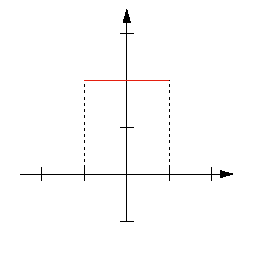
\includegraphics[width={108.00bp},height={108.00bp}]{figura_03_11}}%
    \gplfronttext
  \end{picture}%
\endgroup

\end{figure}

Si $\xi\to0$, entonces $\frac{1}{2\xi}\to\infty$.
\begin{figure}[H]
    \centering
    % GNUPLOT: LaTeX picture with Postscript
\begingroup
  \makeatletter
  \providecommand\color[2][]{%
    \GenericError{(gnuplot) \space\space\space\@spaces}{%
      Package color not loaded in conjunction with
      terminal option `colourtext'%
    }{See the gnuplot documentation for explanation.%
    }{Either use 'blacktext' in gnuplot or load the package
      color.sty in LaTeX.}%
    \renewcommand\color[2][]{}%
  }%
  \providecommand\includegraphics[2][]{%
    \GenericError{(gnuplot) \space\space\space\@spaces}{%
      Package graphicx or graphics not loaded%
    }{See the gnuplot documentation for explanation.%
    }{The gnuplot epslatex terminal needs graphicx.sty or graphics.sty.}%
    \renewcommand\includegraphics[2][]{}%
  }%
  \providecommand\rotatebox[2]{#2}%
  \@ifundefined{ifGPcolor}{%
    \newif\ifGPcolor
    \GPcolorfalse
  }{}%
  \@ifundefined{ifGPblacktext}{%
    \newif\ifGPblacktext
    \GPblacktexttrue
  }{}%
  % define a \g@addto@macro without @ in the name:
  \let\gplgaddtomacro\g@addto@macro
  % define empty templates for all commands taking text:
  \gdef\gplbacktext{}%
  \gdef\gplfronttext{}%
  \makeatother
  \ifGPblacktext
    % no textcolor at all
    \def\colorrgb#1{}%
    \def\colorgray#1{}%
  \else
    % gray or color?
    \ifGPcolor
      \def\colorrgb#1{\color[rgb]{#1}}%
      \def\colorgray#1{\color[gray]{#1}}%
      \expandafter\def\csname LTw\endcsname{\color{white}}%
      \expandafter\def\csname LTb\endcsname{\color{black}}%
      \expandafter\def\csname LTa\endcsname{\color{black}}%
      \expandafter\def\csname LT0\endcsname{\color[rgb]{1,0,0}}%
      \expandafter\def\csname LT1\endcsname{\color[rgb]{0,1,0}}%
      \expandafter\def\csname LT2\endcsname{\color[rgb]{0,0,1}}%
      \expandafter\def\csname LT3\endcsname{\color[rgb]{1,0,1}}%
      \expandafter\def\csname LT4\endcsname{\color[rgb]{0,1,1}}%
      \expandafter\def\csname LT5\endcsname{\color[rgb]{1,1,0}}%
      \expandafter\def\csname LT6\endcsname{\color[rgb]{0,0,0}}%
      \expandafter\def\csname LT7\endcsname{\color[rgb]{1,0.3,0}}%
      \expandafter\def\csname LT8\endcsname{\color[rgb]{0.5,0.5,0.5}}%
    \else
      % gray
      \def\colorrgb#1{\color{black}}%
      \def\colorgray#1{\color[gray]{#1}}%
      \expandafter\def\csname LTw\endcsname{\color{white}}%
      \expandafter\def\csname LTb\endcsname{\color{black}}%
      \expandafter\def\csname LTa\endcsname{\color{black}}%
      \expandafter\def\csname LT0\endcsname{\color{black}}%
      \expandafter\def\csname LT1\endcsname{\color{black}}%
      \expandafter\def\csname LT2\endcsname{\color{black}}%
      \expandafter\def\csname LT3\endcsname{\color{black}}%
      \expandafter\def\csname LT4\endcsname{\color{black}}%
      \expandafter\def\csname LT5\endcsname{\color{black}}%
      \expandafter\def\csname LT6\endcsname{\color{black}}%
      \expandafter\def\csname LT7\endcsname{\color{black}}%
      \expandafter\def\csname LT8\endcsname{\color{black}}%
    \fi
  \fi
    \setlength{\unitlength}{0.0500bp}%
    \ifx\gptboxheight\undefined%
      \newlength{\gptboxheight}%
      \newlength{\gptboxwidth}%
      \newsavebox{\gptboxtext}%
    \fi%
    \setlength{\fboxrule}{0.5pt}%
    \setlength{\fboxsep}{1pt}%
    \definecolor{tbcol}{rgb}{1,1,1}%
\begin{picture}(2160.00,2160.00)%
    \gplgaddtomacro\gplbacktext{%
      \csname LTb\endcsname%%
      \put(960,192){\makebox(0,0)[r]{\strut{}}}%
      \put(960,644){\makebox(0,0)[r]{\strut{}}}%
      \put(960,1096){\makebox(0,0)[r]{\strut{}}}%
      \put(960,1547){\makebox(0,0)[r]{\strut{}}}%
      \put(960,1999){\makebox(0,0)[r]{\strut{}}}%
      \put(240,421){\makebox(0,0){\strut{}}}%
      \put(648,421){\makebox(0,0){\strut{}}}%
      \put(1056,421){\makebox(0,0){\strut{}}}%
      \put(1463,421){\makebox(0,0){\strut{}}}%
      \put(1871,421){\makebox(0,0){\strut{}}}%
      \csname LTb\endcsname%%
      \put(2279,644){\makebox(0,0)[l]{\strut{}$t$}}%
      \put(1239,2180){\makebox(0,0)[l]{\strut{}$f(t)$}}%
      \put(1219,1547){\makebox(0,0)[l]{\strut{}$\delta(t)$}}%
    }%
    \gplgaddtomacro\gplfronttext{%
    }%
    \gplbacktext
    \put(0,0){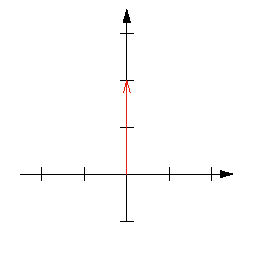
\includegraphics[width={108.00bp},height={108.00bp}]{figura_03_12}}%
    \gplfronttext
  \end{picture}%
\endgroup

\end{figure}
\begin{equation*}
    \delta(t)=\begin{cases}
        0&t\neq0\\
        \infty&t=0\\
    \end{cases}
\end{equation*}

Tal que:
\begin{equation*}
    \int_{-\xi}^{\xi}\delta(t)\,dt=1
\end{equation*}

Por tanto:
\begin{equation}
    k\delta(t)=\begin{cases}
        0&t\neq0\\
        \pm\infty&t=0\\
    \end{cases}
\end{equation}
\begin{figure}[H]
    \centering
    \begin{minipage}{.4\textwidth}
        \centering
        % GNUPLOT: LaTeX picture with Postscript
\begingroup
  \makeatletter
  \providecommand\color[2][]{%
    \GenericError{(gnuplot) \space\space\space\@spaces}{%
      Package color not loaded in conjunction with
      terminal option `colourtext'%
    }{See the gnuplot documentation for explanation.%
    }{Either use 'blacktext' in gnuplot or load the package
      color.sty in LaTeX.}%
    \renewcommand\color[2][]{}%
  }%
  \providecommand\includegraphics[2][]{%
    \GenericError{(gnuplot) \space\space\space\@spaces}{%
      Package graphicx or graphics not loaded%
    }{See the gnuplot documentation for explanation.%
    }{The gnuplot epslatex terminal needs graphicx.sty or graphics.sty.}%
    \renewcommand\includegraphics[2][]{}%
  }%
  \providecommand\rotatebox[2]{#2}%
  \@ifundefined{ifGPcolor}{%
    \newif\ifGPcolor
    \GPcolorfalse
  }{}%
  \@ifundefined{ifGPblacktext}{%
    \newif\ifGPblacktext
    \GPblacktexttrue
  }{}%
  % define a \g@addto@macro without @ in the name:
  \let\gplgaddtomacro\g@addto@macro
  % define empty templates for all commands taking text:
  \gdef\gplbacktext{}%
  \gdef\gplfronttext{}%
  \makeatother
  \ifGPblacktext
    % no textcolor at all
    \def\colorrgb#1{}%
    \def\colorgray#1{}%
  \else
    % gray or color?
    \ifGPcolor
      \def\colorrgb#1{\color[rgb]{#1}}%
      \def\colorgray#1{\color[gray]{#1}}%
      \expandafter\def\csname LTw\endcsname{\color{white}}%
      \expandafter\def\csname LTb\endcsname{\color{black}}%
      \expandafter\def\csname LTa\endcsname{\color{black}}%
      \expandafter\def\csname LT0\endcsname{\color[rgb]{1,0,0}}%
      \expandafter\def\csname LT1\endcsname{\color[rgb]{0,1,0}}%
      \expandafter\def\csname LT2\endcsname{\color[rgb]{0,0,1}}%
      \expandafter\def\csname LT3\endcsname{\color[rgb]{1,0,1}}%
      \expandafter\def\csname LT4\endcsname{\color[rgb]{0,1,1}}%
      \expandafter\def\csname LT5\endcsname{\color[rgb]{1,1,0}}%
      \expandafter\def\csname LT6\endcsname{\color[rgb]{0,0,0}}%
      \expandafter\def\csname LT7\endcsname{\color[rgb]{1,0.3,0}}%
      \expandafter\def\csname LT8\endcsname{\color[rgb]{0.5,0.5,0.5}}%
    \else
      % gray
      \def\colorrgb#1{\color{black}}%
      \def\colorgray#1{\color[gray]{#1}}%
      \expandafter\def\csname LTw\endcsname{\color{white}}%
      \expandafter\def\csname LTb\endcsname{\color{black}}%
      \expandafter\def\csname LTa\endcsname{\color{black}}%
      \expandafter\def\csname LT0\endcsname{\color{black}}%
      \expandafter\def\csname LT1\endcsname{\color{black}}%
      \expandafter\def\csname LT2\endcsname{\color{black}}%
      \expandafter\def\csname LT3\endcsname{\color{black}}%
      \expandafter\def\csname LT4\endcsname{\color{black}}%
      \expandafter\def\csname LT5\endcsname{\color{black}}%
      \expandafter\def\csname LT6\endcsname{\color{black}}%
      \expandafter\def\csname LT7\endcsname{\color{black}}%
      \expandafter\def\csname LT8\endcsname{\color{black}}%
    \fi
  \fi
    \setlength{\unitlength}{0.0500bp}%
    \ifx\gptboxheight\undefined%
      \newlength{\gptboxheight}%
      \newlength{\gptboxwidth}%
      \newsavebox{\gptboxtext}%
    \fi%
    \setlength{\fboxrule}{0.5pt}%
    \setlength{\fboxsep}{1pt}%
    \definecolor{tbcol}{rgb}{1,1,1}%
\begin{picture}(2160.00,2160.00)%
    \gplgaddtomacro\gplbacktext{%
      \csname LTb\endcsname%%
      \put(960,192){\makebox(0,0)[r]{\strut{}}}%
      \put(960,644){\makebox(0,0)[r]{\strut{}}}%
      \put(960,1096){\makebox(0,0)[r]{\strut{}}}%
      \put(960,1547){\makebox(0,0)[r]{\strut{}}}%
      \put(960,1999){\makebox(0,0)[r]{\strut{}}}%
      \put(240,421){\makebox(0,0){\strut{}}}%
      \put(648,421){\makebox(0,0){\strut{}}}%
      \put(1056,421){\makebox(0,0){\strut{}}}%
      \put(1463,421){\makebox(0,0){\strut{}}}%
      \put(1871,421){\makebox(0,0){\strut{}}}%
      \csname LTb\endcsname%%
      \put(2279,644){\makebox(0,0)[l]{\strut{}$t$}}%
      \put(1239,2180){\makebox(0,0)[l]{\strut{}$f(t)$}}%
      \put(1626,1547){\makebox(0,0)[l]{\strut{}$k\delta(t-t_0)$}}%
      \put(1626,1276){\makebox(0,0)[l]{\strut{}$k>0$}}%
      \put(1422,463){\makebox(0,0)[l]{\strut{}$t_0$}}%
    }%
    \gplgaddtomacro\gplfronttext{%
    }%
    \gplbacktext
    \put(0,0){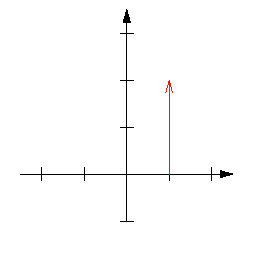
\includegraphics[width={108.00bp},height={108.00bp}]{figura_03_13}}%
    \gplfronttext
  \end{picture}%
\endgroup

    \end{minipage}
    \begin{minipage}{.4\textwidth}
        \centering
        % GNUPLOT: LaTeX picture with Postscript
\begingroup
  \makeatletter
  \providecommand\color[2][]{%
    \GenericError{(gnuplot) \space\space\space\@spaces}{%
      Package color not loaded in conjunction with
      terminal option `colourtext'%
    }{See the gnuplot documentation for explanation.%
    }{Either use 'blacktext' in gnuplot or load the package
      color.sty in LaTeX.}%
    \renewcommand\color[2][]{}%
  }%
  \providecommand\includegraphics[2][]{%
    \GenericError{(gnuplot) \space\space\space\@spaces}{%
      Package graphicx or graphics not loaded%
    }{See the gnuplot documentation for explanation.%
    }{The gnuplot epslatex terminal needs graphicx.sty or graphics.sty.}%
    \renewcommand\includegraphics[2][]{}%
  }%
  \providecommand\rotatebox[2]{#2}%
  \@ifundefined{ifGPcolor}{%
    \newif\ifGPcolor
    \GPcolorfalse
  }{}%
  \@ifundefined{ifGPblacktext}{%
    \newif\ifGPblacktext
    \GPblacktexttrue
  }{}%
  % define a \g@addto@macro without @ in the name:
  \let\gplgaddtomacro\g@addto@macro
  % define empty templates for all commands taking text:
  \gdef\gplbacktext{}%
  \gdef\gplfronttext{}%
  \makeatother
  \ifGPblacktext
    % no textcolor at all
    \def\colorrgb#1{}%
    \def\colorgray#1{}%
  \else
    % gray or color?
    \ifGPcolor
      \def\colorrgb#1{\color[rgb]{#1}}%
      \def\colorgray#1{\color[gray]{#1}}%
      \expandafter\def\csname LTw\endcsname{\color{white}}%
      \expandafter\def\csname LTb\endcsname{\color{black}}%
      \expandafter\def\csname LTa\endcsname{\color{black}}%
      \expandafter\def\csname LT0\endcsname{\color[rgb]{1,0,0}}%
      \expandafter\def\csname LT1\endcsname{\color[rgb]{0,1,0}}%
      \expandafter\def\csname LT2\endcsname{\color[rgb]{0,0,1}}%
      \expandafter\def\csname LT3\endcsname{\color[rgb]{1,0,1}}%
      \expandafter\def\csname LT4\endcsname{\color[rgb]{0,1,1}}%
      \expandafter\def\csname LT5\endcsname{\color[rgb]{1,1,0}}%
      \expandafter\def\csname LT6\endcsname{\color[rgb]{0,0,0}}%
      \expandafter\def\csname LT7\endcsname{\color[rgb]{1,0.3,0}}%
      \expandafter\def\csname LT8\endcsname{\color[rgb]{0.5,0.5,0.5}}%
    \else
      % gray
      \def\colorrgb#1{\color{black}}%
      \def\colorgray#1{\color[gray]{#1}}%
      \expandafter\def\csname LTw\endcsname{\color{white}}%
      \expandafter\def\csname LTb\endcsname{\color{black}}%
      \expandafter\def\csname LTa\endcsname{\color{black}}%
      \expandafter\def\csname LT0\endcsname{\color{black}}%
      \expandafter\def\csname LT1\endcsname{\color{black}}%
      \expandafter\def\csname LT2\endcsname{\color{black}}%
      \expandafter\def\csname LT3\endcsname{\color{black}}%
      \expandafter\def\csname LT4\endcsname{\color{black}}%
      \expandafter\def\csname LT5\endcsname{\color{black}}%
      \expandafter\def\csname LT6\endcsname{\color{black}}%
      \expandafter\def\csname LT7\endcsname{\color{black}}%
      \expandafter\def\csname LT8\endcsname{\color{black}}%
    \fi
  \fi
    \setlength{\unitlength}{0.0500bp}%
    \ifx\gptboxheight\undefined%
      \newlength{\gptboxheight}%
      \newlength{\gptboxwidth}%
      \newsavebox{\gptboxtext}%
    \fi%
    \setlength{\fboxrule}{0.5pt}%
    \setlength{\fboxsep}{1pt}%
    \definecolor{tbcol}{rgb}{1,1,1}%
\begin{picture}(2160.00,2160.00)%
    \gplgaddtomacro\gplbacktext{%
      \csname LTb\endcsname%%
      \put(960,192){\makebox(0,0)[r]{\strut{}}}%
      \put(960,644){\makebox(0,0)[r]{\strut{}}}%
      \put(960,1096){\makebox(0,0)[r]{\strut{}}}%
      \put(960,1547){\makebox(0,0)[r]{\strut{}}}%
      \put(960,1999){\makebox(0,0)[r]{\strut{}}}%
      \put(240,1324){\makebox(0,0){\strut{}}}%
      \put(648,1324){\makebox(0,0){\strut{}}}%
      \put(1056,1324){\makebox(0,0){\strut{}}}%
      \put(1463,1324){\makebox(0,0){\strut{}}}%
      \put(1871,1324){\makebox(0,0){\strut{}}}%
      \csname LTb\endcsname%%
      \put(2279,1547){\makebox(0,0)[l]{\strut{}$t$}}%
      \put(1239,2180){\makebox(0,0)[l]{\strut{}$f(t)$}}%
      \put(1626,644){\makebox(0,0)[l]{\strut{}$k\delta(t-t_0)$}}%
      \put(1626,915){\makebox(0,0)[l]{\strut{}$k<0$}}%
      \put(1422,1728){\makebox(0,0)[l]{\strut{}$t_0$}}%
    }%
    \gplgaddtomacro\gplfronttext{%
    }%
    \gplbacktext
    \put(0,0){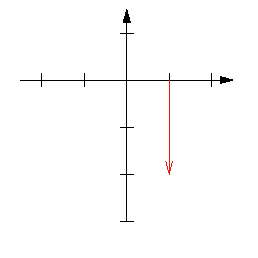
\includegraphics[width={108.00bp},height={108.00bp}]{figura_03_14}}%
    \gplfronttext
  \end{picture}%
\endgroup

    \end{minipage}
\end{figure}

Si: $\phi(t)$ es una función de prueba:
\begin{equation}
    \phi(t)\delta(t-t_0)=\phi(t_0)\delta(t-t_0)
\end{equation}
\begin{figure}[H]
    \centering
    % GNUPLOT: LaTeX picture with Postscript
\begingroup
  \makeatletter
  \providecommand\color[2][]{%
    \GenericError{(gnuplot) \space\space\space\@spaces}{%
      Package color not loaded in conjunction with
      terminal option `colourtext'%
    }{See the gnuplot documentation for explanation.%
    }{Either use 'blacktext' in gnuplot or load the package
      color.sty in LaTeX.}%
    \renewcommand\color[2][]{}%
  }%
  \providecommand\includegraphics[2][]{%
    \GenericError{(gnuplot) \space\space\space\@spaces}{%
      Package graphicx or graphics not loaded%
    }{See the gnuplot documentation for explanation.%
    }{The gnuplot epslatex terminal needs graphicx.sty or graphics.sty.}%
    \renewcommand\includegraphics[2][]{}%
  }%
  \providecommand\rotatebox[2]{#2}%
  \@ifundefined{ifGPcolor}{%
    \newif\ifGPcolor
    \GPcolorfalse
  }{}%
  \@ifundefined{ifGPblacktext}{%
    \newif\ifGPblacktext
    \GPblacktexttrue
  }{}%
  % define a \g@addto@macro without @ in the name:
  \let\gplgaddtomacro\g@addto@macro
  % define empty templates for all commands taking text:
  \gdef\gplbacktext{}%
  \gdef\gplfronttext{}%
  \makeatother
  \ifGPblacktext
    % no textcolor at all
    \def\colorrgb#1{}%
    \def\colorgray#1{}%
  \else
    % gray or color?
    \ifGPcolor
      \def\colorrgb#1{\color[rgb]{#1}}%
      \def\colorgray#1{\color[gray]{#1}}%
      \expandafter\def\csname LTw\endcsname{\color{white}}%
      \expandafter\def\csname LTb\endcsname{\color{black}}%
      \expandafter\def\csname LTa\endcsname{\color{black}}%
      \expandafter\def\csname LT0\endcsname{\color[rgb]{1,0,0}}%
      \expandafter\def\csname LT1\endcsname{\color[rgb]{0,1,0}}%
      \expandafter\def\csname LT2\endcsname{\color[rgb]{0,0,1}}%
      \expandafter\def\csname LT3\endcsname{\color[rgb]{1,0,1}}%
      \expandafter\def\csname LT4\endcsname{\color[rgb]{0,1,1}}%
      \expandafter\def\csname LT5\endcsname{\color[rgb]{1,1,0}}%
      \expandafter\def\csname LT6\endcsname{\color[rgb]{0,0,0}}%
      \expandafter\def\csname LT7\endcsname{\color[rgb]{1,0.3,0}}%
      \expandafter\def\csname LT8\endcsname{\color[rgb]{0.5,0.5,0.5}}%
    \else
      % gray
      \def\colorrgb#1{\color{black}}%
      \def\colorgray#1{\color[gray]{#1}}%
      \expandafter\def\csname LTw\endcsname{\color{white}}%
      \expandafter\def\csname LTb\endcsname{\color{black}}%
      \expandafter\def\csname LTa\endcsname{\color{black}}%
      \expandafter\def\csname LT0\endcsname{\color{black}}%
      \expandafter\def\csname LT1\endcsname{\color{black}}%
      \expandafter\def\csname LT2\endcsname{\color{black}}%
      \expandafter\def\csname LT3\endcsname{\color{black}}%
      \expandafter\def\csname LT4\endcsname{\color{black}}%
      \expandafter\def\csname LT5\endcsname{\color{black}}%
      \expandafter\def\csname LT6\endcsname{\color{black}}%
      \expandafter\def\csname LT7\endcsname{\color{black}}%
      \expandafter\def\csname LT8\endcsname{\color{black}}%
    \fi
  \fi
    \setlength{\unitlength}{0.0500bp}%
    \ifx\gptboxheight\undefined%
      \newlength{\gptboxheight}%
      \newlength{\gptboxwidth}%
      \newsavebox{\gptboxtext}%
    \fi%
    \setlength{\fboxrule}{0.5pt}%
    \setlength{\fboxsep}{1pt}%
    \definecolor{tbcol}{rgb}{1,1,1}%
\begin{picture}(4320.00,2880.00)%
    \gplgaddtomacro\gplbacktext{%
      \csname LTb\endcsname%%
      \put(2040,192){\makebox(0,0)[r]{\strut{}}}%
      \put(2040,553){\makebox(0,0)[r]{\strut{}}}%
      \put(2040,914){\makebox(0,0)[r]{\strut{}}}%
      \put(2040,1275){\makebox(0,0)[r]{\strut{}}}%
      \put(2040,1636){\makebox(0,0)[r]{\strut{}}}%
      \put(2040,1997){\makebox(0,0)[r]{\strut{}}}%
      \put(2040,2358){\makebox(0,0)[r]{\strut{}}}%
      \put(2040,2719){\makebox(0,0)[r]{\strut{}}}%
      \put(240,330){\makebox(0,0){\strut{}}}%
      \put(714,330){\makebox(0,0){\strut{}}}%
      \put(1188,330){\makebox(0,0){\strut{}}}%
      \put(1662,330){\makebox(0,0){\strut{}}}%
      \put(2136,330){\makebox(0,0){\strut{}}}%
      \put(2609,330){\makebox(0,0){\strut{}}}%
      \put(3083,330){\makebox(0,0){\strut{}}}%
      \put(3557,330){\makebox(0,0){\strut{}}}%
      \put(4031,330){\makebox(0,0){\strut{}}}%
      \csname LTb\endcsname%%
      \put(4647,553){\makebox(0,0)[l]{\strut{}$t$}}%
      \put(2349,2863){\makebox(0,0)[l]{\strut{}$f(t)$}}%
      \put(2562,336){\makebox(0,0)[l]{\strut{}$t_0$}}%
      \put(1235,1275){\makebox(0,0)[l]{\strut{}$\phi(t_0)$}}%
      \put(714,2178){\makebox(0,0)[l]{\strut{}$\phi(t)$}}%
      \put(2799,2178){\makebox(0,0)[l]{\strut{}$\delta(t-t_0)$}}%
    }%
    \gplgaddtomacro\gplfronttext{%
    }%
    \gplbacktext
    \put(0,0){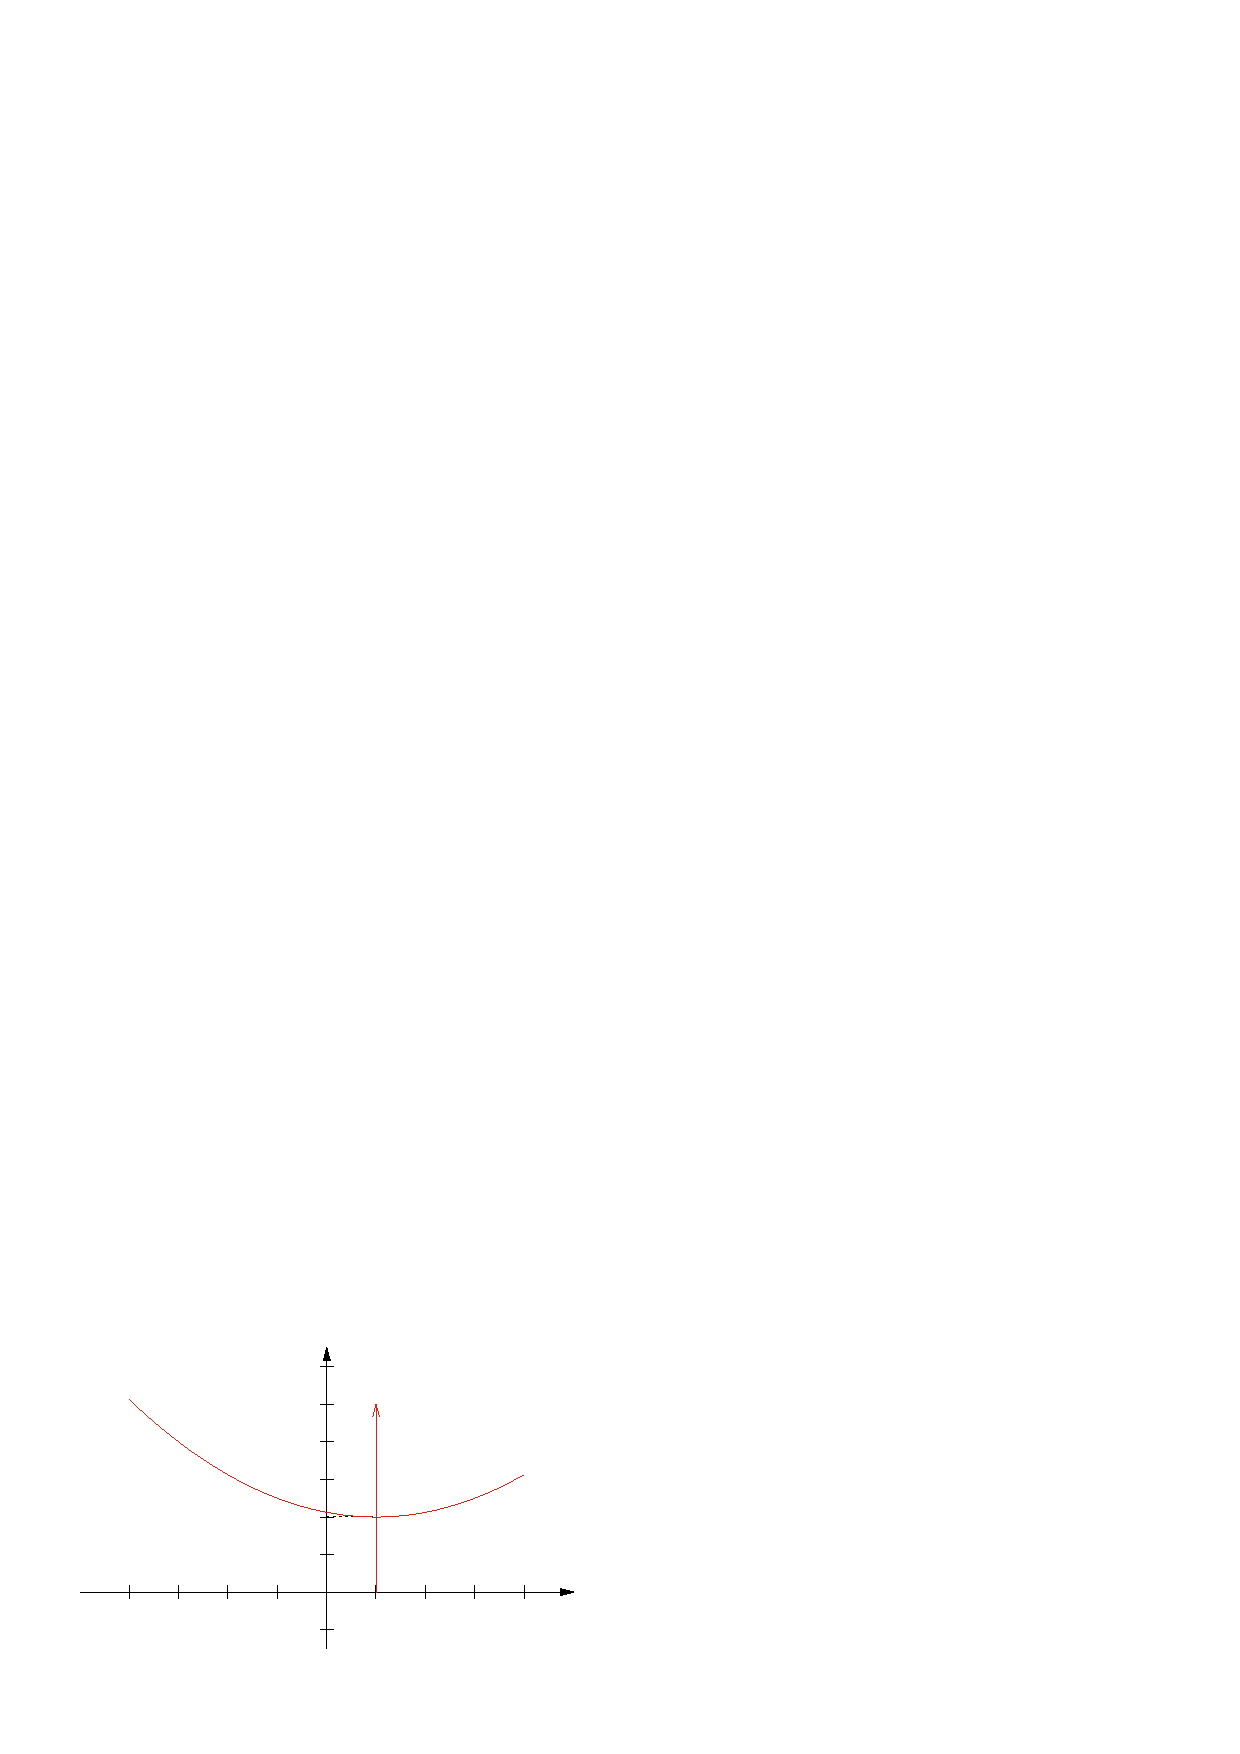
\includegraphics[width={216.00bp},height={144.00bp}]{figura_03_15}}%
    \gplfronttext
  \end{picture}%
\endgroup

\end{figure}

Para $t\neq0$
\begin{equation*}
    \phi(t)\delta(t-t_0)=0
\end{equation*}

Para $t=0$
\begin{equation*}
    \phi(t)\delta(t-t_0)=\phi(t_0)\delta(t-t_0)
\end{equation*}

\subsection{Propiedades de la función impulso}
\subsubsection*{Propiedad 1}
\begin{equation*}
    \int_a^b\delta(t-t_0)\,dt=\begin{cases}
        1&t_0\in[a,b]\\
        0&t_0\notin[a,b]\\
    \end{cases}
\end{equation*}

En general:
\begin{equation}
    \int_{-\infty}^{\infty}\delta(t-t_0)\,dt=1
\end{equation}

\subsubsection*{Propiedad 2}
\begin{equation*}
    \int_a^b\phi(t)\,\delta(t-t_0)\,dt=\begin{cases}
        \phi(t_0)&t_0\in[a,b]\\
        0&t_0\notin[a,b]\\
    \end{cases}
\end{equation*}

En general:
\begin{equation}
    \int_{-\infty}^{\infty}\phi(t_0)\,\delta(t-t_0)\,dt=\phi(t_0)
\end{equation}

\underline{Prueba}:
\begin{equation*}
\begin{split}
    \int_{-\infty}^{\infty}\phi(t)\delta(t-t_0)\,dt
        &=\int_{-\infty}^{\infty}\phi(t_0)\delta(t-t_0)\,dt\\
        &=\phi(t_0)\int_{-\infty}^{\infty}\delta(t-t_0)\,dt\\
        &=\phi(t_0)\\
\end{split}
\end{equation*}

\subsubsection*{Propiedad 3}
\begin{equation}
    \int_{-\infty}^{\infty}\phi(t)\,\delta(at)\,dt
        =\frac{1}{|a|}\int_{-\infty}^{\infty}
            \phi\left(\frac{t}{a}\right)\delta(t)\,dt
        =\frac{\phi(0)}{|a|};a\neq0
\end{equation}

\underline{Prueba}:

Realizando un cambio de variable:
\begin{equation*}
    \tau=at
\end{equation*}
\begin{equation*}
    d\tau=a\,dt
\end{equation*}

Para $a>0$:
\begin{equation*}
    \int_{-\infty}^{\infty}
        \phi\left(\frac{\tau}{a}\right)\delta(\tau)\,\frac{d\tau}{a}
        =\frac{1}{a}\int_{-\infty}^{\infty}
            \phi\left(\frac{\tau}{a}\right)\delta(\tau)d\tau
\end{equation*}

Para $a<0$:
\begin{equation*}
    \int_{-\infty}^{\infty}
        \phi\left(\frac{\tau}{a}\right)\delta(\tau)\,\frac{d\tau}{a}
        =-\frac{1}{a}\int_{-\infty}^{\infty}
            \phi\left(\frac{\tau}{a}\right)\delta(\tau)d\tau
\end{equation*}

Como:
\begin{equation*}
    |a|=\begin{cases}
        -a&a<0\\
        a&a>0\\
    \end{cases}
\end{equation*}
\begin{equation*}
\begin{split}
    \int_{-\infty}^{\infty}\phi(t)\,\delta(at)\,dt
        &=\frac{1}{|a|}\int_{-\infty}^{\infty}
            \phi\left(\frac{\tau}{a}\right)\delta(\tau)\,d\tau\\
        &=\frac{1}{|a|}\phi\left(\frac{0}{a}\right)\\
        &=\frac{\phi(0)}{|a|}\\
\end{split}
\end{equation*}

\subsubsection*{Propiedad 4}
\begin{equation}
    \delta(at)=\frac{1}{|a|}\delta(t)
\end{equation}

En particular:
\begin{equation}
    \delta(-t)=\delta(t)
\end{equation}

Por tanto $\delta(t)$ es una función \textbf{par}.

\underline{Prueba}:
\begin{equation*}
\begin{split}
    \int_{-\infty}^{\infty}\phi(t)\,\delta(at)\,dt
        &=\frac{1}{|a|}\phi(0)\\
        &=\frac{1}{|a|}\int_{-\infty}^{\infty}\phi(t)\,\delta(t)\,dt\\
\end{split}
\end{equation*}
\begin{equation*}
    \phi(t)\,\delta(at)=\frac{1}{|a|}\phi(t)\,\delta(t)
\end{equation*}
\begin{equation*}
    \delta(at)=\frac{1}{|a|}\,\delta(t)
\end{equation*}

Para $a=-1$:
\begin{equation*}
    \delta(-t)=\frac{1}{|-1|}\,\delta(t)=\delta(t)
\end{equation*}

\subsubsection*{Propiedad 5}
\begin{equation*}
    t\,\delta(t)=0
\end{equation*}
\begin{equation}
    t^n\,\delta(t)=0;n\in\mathbb{N}
\end{equation}

\underline{Prueba}:

\begin{equation*}
    \int_{-\infty}^{\infty}t^n\,\delta(t)\,dt=0^n=0
\end{equation*}

Derivando ambos miembros:
\begin{equation*}
    t^n\,\delta(t)\,dt=0
\end{equation*}

\section{Derivada de la función impulso}
\begin{equation*}
    \delta'(t)=\frac{d}{dt}(\delta(t))
\end{equation*}
\begin{equation}
    \int_{-\infty}^{\infty}\phi(t)\delta'(t)\,dt
        =-\int_{-\infty}^{\infty}\phi'(t)\delta(t)\,dt
        =-\phi'(0)
\end{equation}

\underline{Prueba}:

Realizando la integración por partes:
\begin{equation*}
    u=\phi(t)
\end{equation*}
\begin{equation*}
    du=\phi'(t)\,dt
\end{equation*}
\begin{equation*}
    dv=\delta'(t-t_0)\,dt
\end{equation*}
\begin{equation*}
    v=\delta(t-t_0)
\end{equation*}
\begin{equation*}
\begin{split}
    \int_{-\infty}^{\infty}\phi(t)\delta'(t-t_0)\,dt
        &=(\phi(t)\delta(t-t_0)\Big|_{-\infty}^{\infty})
        -\int_{-\infty}^{\infty}\delta(t-t_0)\phi'(t)\,dt\\
        &=0-\int_{-\infty}^{\infty}\delta(t-t_0)\phi'(t)\,dt\\
        &=-\phi'(t_0)
\end{split}
\end{equation*}

\subsubsection{Derivadas de orden superior}
\begin{equation*}
\begin{split}
    \int_{-\infty}^{\infty}\phi(t)\delta''(t)\,dt
        &=\int_{-\infty}^{\infty}\phi(t)(\delta'(t))'\,dt\\
        &=-\int_{-\infty}^{\infty}\phi'(t)\delta'(t)\,dt\\
        &=\int_{-\infty}^{\infty}\phi''(t)\delta(t)\,dt\\
        &=\phi''(0)\\
\end{split}
\end{equation*}

De igual manera:
\begin{equation*}
    \int_{-\infty}^{\infty}\phi(t)\delta^{\prime\prime\prime}(t-t_0)\,dt
        =-\phi^{\prime\prime\prime}(t_0)
\end{equation*}

En general:
\begin{equation}
    \int_{-\infty}^{\infty}\phi(t)\delta^{(n)}(t-t_0)\,dt
        ={(-1)}^n\phi^{(n)}(t_0)
\end{equation}

\section{Derivada de la función escalón unitario}
\begin{figure}[H]
    \centering
    \begin{minipage}{.4\textwidth}
        \centering
        % GNUPLOT: LaTeX picture with Postscript
\begingroup
  \makeatletter
  \providecommand\color[2][]{%
    \GenericError{(gnuplot) \space\space\space\@spaces}{%
      Package color not loaded in conjunction with
      terminal option `colourtext'%
    }{See the gnuplot documentation for explanation.%
    }{Either use 'blacktext' in gnuplot or load the package
      color.sty in LaTeX.}%
    \renewcommand\color[2][]{}%
  }%
  \providecommand\includegraphics[2][]{%
    \GenericError{(gnuplot) \space\space\space\@spaces}{%
      Package graphicx or graphics not loaded%
    }{See the gnuplot documentation for explanation.%
    }{The gnuplot epslatex terminal needs graphicx.sty or graphics.sty.}%
    \renewcommand\includegraphics[2][]{}%
  }%
  \providecommand\rotatebox[2]{#2}%
  \@ifundefined{ifGPcolor}{%
    \newif\ifGPcolor
    \GPcolorfalse
  }{}%
  \@ifundefined{ifGPblacktext}{%
    \newif\ifGPblacktext
    \GPblacktexttrue
  }{}%
  % define a \g@addto@macro without @ in the name:
  \let\gplgaddtomacro\g@addto@macro
  % define empty templates for all commands taking text:
  \gdef\gplbacktext{}%
  \gdef\gplfronttext{}%
  \makeatother
  \ifGPblacktext
    % no textcolor at all
    \def\colorrgb#1{}%
    \def\colorgray#1{}%
  \else
    % gray or color?
    \ifGPcolor
      \def\colorrgb#1{\color[rgb]{#1}}%
      \def\colorgray#1{\color[gray]{#1}}%
      \expandafter\def\csname LTw\endcsname{\color{white}}%
      \expandafter\def\csname LTb\endcsname{\color{black}}%
      \expandafter\def\csname LTa\endcsname{\color{black}}%
      \expandafter\def\csname LT0\endcsname{\color[rgb]{1,0,0}}%
      \expandafter\def\csname LT1\endcsname{\color[rgb]{0,1,0}}%
      \expandafter\def\csname LT2\endcsname{\color[rgb]{0,0,1}}%
      \expandafter\def\csname LT3\endcsname{\color[rgb]{1,0,1}}%
      \expandafter\def\csname LT4\endcsname{\color[rgb]{0,1,1}}%
      \expandafter\def\csname LT5\endcsname{\color[rgb]{1,1,0}}%
      \expandafter\def\csname LT6\endcsname{\color[rgb]{0,0,0}}%
      \expandafter\def\csname LT7\endcsname{\color[rgb]{1,0.3,0}}%
      \expandafter\def\csname LT8\endcsname{\color[rgb]{0.5,0.5,0.5}}%
    \else
      % gray
      \def\colorrgb#1{\color{black}}%
      \def\colorgray#1{\color[gray]{#1}}%
      \expandafter\def\csname LTw\endcsname{\color{white}}%
      \expandafter\def\csname LTb\endcsname{\color{black}}%
      \expandafter\def\csname LTa\endcsname{\color{black}}%
      \expandafter\def\csname LT0\endcsname{\color{black}}%
      \expandafter\def\csname LT1\endcsname{\color{black}}%
      \expandafter\def\csname LT2\endcsname{\color{black}}%
      \expandafter\def\csname LT3\endcsname{\color{black}}%
      \expandafter\def\csname LT4\endcsname{\color{black}}%
      \expandafter\def\csname LT5\endcsname{\color{black}}%
      \expandafter\def\csname LT6\endcsname{\color{black}}%
      \expandafter\def\csname LT7\endcsname{\color{black}}%
      \expandafter\def\csname LT8\endcsname{\color{black}}%
    \fi
  \fi
    \setlength{\unitlength}{0.0500bp}%
    \ifx\gptboxheight\undefined%
      \newlength{\gptboxheight}%
      \newlength{\gptboxwidth}%
      \newsavebox{\gptboxtext}%
    \fi%
    \setlength{\fboxrule}{0.5pt}%
    \setlength{\fboxsep}{1pt}%
    \definecolor{tbcol}{rgb}{1,1,1}%
\begin{picture}(3600.00,2160.00)%
    \gplgaddtomacro\gplbacktext{%
      \csname LTb\endcsname%%
      \put(1680,192){\makebox(0,0)[r]{\strut{}}}%
      \put(1680,553){\makebox(0,0)[r]{\strut{}}}%
      \put(1680,915){\makebox(0,0)[r]{\strut{}}}%
      \put(1680,1276){\makebox(0,0)[r]{\strut{}}}%
      \put(1680,1638){\makebox(0,0)[r]{\strut{}}}%
      \put(1680,1999){\makebox(0,0)[r]{\strut{}}}%
      \put(240,330){\makebox(0,0){\strut{}}}%
      \put(624,330){\makebox(0,0){\strut{}}}%
      \put(1008,330){\makebox(0,0){\strut{}}}%
      \put(1392,330){\makebox(0,0){\strut{}}}%
      \put(1776,330){\makebox(0,0){\strut{}}}%
      \put(2159,330){\makebox(0,0){\strut{}}}%
      \put(2543,330){\makebox(0,0){\strut{}}}%
      \put(2927,330){\makebox(0,0){\strut{}}}%
      \put(3311,330){\makebox(0,0){\strut{}}}%
      \csname LTb\endcsname%%
      \put(3580,553){\makebox(0,0)[l]{\strut{}$t$}}%
      \put(1219,2107){\makebox(0,0)[l]{\strut{}$f(t)$}}%
      \put(1488,915){\makebox(0,0)[l]{\strut{}$1$}}%
      \put(2121,337){\makebox(0,0)[l]{\strut{}$t_0$}}%
      \put(2313,1059){\makebox(0,0)[l]{\strut{}$u(t-t_0)$}}%
    }%
    \gplgaddtomacro\gplfronttext{%
    }%
    \gplbacktext
    \put(0,0){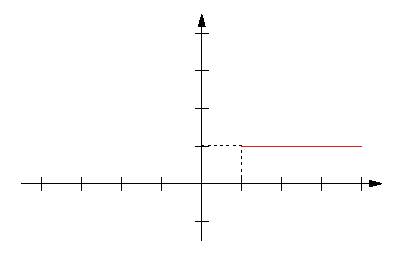
\includegraphics[width={180.00bp},height={108.00bp}]{figura_03_16}}%
    \gplfronttext
  \end{picture}%
\endgroup

    \end{minipage}
    \begin{minipage}{.4\textwidth}
        \centering
        % GNUPLOT: LaTeX picture with Postscript
\begingroup
  \makeatletter
  \providecommand\color[2][]{%
    \GenericError{(gnuplot) \space\space\space\@spaces}{%
      Package color not loaded in conjunction with
      terminal option `colourtext'%
    }{See the gnuplot documentation for explanation.%
    }{Either use 'blacktext' in gnuplot or load the package
      color.sty in LaTeX.}%
    \renewcommand\color[2][]{}%
  }%
  \providecommand\includegraphics[2][]{%
    \GenericError{(gnuplot) \space\space\space\@spaces}{%
      Package graphicx or graphics not loaded%
    }{See the gnuplot documentation for explanation.%
    }{The gnuplot epslatex terminal needs graphicx.sty or graphics.sty.}%
    \renewcommand\includegraphics[2][]{}%
  }%
  \providecommand\rotatebox[2]{#2}%
  \@ifundefined{ifGPcolor}{%
    \newif\ifGPcolor
    \GPcolorfalse
  }{}%
  \@ifundefined{ifGPblacktext}{%
    \newif\ifGPblacktext
    \GPblacktexttrue
  }{}%
  % define a \g@addto@macro without @ in the name:
  \let\gplgaddtomacro\g@addto@macro
  % define empty templates for all commands taking text:
  \gdef\gplbacktext{}%
  \gdef\gplfronttext{}%
  \makeatother
  \ifGPblacktext
    % no textcolor at all
    \def\colorrgb#1{}%
    \def\colorgray#1{}%
  \else
    % gray or color?
    \ifGPcolor
      \def\colorrgb#1{\color[rgb]{#1}}%
      \def\colorgray#1{\color[gray]{#1}}%
      \expandafter\def\csname LTw\endcsname{\color{white}}%
      \expandafter\def\csname LTb\endcsname{\color{black}}%
      \expandafter\def\csname LTa\endcsname{\color{black}}%
      \expandafter\def\csname LT0\endcsname{\color[rgb]{1,0,0}}%
      \expandafter\def\csname LT1\endcsname{\color[rgb]{0,1,0}}%
      \expandafter\def\csname LT2\endcsname{\color[rgb]{0,0,1}}%
      \expandafter\def\csname LT3\endcsname{\color[rgb]{1,0,1}}%
      \expandafter\def\csname LT4\endcsname{\color[rgb]{0,1,1}}%
      \expandafter\def\csname LT5\endcsname{\color[rgb]{1,1,0}}%
      \expandafter\def\csname LT6\endcsname{\color[rgb]{0,0,0}}%
      \expandafter\def\csname LT7\endcsname{\color[rgb]{1,0.3,0}}%
      \expandafter\def\csname LT8\endcsname{\color[rgb]{0.5,0.5,0.5}}%
    \else
      % gray
      \def\colorrgb#1{\color{black}}%
      \def\colorgray#1{\color[gray]{#1}}%
      \expandafter\def\csname LTw\endcsname{\color{white}}%
      \expandafter\def\csname LTb\endcsname{\color{black}}%
      \expandafter\def\csname LTa\endcsname{\color{black}}%
      \expandafter\def\csname LT0\endcsname{\color{black}}%
      \expandafter\def\csname LT1\endcsname{\color{black}}%
      \expandafter\def\csname LT2\endcsname{\color{black}}%
      \expandafter\def\csname LT3\endcsname{\color{black}}%
      \expandafter\def\csname LT4\endcsname{\color{black}}%
      \expandafter\def\csname LT5\endcsname{\color{black}}%
      \expandafter\def\csname LT6\endcsname{\color{black}}%
      \expandafter\def\csname LT7\endcsname{\color{black}}%
      \expandafter\def\csname LT8\endcsname{\color{black}}%
    \fi
  \fi
    \setlength{\unitlength}{0.0500bp}%
    \ifx\gptboxheight\undefined%
      \newlength{\gptboxheight}%
      \newlength{\gptboxwidth}%
      \newsavebox{\gptboxtext}%
    \fi%
    \setlength{\fboxrule}{0.5pt}%
    \setlength{\fboxsep}{1pt}%
    \definecolor{tbcol}{rgb}{1,1,1}%
\begin{picture}(3600.00,2160.00)%
    \gplgaddtomacro\gplbacktext{%
      \csname LTb\endcsname%%
      \put(1680,192){\makebox(0,0)[r]{\strut{}}}%
      \put(1680,553){\makebox(0,0)[r]{\strut{}}}%
      \put(1680,915){\makebox(0,0)[r]{\strut{}}}%
      \put(1680,1276){\makebox(0,0)[r]{\strut{}}}%
      \put(1680,1638){\makebox(0,0)[r]{\strut{}}}%
      \put(1680,1999){\makebox(0,0)[r]{\strut{}}}%
      \put(240,330){\makebox(0,0){\strut{}}}%
      \put(624,330){\makebox(0,0){\strut{}}}%
      \put(1008,330){\makebox(0,0){\strut{}}}%
      \put(1392,330){\makebox(0,0){\strut{}}}%
      \put(1776,330){\makebox(0,0){\strut{}}}%
      \put(2159,330){\makebox(0,0){\strut{}}}%
      \put(2543,330){\makebox(0,0){\strut{}}}%
      \put(2927,330){\makebox(0,0){\strut{}}}%
      \put(3311,330){\makebox(0,0){\strut{}}}%
      \csname LTb\endcsname%%
      \put(3580,553){\makebox(0,0)[l]{\strut{}$t$}}%
      \put(1219,2107){\makebox(0,0)[l]{\strut{}$f^\prime(t)$}}%
      \put(2121,337){\makebox(0,0)[l]{\strut{}$t_0$}}%
      \put(2313,1276){\makebox(0,0)[l]{\strut{}$\delta(t-t_0)$}}%
    }%
    \gplgaddtomacro\gplfronttext{%
    }%
    \gplbacktext
    \put(0,0){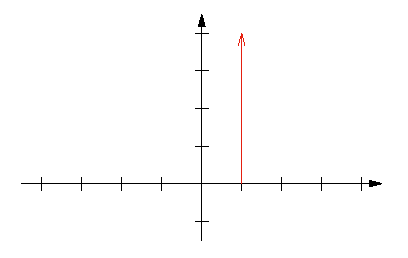
\includegraphics[width={180.00bp},height={108.00bp}]{figura_03_17}}%
    \gplfronttext
  \end{picture}%
\endgroup

    \end{minipage}
\end{figure}
\begin{equation}
    u'(t-t_0)=\delta(t-t_0)
\end{equation}

\underline{Prueba}:

\begin{equation*}
    \int_{-\infty}^{\infty}u'(t)\phi(t)\,dt
\end{equation*}

Realizando la integración por partes:
\begin{equation*}
    u=\phi(t)
\end{equation*}
\begin{equation*}
    du=\phi'(t)\,dt
\end{equation*}
\begin{equation*}
    dv=u'(t)\,dt
\end{equation*}
\begin{equation*}
    v=u(t)
\end{equation*}
\begin{equation*}
\begin{split}
    \int_{-\infty}^{\infty}\phi(t)u'(t)\,dt
        &=(\phi(t)u(t)\Big|_{-\infty}^{\infty})
        -\int_{-\infty}^{\infty}u(t)\phi'(t)\,dt\\
        &=-\int_{-\infty}^{\infty}u(t)\phi'(t)\,dt\\
        &=-\int_{0}^{\infty}1\,\phi'(t)\,dt\\
        &=-\phi(t)\Big|_0^{\infty}\\
        &=-\phi(\infty)+\phi(0)\\
\end{split}
\end{equation*}

Asumiendo que $\phi(\pm\infty)=0$:
\begin{equation*}
    \int_{-\infty}^{\infty}\phi(t)u'(t)\,dt=\phi(0)
\end{equation*}

Sabiendo que:
\begin{equation*}
    \int_{-\infty}^{\infty}\phi(t)\delta(t)\,dt=\phi(0)
\end{equation*}

Por tanto:
\begin{equation*}
    \int_{-\infty}^{\infty}\phi(t)u'(t)\,dt
        =\int_{-\infty}^{\infty}\phi(t)\delta(t)\,dt
\end{equation*}
\begin{equation*}
    \phi(t)u'(t)=\phi(t)\delta(t)
\end{equation*}
\begin{equation*}
    u'(t)=\delta(t)
\end{equation*}

\section{Derivada de una función con discontinuidades de salto}
Las derivadas de los saltos de subida y bajada, van a originar impulsos hacia
arriba y hacia abajo, respectivamente.
\begin{figure}[H]
    \centering
    \begin{minipage}{.4\textwidth}
        \centering
        % GNUPLOT: LaTeX picture with Postscript
\begingroup
  \makeatletter
  \providecommand\color[2][]{%
    \GenericError{(gnuplot) \space\space\space\@spaces}{%
      Package color not loaded in conjunction with
      terminal option `colourtext'%
    }{See the gnuplot documentation for explanation.%
    }{Either use 'blacktext' in gnuplot or load the package
      color.sty in LaTeX.}%
    \renewcommand\color[2][]{}%
  }%
  \providecommand\includegraphics[2][]{%
    \GenericError{(gnuplot) \space\space\space\@spaces}{%
      Package graphicx or graphics not loaded%
    }{See the gnuplot documentation for explanation.%
    }{The gnuplot epslatex terminal needs graphicx.sty or graphics.sty.}%
    \renewcommand\includegraphics[2][]{}%
  }%
  \providecommand\rotatebox[2]{#2}%
  \@ifundefined{ifGPcolor}{%
    \newif\ifGPcolor
    \GPcolorfalse
  }{}%
  \@ifundefined{ifGPblacktext}{%
    \newif\ifGPblacktext
    \GPblacktexttrue
  }{}%
  % define a \g@addto@macro without @ in the name:
  \let\gplgaddtomacro\g@addto@macro
  % define empty templates for all commands taking text:
  \gdef\gplbacktext{}%
  \gdef\gplfronttext{}%
  \makeatother
  \ifGPblacktext
    % no textcolor at all
    \def\colorrgb#1{}%
    \def\colorgray#1{}%
  \else
    % gray or color?
    \ifGPcolor
      \def\colorrgb#1{\color[rgb]{#1}}%
      \def\colorgray#1{\color[gray]{#1}}%
      \expandafter\def\csname LTw\endcsname{\color{white}}%
      \expandafter\def\csname LTb\endcsname{\color{black}}%
      \expandafter\def\csname LTa\endcsname{\color{black}}%
      \expandafter\def\csname LT0\endcsname{\color[rgb]{1,0,0}}%
      \expandafter\def\csname LT1\endcsname{\color[rgb]{0,1,0}}%
      \expandafter\def\csname LT2\endcsname{\color[rgb]{0,0,1}}%
      \expandafter\def\csname LT3\endcsname{\color[rgb]{1,0,1}}%
      \expandafter\def\csname LT4\endcsname{\color[rgb]{0,1,1}}%
      \expandafter\def\csname LT5\endcsname{\color[rgb]{1,1,0}}%
      \expandafter\def\csname LT6\endcsname{\color[rgb]{0,0,0}}%
      \expandafter\def\csname LT7\endcsname{\color[rgb]{1,0.3,0}}%
      \expandafter\def\csname LT8\endcsname{\color[rgb]{0.5,0.5,0.5}}%
    \else
      % gray
      \def\colorrgb#1{\color{black}}%
      \def\colorgray#1{\color[gray]{#1}}%
      \expandafter\def\csname LTw\endcsname{\color{white}}%
      \expandafter\def\csname LTb\endcsname{\color{black}}%
      \expandafter\def\csname LTa\endcsname{\color{black}}%
      \expandafter\def\csname LT0\endcsname{\color{black}}%
      \expandafter\def\csname LT1\endcsname{\color{black}}%
      \expandafter\def\csname LT2\endcsname{\color{black}}%
      \expandafter\def\csname LT3\endcsname{\color{black}}%
      \expandafter\def\csname LT4\endcsname{\color{black}}%
      \expandafter\def\csname LT5\endcsname{\color{black}}%
      \expandafter\def\csname LT6\endcsname{\color{black}}%
      \expandafter\def\csname LT7\endcsname{\color{black}}%
      \expandafter\def\csname LT8\endcsname{\color{black}}%
    \fi
  \fi
    \setlength{\unitlength}{0.0500bp}%
    \ifx\gptboxheight\undefined%
      \newlength{\gptboxheight}%
      \newlength{\gptboxwidth}%
      \newsavebox{\gptboxtext}%
    \fi%
    \setlength{\fboxrule}{0.5pt}%
    \setlength{\fboxsep}{1pt}%
    \definecolor{tbcol}{rgb}{1,1,1}%
\begin{picture}(3600.00,2160.00)%
    \gplgaddtomacro\gplbacktext{%
      \csname LTb\endcsname%%
      \put(1680,192){\makebox(0,0)[r]{\strut{}}}%
      \put(1680,553){\makebox(0,0)[r]{\strut{}}}%
      \put(1680,915){\makebox(0,0)[r]{\strut{}}}%
      \put(1680,1276){\makebox(0,0)[r]{\strut{}}}%
      \put(1680,1638){\makebox(0,0)[r]{\strut{}}}%
      \put(1680,1999){\makebox(0,0)[r]{\strut{}}}%
      \put(240,330){\makebox(0,0){\strut{}}}%
      \put(624,330){\makebox(0,0){\strut{}}}%
      \put(1008,330){\makebox(0,0){\strut{}}}%
      \put(1392,330){\makebox(0,0){\strut{}}}%
      \put(1776,330){\makebox(0,0){\strut{}}}%
      \put(2159,330){\makebox(0,0){\strut{}}}%
      \put(2543,330){\makebox(0,0){\strut{}}}%
      \put(2927,330){\makebox(0,0){\strut{}}}%
      \put(3311,330){\makebox(0,0){\strut{}}}%
      \csname LTb\endcsname%%
      \put(3580,553){\makebox(0,0)[l]{\strut{}$t$}}%
      \put(1219,2107){\makebox(0,0)[l]{\strut{}$f(t)$}}%
      \put(2121,337){\makebox(0,0)[l]{\strut{}$t_1$}}%
      \put(2889,337){\makebox(0,0)[l]{\strut{}$t_2$}}%
      \put(1488,734){\makebox(0,0)[l]{\strut{}$k_0$}}%
      \put(2255,1096){\makebox(0,0)[l]{\strut{}$k_1$}}%
      \put(2639,1096){\makebox(0,0)[l]{\strut{}$k_2$}}%
      \put(2543,1999){\makebox(0,0)[l]{\strut{}salto de bajada}}%
      \put(2927,1638){\makebox(0,0)[l]{\strut{}salto de subida}}%
    }%
    \gplgaddtomacro\gplfronttext{%
    }%
    \gplgaddtomacro\gplbacktext{%
      \csname LTb\endcsname%%
      \put(1680,192){\makebox(0,0)[r]{\strut{}}}%
      \put(1680,553){\makebox(0,0)[r]{\strut{}}}%
      \put(1680,915){\makebox(0,0)[r]{\strut{}}}%
      \put(1680,1276){\makebox(0,0)[r]{\strut{}}}%
      \put(1680,1638){\makebox(0,0)[r]{\strut{}}}%
      \put(1680,1999){\makebox(0,0)[r]{\strut{}}}%
      \put(240,330){\makebox(0,0){\strut{}}}%
      \put(624,330){\makebox(0,0){\strut{}}}%
      \put(1008,330){\makebox(0,0){\strut{}}}%
      \put(1392,330){\makebox(0,0){\strut{}}}%
      \put(1776,330){\makebox(0,0){\strut{}}}%
      \put(2159,330){\makebox(0,0){\strut{}}}%
      \put(2543,330){\makebox(0,0){\strut{}}}%
      \put(2927,330){\makebox(0,0){\strut{}}}%
      \put(3311,330){\makebox(0,0){\strut{}}}%
      \csname LTb\endcsname%%
      \put(3580,553){\makebox(0,0)[l]{\strut{}$t$}}%
      \put(1219,2107){\makebox(0,0)[l]{\strut{}$f(t)$}}%
      \put(2121,337){\makebox(0,0)[l]{\strut{}$t_1$}}%
      \put(2889,337){\makebox(0,0)[l]{\strut{}$t_2$}}%
      \put(1488,734){\makebox(0,0)[l]{\strut{}$k_0$}}%
      \put(2255,1096){\makebox(0,0)[l]{\strut{}$k_1$}}%
      \put(2639,1096){\makebox(0,0)[l]{\strut{}$k_2$}}%
      \put(2543,1999){\makebox(0,0)[l]{\strut{}salto de bajada}}%
      \put(2927,1638){\makebox(0,0)[l]{\strut{}salto de subida}}%
    }%
    \gplgaddtomacro\gplfronttext{%
    }%
    \gplgaddtomacro\gplbacktext{%
      \csname LTb\endcsname%%
      \put(1680,192){\makebox(0,0)[r]{\strut{}}}%
      \put(1680,553){\makebox(0,0)[r]{\strut{}}}%
      \put(1680,915){\makebox(0,0)[r]{\strut{}}}%
      \put(1680,1276){\makebox(0,0)[r]{\strut{}}}%
      \put(1680,1638){\makebox(0,0)[r]{\strut{}}}%
      \put(1680,1999){\makebox(0,0)[r]{\strut{}}}%
      \put(240,330){\makebox(0,0){\strut{}}}%
      \put(624,330){\makebox(0,0){\strut{}}}%
      \put(1008,330){\makebox(0,0){\strut{}}}%
      \put(1392,330){\makebox(0,0){\strut{}}}%
      \put(1776,330){\makebox(0,0){\strut{}}}%
      \put(2159,330){\makebox(0,0){\strut{}}}%
      \put(2543,330){\makebox(0,0){\strut{}}}%
      \put(2927,330){\makebox(0,0){\strut{}}}%
      \put(3311,330){\makebox(0,0){\strut{}}}%
      \csname LTb\endcsname%%
      \put(3580,553){\makebox(0,0)[l]{\strut{}$t$}}%
      \put(1219,2107){\makebox(0,0)[l]{\strut{}$f(t)$}}%
      \put(2121,337){\makebox(0,0)[l]{\strut{}$t_1$}}%
      \put(2889,337){\makebox(0,0)[l]{\strut{}$t_2$}}%
      \put(1488,734){\makebox(0,0)[l]{\strut{}$k_0$}}%
      \put(2255,1096){\makebox(0,0)[l]{\strut{}$k_1$}}%
      \put(2639,1096){\makebox(0,0)[l]{\strut{}$k_2$}}%
      \put(2543,1999){\makebox(0,0)[l]{\strut{}salto de bajada}}%
      \put(2927,1638){\makebox(0,0)[l]{\strut{}salto de subida}}%
    }%
    \gplgaddtomacro\gplfronttext{%
    }%
    \gplbacktext
    \put(0,0){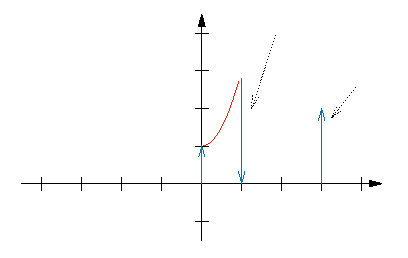
\includegraphics[width={180.00bp},height={108.00bp}]{figura_03_18}}%
    \gplfronttext
  \end{picture}%
\endgroup

    \end{minipage}
    \begin{minipage}{.4\textwidth}
        \centering
        % GNUPLOT: LaTeX picture with Postscript
\begingroup
  \makeatletter
  \providecommand\color[2][]{%
    \GenericError{(gnuplot) \space\space\space\@spaces}{%
      Package color not loaded in conjunction with
      terminal option `colourtext'%
    }{See the gnuplot documentation for explanation.%
    }{Either use 'blacktext' in gnuplot or load the package
      color.sty in LaTeX.}%
    \renewcommand\color[2][]{}%
  }%
  \providecommand\includegraphics[2][]{%
    \GenericError{(gnuplot) \space\space\space\@spaces}{%
      Package graphicx or graphics not loaded%
    }{See the gnuplot documentation for explanation.%
    }{The gnuplot epslatex terminal needs graphicx.sty or graphics.sty.}%
    \renewcommand\includegraphics[2][]{}%
  }%
  \providecommand\rotatebox[2]{#2}%
  \@ifundefined{ifGPcolor}{%
    \newif\ifGPcolor
    \GPcolorfalse
  }{}%
  \@ifundefined{ifGPblacktext}{%
    \newif\ifGPblacktext
    \GPblacktexttrue
  }{}%
  % define a \g@addto@macro without @ in the name:
  \let\gplgaddtomacro\g@addto@macro
  % define empty templates for all commands taking text:
  \gdef\gplbacktext{}%
  \gdef\gplfronttext{}%
  \makeatother
  \ifGPblacktext
    % no textcolor at all
    \def\colorrgb#1{}%
    \def\colorgray#1{}%
  \else
    % gray or color?
    \ifGPcolor
      \def\colorrgb#1{\color[rgb]{#1}}%
      \def\colorgray#1{\color[gray]{#1}}%
      \expandafter\def\csname LTw\endcsname{\color{white}}%
      \expandafter\def\csname LTb\endcsname{\color{black}}%
      \expandafter\def\csname LTa\endcsname{\color{black}}%
      \expandafter\def\csname LT0\endcsname{\color[rgb]{1,0,0}}%
      \expandafter\def\csname LT1\endcsname{\color[rgb]{0,1,0}}%
      \expandafter\def\csname LT2\endcsname{\color[rgb]{0,0,1}}%
      \expandafter\def\csname LT3\endcsname{\color[rgb]{1,0,1}}%
      \expandafter\def\csname LT4\endcsname{\color[rgb]{0,1,1}}%
      \expandafter\def\csname LT5\endcsname{\color[rgb]{1,1,0}}%
      \expandafter\def\csname LT6\endcsname{\color[rgb]{0,0,0}}%
      \expandafter\def\csname LT7\endcsname{\color[rgb]{1,0.3,0}}%
      \expandafter\def\csname LT8\endcsname{\color[rgb]{0.5,0.5,0.5}}%
    \else
      % gray
      \def\colorrgb#1{\color{black}}%
      \def\colorgray#1{\color[gray]{#1}}%
      \expandafter\def\csname LTw\endcsname{\color{white}}%
      \expandafter\def\csname LTb\endcsname{\color{black}}%
      \expandafter\def\csname LTa\endcsname{\color{black}}%
      \expandafter\def\csname LT0\endcsname{\color{black}}%
      \expandafter\def\csname LT1\endcsname{\color{black}}%
      \expandafter\def\csname LT2\endcsname{\color{black}}%
      \expandafter\def\csname LT3\endcsname{\color{black}}%
      \expandafter\def\csname LT4\endcsname{\color{black}}%
      \expandafter\def\csname LT5\endcsname{\color{black}}%
      \expandafter\def\csname LT6\endcsname{\color{black}}%
      \expandafter\def\csname LT7\endcsname{\color{black}}%
      \expandafter\def\csname LT8\endcsname{\color{black}}%
    \fi
  \fi
    \setlength{\unitlength}{0.0500bp}%
    \ifx\gptboxheight\undefined%
      \newlength{\gptboxheight}%
      \newlength{\gptboxwidth}%
      \newsavebox{\gptboxtext}%
    \fi%
    \setlength{\fboxrule}{0.5pt}%
    \setlength{\fboxsep}{1pt}%
    \definecolor{tbcol}{rgb}{1,1,1}%
\begin{picture}(3600.00,2160.00)%
    \gplgaddtomacro\gplbacktext{%
      \csname LTb\endcsname%%
      \put(1680,192){\makebox(0,0)[r]{\strut{}}}%
      \put(1680,553){\makebox(0,0)[r]{\strut{}}}%
      \put(1680,915){\makebox(0,0)[r]{\strut{}}}%
      \put(1680,1276){\makebox(0,0)[r]{\strut{}}}%
      \put(1680,1638){\makebox(0,0)[r]{\strut{}}}%
      \put(1680,1999){\makebox(0,0)[r]{\strut{}}}%
      \put(240,330){\makebox(0,0){\strut{}}}%
      \put(624,330){\makebox(0,0){\strut{}}}%
      \put(1008,330){\makebox(0,0){\strut{}}}%
      \put(1392,330){\makebox(0,0){\strut{}}}%
      \put(1776,330){\makebox(0,0){\strut{}}}%
      \put(2159,330){\makebox(0,0){\strut{}}}%
      \put(2543,330){\makebox(0,0){\strut{}}}%
      \put(2927,330){\makebox(0,0){\strut{}}}%
      \put(3311,330){\makebox(0,0){\strut{}}}%
      \csname LTb\endcsname%%
      \put(3580,553){\makebox(0,0)[l]{\strut{}$t$}}%
      \put(1219,2107){\makebox(0,0)[l]{\strut{}$f^\prime(t)$}}%
      \put(2121,337){\makebox(0,0)[l]{\strut{}$t_1$}}%
      \put(2889,337){\makebox(0,0)[l]{\strut{}$t_2$}}%
      \put(1871,734){\makebox(0,0)[l]{\strut{}$k_0\delta(t)$}}%
      \put(2255,11){\makebox(0,0)[l]{\strut{}$-k_1\delta(t-t_1)$}}%
      \put(3023,1005){\makebox(0,0)[l]{\strut{}$k_2\delta(t-t_2)$}}%
    }%
    \gplgaddtomacro\gplfronttext{%
    }%
    \gplbacktext
    \put(0,0){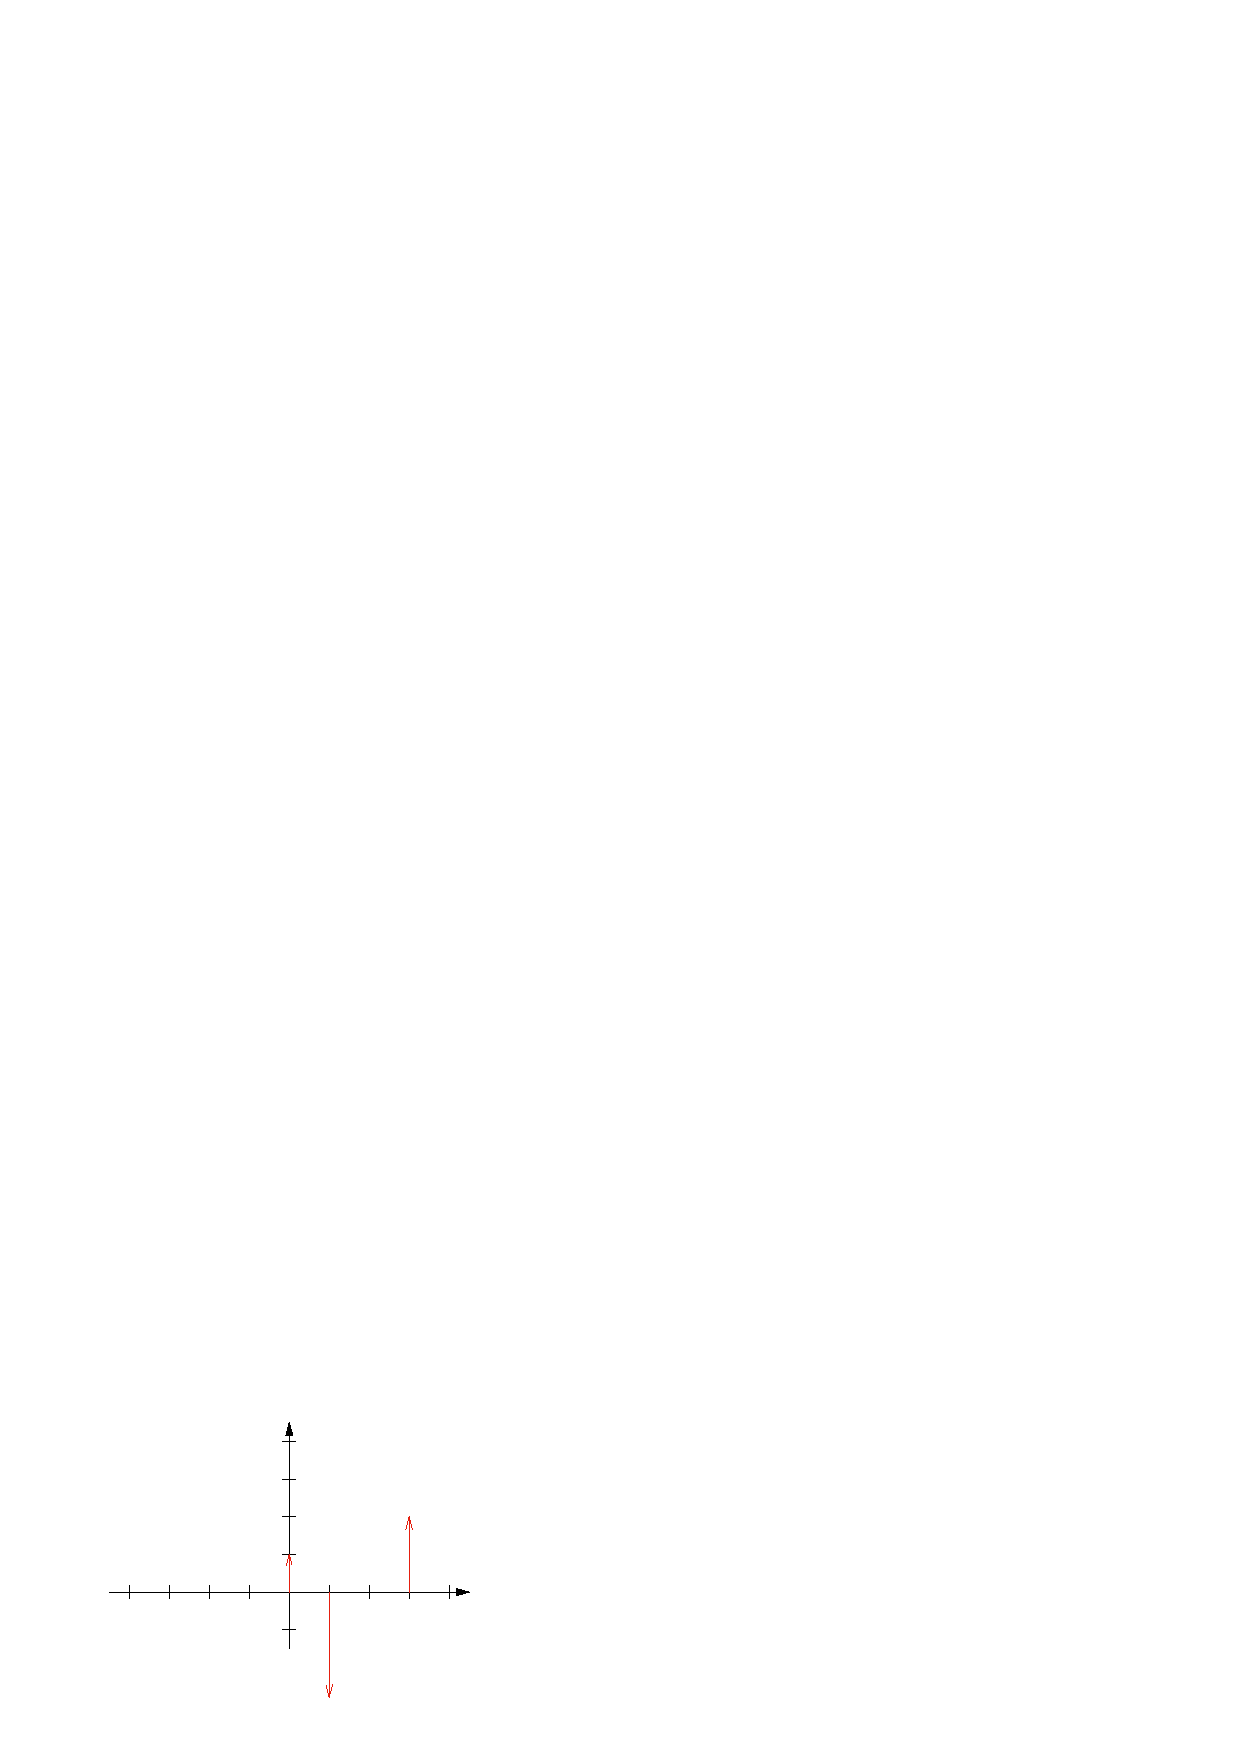
\includegraphics[width={180.00bp},height={108.00bp}]{figura_03_19}}%
    \gplfronttext
  \end{picture}%
\endgroup

    \end{minipage}
\end{figure}

\section{Series de \emph{Fourier} por el método de diferenciación}
\begin{minipage}{.5\linewidth}
    \begin{equation*}
        f(t)=\sum_{n=-\infty}^{\infty}c_n\,e^{jn\omega_0\,t}
    \end{equation*}
\end{minipage}
\begin{minipage}{.5\linewidth}
    \begin{equation*}
        c_n=\frac{1}{T}\int_0^T\,f(t)\,e^{-jn\omega_0\,t}\,dt
    \end{equation*}
\end{minipage}
\begin{minipage}{.5\linewidth}
    \begin{equation*}
        f^\prime(t)=\sum_{n=-\infty}^{\infty}jn\omega_0\,c_n\,e^{jn\omega_0\,t}
    \end{equation*}
\end{minipage}
\begin{minipage}{.5\linewidth}
    \begin{equation}
        \gamma^\prime_n=\frac{1}{T}\int_0^T\,f^\prime(t)\,e^{-jn\omega_0\,t}\,dt
    \end{equation}
\end{minipage}
\begin{minipage}{.5\linewidth}
    \begin{equation*}
        f^{\prime\prime}(t)
            =\sum_{n=-\infty}^{\infty}{(jn\omega_0)}^2\,c_n\,e^{jn\omega_0\,t}
    \end{equation*}
\end{minipage}
\begin{minipage}{.5\linewidth}
    \begin{equation}
        \gamma^{\prime\prime}_n
            =\frac{1}{T}\int_0^T\,f^{\prime\prime}(t)\,e^{-jn\omega_0\,t}\,dt
    \end{equation}
\end{minipage}
\begin{minipage}{.5\linewidth}
    \begin{equation*}
        f^{(k)}(t)
            =\sum_{n=-\infty}^{\infty}{(jn\omega_0)}^k\,c_n\,e^{jn\omega_0\,t}
    \end{equation*}
\end{minipage}
\begin{minipage}{.5\linewidth}
    \begin{equation}
        \gamma^{(k)}_n
            =\frac{1}{T}\int_0^T\,f^{(k)}(t)\,e^{-jn\omega_0\,t}\,dt
    \end{equation}
\end{minipage}

\begin{itemize}
    \item Se deriva $f(t)$ hasta anularla y calcular para cada derivada:
    $\gamma^{(k)}_n$
    \item Las derivadas de $f(t)$ solo van a tomar en cuenta los impulsos
    obtenidos de los saltos previos.
    \item El coeficiente complejo $c_n$ se obtendrá de la forma:
    \begin{equation}
        c_n=c^\prime_n+c^{\prime\prime}_n+\cdots+c^{(k)}_n
    \end{equation}
    Donde:
    \begin{equation}
        c^\prime_n=\frac{\gamma^\prime_n}{jn\omega_0}
    \end{equation}
    \begin{equation}
        c^{\prime\prime}_n=\frac{\gamma^{\prime\prime}_n}{{(jn\omega_0)}^2}
    \end{equation}
    \begin{equation}
        c^{(k)}_n=\frac{\gamma^{(k)}_n}{{(jn\omega_0)}^k}
    \end{equation}
\end{itemize}

\section{Espectros de frecuencia discreta}
Los espectros de frecuencia serán gráficas discretas de modulo y argumento del
coeficiente complejo de \emph{Fourier} en función de múltiplos de la frecuencia:
$\omega_0$.
\begin{equation*}
    f(t)=\sum_{n=-\infty}^\infty\,c_n\,e^{jn\omega_0\,t}
\end{equation*}
\begin{equation*}
    c_n=A_n+jB_n
\end{equation*}
\begin{equation*}
\left.\begin{aligned}
    |c_n|&=\sqrt{A_n^2+B_n^2}\\
    \theta_n&=\arctan\left(\frac{B_n}{A_n}\right)\\
\end{aligned}\right\}
\text{funciones discretas de }n\omega_0\quad\,n\in\mathbb{Z}
\end{equation*}
\begin{figure}[H]
    \centering
    \begin{minipage}{.4\textwidth}
        \centering
        % GNUPLOT: LaTeX picture with Postscript
\begingroup
  \makeatletter
  \providecommand\color[2][]{%
    \GenericError{(gnuplot) \space\space\space\@spaces}{%
      Package color not loaded in conjunction with
      terminal option `colourtext'%
    }{See the gnuplot documentation for explanation.%
    }{Either use 'blacktext' in gnuplot or load the package
      color.sty in LaTeX.}%
    \renewcommand\color[2][]{}%
  }%
  \providecommand\includegraphics[2][]{%
    \GenericError{(gnuplot) \space\space\space\@spaces}{%
      Package graphicx or graphics not loaded%
    }{See the gnuplot documentation for explanation.%
    }{The gnuplot epslatex terminal needs graphicx.sty or graphics.sty.}%
    \renewcommand\includegraphics[2][]{}%
  }%
  \providecommand\rotatebox[2]{#2}%
  \@ifundefined{ifGPcolor}{%
    \newif\ifGPcolor
    \GPcolorfalse
  }{}%
  \@ifundefined{ifGPblacktext}{%
    \newif\ifGPblacktext
    \GPblacktexttrue
  }{}%
  % define a \g@addto@macro without @ in the name:
  \let\gplgaddtomacro\g@addto@macro
  % define empty templates for all commands taking text:
  \gdef\gplbacktext{}%
  \gdef\gplfronttext{}%
  \makeatother
  \ifGPblacktext
    % no textcolor at all
    \def\colorrgb#1{}%
    \def\colorgray#1{}%
  \else
    % gray or color?
    \ifGPcolor
      \def\colorrgb#1{\color[rgb]{#1}}%
      \def\colorgray#1{\color[gray]{#1}}%
      \expandafter\def\csname LTw\endcsname{\color{white}}%
      \expandafter\def\csname LTb\endcsname{\color{black}}%
      \expandafter\def\csname LTa\endcsname{\color{black}}%
      \expandafter\def\csname LT0\endcsname{\color[rgb]{1,0,0}}%
      \expandafter\def\csname LT1\endcsname{\color[rgb]{0,1,0}}%
      \expandafter\def\csname LT2\endcsname{\color[rgb]{0,0,1}}%
      \expandafter\def\csname LT3\endcsname{\color[rgb]{1,0,1}}%
      \expandafter\def\csname LT4\endcsname{\color[rgb]{0,1,1}}%
      \expandafter\def\csname LT5\endcsname{\color[rgb]{1,1,0}}%
      \expandafter\def\csname LT6\endcsname{\color[rgb]{0,0,0}}%
      \expandafter\def\csname LT7\endcsname{\color[rgb]{1,0.3,0}}%
      \expandafter\def\csname LT8\endcsname{\color[rgb]{0.5,0.5,0.5}}%
    \else
      % gray
      \def\colorrgb#1{\color{black}}%
      \def\colorgray#1{\color[gray]{#1}}%
      \expandafter\def\csname LTw\endcsname{\color{white}}%
      \expandafter\def\csname LTb\endcsname{\color{black}}%
      \expandafter\def\csname LTa\endcsname{\color{black}}%
      \expandafter\def\csname LT0\endcsname{\color{black}}%
      \expandafter\def\csname LT1\endcsname{\color{black}}%
      \expandafter\def\csname LT2\endcsname{\color{black}}%
      \expandafter\def\csname LT3\endcsname{\color{black}}%
      \expandafter\def\csname LT4\endcsname{\color{black}}%
      \expandafter\def\csname LT5\endcsname{\color{black}}%
      \expandafter\def\csname LT6\endcsname{\color{black}}%
      \expandafter\def\csname LT7\endcsname{\color{black}}%
      \expandafter\def\csname LT8\endcsname{\color{black}}%
    \fi
  \fi
    \setlength{\unitlength}{0.0500bp}%
    \ifx\gptboxheight\undefined%
      \newlength{\gptboxheight}%
      \newlength{\gptboxwidth}%
      \newsavebox{\gptboxtext}%
    \fi%
    \setlength{\fboxrule}{0.5pt}%
    \setlength{\fboxsep}{1pt}%
    \definecolor{tbcol}{rgb}{1,1,1}%
\begin{picture}(3168.00,2160.00)%
    \gplgaddtomacro\gplbacktext{%
      \csname LTb\endcsname%%
      \put(1464,192){\makebox(0,0)[r]{\strut{}}}%
      \put(1464,553){\makebox(0,0)[r]{\strut{}}}%
      \put(1464,915){\makebox(0,0)[r]{\strut{}}}%
      \put(1464,1276){\makebox(0,0)[r]{\strut{}}}%
      \put(1464,1638){\makebox(0,0)[r]{\strut{}}}%
      \put(1464,1999){\makebox(0,0)[r]{\strut{}}}%
      \put(240,330){\makebox(0,0){\strut{}}}%
      \put(570,330){\makebox(0,0){\strut{}}}%
      \put(900,330){\makebox(0,0){\strut{}}}%
      \put(1230,330){\makebox(0,0){\strut{}}}%
      \put(1560,330){\makebox(0,0){\strut{}}}%
      \put(1889,330){\makebox(0,0){\strut{}}}%
      \put(2219,330){\makebox(0,0){\strut{}}}%
      \put(2549,330){\makebox(0,0){\strut{}}}%
      \put(2879,330){\makebox(0,0){\strut{}}}%
      \csname LTb\endcsname%%
      \put(3110,553){\makebox(0,0)[l]{\strut{}$n\omega_0$}}%
      \put(1081,2107){\makebox(0,0)[l]{\strut{}$|c_n|$}}%
      \put(273,337){\makebox(0,0)[l]{\strut{}$-3\omega_0$}}%
      \put(1032,337){\makebox(0,0)[l]{\strut{}$ -\omega_0$}}%
      \put(1856,337){\makebox(0,0)[l]{\strut{}$  \omega_0$}}%
      \put(2417,337){\makebox(0,0)[l]{\strut{}$ 3\omega_0$}}%
    }%
    \gplgaddtomacro\gplfronttext{%
    }%
    \gplbacktext
    \put(0,0){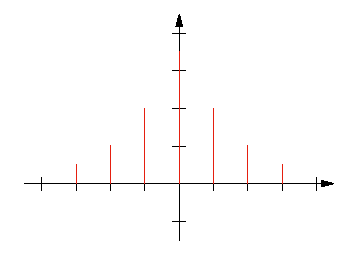
\includegraphics[width={158.40bp},height={108.00bp}]{figura_03_20}}%
    \gplfronttext
  \end{picture}%
\endgroup

        \captionsetup{labelformat=empty}
        \caption{Espectro de amplitud o módulo}
    \end{minipage}
    \begin{minipage}{.4\textwidth}
        \centering
        % GNUPLOT: LaTeX picture with Postscript
\begingroup
  \makeatletter
  \providecommand\color[2][]{%
    \GenericError{(gnuplot) \space\space\space\@spaces}{%
      Package color not loaded in conjunction with
      terminal option `colourtext'%
    }{See the gnuplot documentation for explanation.%
    }{Either use 'blacktext' in gnuplot or load the package
      color.sty in LaTeX.}%
    \renewcommand\color[2][]{}%
  }%
  \providecommand\includegraphics[2][]{%
    \GenericError{(gnuplot) \space\space\space\@spaces}{%
      Package graphicx or graphics not loaded%
    }{See the gnuplot documentation for explanation.%
    }{The gnuplot epslatex terminal needs graphicx.sty or graphics.sty.}%
    \renewcommand\includegraphics[2][]{}%
  }%
  \providecommand\rotatebox[2]{#2}%
  \@ifundefined{ifGPcolor}{%
    \newif\ifGPcolor
    \GPcolorfalse
  }{}%
  \@ifundefined{ifGPblacktext}{%
    \newif\ifGPblacktext
    \GPblacktexttrue
  }{}%
  % define a \g@addto@macro without @ in the name:
  \let\gplgaddtomacro\g@addto@macro
  % define empty templates for all commands taking text:
  \gdef\gplbacktext{}%
  \gdef\gplfronttext{}%
  \makeatother
  \ifGPblacktext
    % no textcolor at all
    \def\colorrgb#1{}%
    \def\colorgray#1{}%
  \else
    % gray or color?
    \ifGPcolor
      \def\colorrgb#1{\color[rgb]{#1}}%
      \def\colorgray#1{\color[gray]{#1}}%
      \expandafter\def\csname LTw\endcsname{\color{white}}%
      \expandafter\def\csname LTb\endcsname{\color{black}}%
      \expandafter\def\csname LTa\endcsname{\color{black}}%
      \expandafter\def\csname LT0\endcsname{\color[rgb]{1,0,0}}%
      \expandafter\def\csname LT1\endcsname{\color[rgb]{0,1,0}}%
      \expandafter\def\csname LT2\endcsname{\color[rgb]{0,0,1}}%
      \expandafter\def\csname LT3\endcsname{\color[rgb]{1,0,1}}%
      \expandafter\def\csname LT4\endcsname{\color[rgb]{0,1,1}}%
      \expandafter\def\csname LT5\endcsname{\color[rgb]{1,1,0}}%
      \expandafter\def\csname LT6\endcsname{\color[rgb]{0,0,0}}%
      \expandafter\def\csname LT7\endcsname{\color[rgb]{1,0.3,0}}%
      \expandafter\def\csname LT8\endcsname{\color[rgb]{0.5,0.5,0.5}}%
    \else
      % gray
      \def\colorrgb#1{\color{black}}%
      \def\colorgray#1{\color[gray]{#1}}%
      \expandafter\def\csname LTw\endcsname{\color{white}}%
      \expandafter\def\csname LTb\endcsname{\color{black}}%
      \expandafter\def\csname LTa\endcsname{\color{black}}%
      \expandafter\def\csname LT0\endcsname{\color{black}}%
      \expandafter\def\csname LT1\endcsname{\color{black}}%
      \expandafter\def\csname LT2\endcsname{\color{black}}%
      \expandafter\def\csname LT3\endcsname{\color{black}}%
      \expandafter\def\csname LT4\endcsname{\color{black}}%
      \expandafter\def\csname LT5\endcsname{\color{black}}%
      \expandafter\def\csname LT6\endcsname{\color{black}}%
      \expandafter\def\csname LT7\endcsname{\color{black}}%
      \expandafter\def\csname LT8\endcsname{\color{black}}%
    \fi
  \fi
    \setlength{\unitlength}{0.0500bp}%
    \ifx\gptboxheight\undefined%
      \newlength{\gptboxheight}%
      \newlength{\gptboxwidth}%
      \newsavebox{\gptboxtext}%
    \fi%
    \setlength{\fboxrule}{0.5pt}%
    \setlength{\fboxsep}{1pt}%
    \definecolor{tbcol}{rgb}{1,1,1}%
\begin{picture}(3168.00,2160.00)%
    \gplgaddtomacro\gplbacktext{%
      \csname LTb\endcsname%%
      \put(1464,192){\makebox(0,0)[r]{\strut{}}}%
      \put(1464,553){\makebox(0,0)[r]{\strut{}}}%
      \put(1464,915){\makebox(0,0)[r]{\strut{}}}%
      \put(1464,1276){\makebox(0,0)[r]{\strut{}}}%
      \put(1464,1638){\makebox(0,0)[r]{\strut{}}}%
      \put(1464,1999){\makebox(0,0)[r]{\strut{}}}%
      \put(240,330){\makebox(0,0){\strut{}}}%
      \put(570,330){\makebox(0,0){\strut{}}}%
      \put(900,330){\makebox(0,0){\strut{}}}%
      \put(1230,330){\makebox(0,0){\strut{}}}%
      \put(1560,330){\makebox(0,0){\strut{}}}%
      \put(1889,330){\makebox(0,0){\strut{}}}%
      \put(2219,330){\makebox(0,0){\strut{}}}%
      \put(2549,330){\makebox(0,0){\strut{}}}%
      \put(2879,330){\makebox(0,0){\strut{}}}%
      \csname LTb\endcsname%%
      \put(3110,553){\makebox(0,0)[l]{\strut{}$n\omega_0$}}%
      \put(1081,2107){\makebox(0,0)[l]{\strut{}$\theta_n$}}%
      \put(273,337){\makebox(0,0)[l]{\strut{}$-3\omega_0$}}%
      \put(1032,337){\makebox(0,0)[l]{\strut{}$ -\omega_0$}}%
      \put(1856,337){\makebox(0,0)[l]{\strut{}$  \omega_0$}}%
      \put(2417,337){\makebox(0,0)[l]{\strut{}$ 3\omega_0$}}%
    }%
    \gplgaddtomacro\gplfronttext{%
    }%
    \gplbacktext
    \put(0,0){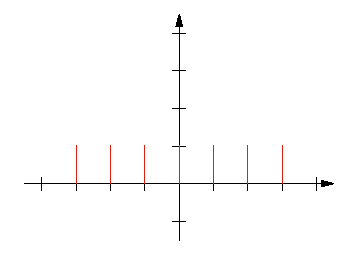
\includegraphics[width={158.40bp},height={108.00bp}]{figura_03_21}}%
    \gplfronttext
  \end{picture}%
\endgroup

        \captionsetup{labelformat=empty}
        \caption{Espectro de fase o argumento}
    \end{minipage}
\end{figure}

\section{Teorema de la multiplicación}
Dadas dos funciones periódicas con el mismo periodo $T$: $f_1(t)$ y $f_2(t)$.

Donde: $c_1n$ y $c_2n$, son los respectivos coeficientes complejos de
\emph{Fourier}.
\begin{equation}
    \frac{1}{T}\int_0^T\,f_1(t)f_2(t)\,dt
        =\sum_{n={-\infty}}^\infty\,c_1(n)\,c_2(-n)
        =\sum_{n={-\infty}}^\infty\,c_1(-n)\,c_2(n)
\end{equation}

\underline{Prueba}:

\begin{equation*}
\begin{split}
    \frac{1}{T}\int_0^T\,f_1(t)f_2(t)\,dt
        &=\frac{1}{T}\int_0^T\left[
            \sum_{n={-\infty}}^\infty\,c_1(n)\,e^{jn\omega_0\,t}
        \right]\,f_2(t)\,dt\\
        &=\sum_{n={-\infty}}^\infty\,c_1(n)\,\frac{1}{T}
            \int_0^T\,f_2(t)\,e^{jn\omega_0\,t}\,dt\\
        &=\sum_{n={-\infty}}^\infty\,c_1(n)c_2(-n)
\end{split}
\end{equation*}

\section{Teorema de \emph{Parseval}}
Sea: $f_1(t)=f_2(t)=f(t)$, con coeficientes de \emph{Fourier}:
$c_1(n)=c_2(n)=c_n$:

Partiendo del teorema de multiplicación:
\begin{equation*}
\begin{split}
    \frac{1}{T}\int_0^T\,f^2(t)\,dt
        &=\sum_{n={-\infty}}^\infty\,c_{(n)}\,c_{(-n)}\\
        &=\sum_{n={-\infty}}^\infty\,c_{(n)}\,c_{(n)}^*\\
        &=\sum_{n={-\infty}}^\infty\,{|c_n|}^2\\
        &=c_0^2+\sum_{\substack{n=-\infty\\n\neq0}}^\infty\,{|c_n|}^2\\
\end{split}
\end{equation*}
\begin{equation*}
    c_n=\frac{a_n-jb_n}{2}
\end{equation*}
\begin{equation*}
    {|c_n|}^2=\frac{a_n^2+b_n^2}{4}
\end{equation*}
\begin{equation*}
\begin{split}
    \frac{1}{T}\int_0^T\,f^2(t)\,dt
        &=c_0^2+\sum_{\substack{n=-\infty\\n\neq0}}^\infty
            \frac{a_n^2+b_n^2}{4}\\
        &=c_0^2+\frac{1}{4}\sum_{n=1}^\infty(a_n^2+b_n^2)
            +\frac{1}{4}\sum_{n=-1}^{-\infty}(a_n^2+b_n^2)\\
\end{split}
\end{equation*}

Cambiando $n$ por $-n$:
\begin{equation*}
\begin{split}
    \frac{1}{T}\int_0^T\,f^2(t)\,dt
        &=c_0^2+\frac{1}{4}\sum_{n=1}^\infty(a_n^2+b_n^2)
            +\frac{1}{4}\sum_{-n=-1}^{-\infty}(a_{(-n)}^2+b_{(-n)}^2)\\
\end{split}
\end{equation*}

Sabiendo que:
\begin{equation*}
    a_n^2=a_{(-n)}^2
\end{equation*}
\begin{equation*}
    {(-b_n)}^2=b_n^2
\end{equation*}
\begin{equation*}
\begin{split}
    \frac{1}{T}\int_0^T\,f^2(t)\,dt
        &=c_0^2+\frac{1}{4}\sum_{n=1}^\infty(a_n^2+b_n^2)
            +\frac{1}{4}\sum_{n=1}^\infty(a_n^2+b_n^2)\\
        &=c_0^2+\frac{1}{2}\sum_{n=1}^\infty(a_n^2+b_n^2)
\end{split}
\end{equation*}

\begin{equation}
    \frac{1}{T}\int_0^T\,f^2(t)\,dt
        =c_0^2+\frac{1}{2}\sum_{n=1}^\infty(a_n^2+b_n^2)
\end{equation}

